\documentclass{beamer}
\usetheme{Madrid}
\usepackage{tikz}
\usetikzlibrary{fit,calc}
\usepackage{graphicx}
\usepackage{media9}
\usepackage{appendixnumberbeamer} % Excludes appendix frames from total frame count

\setbeamerfont{section in head/foot}{size=\small}
\setbeamerfont{footnote}{size=\tiny}

% Counter for the total number of slides in the section (set manually)
\newcounter{sectionframes}
\newcommand{\setsectionframes}[1]{%
  \setcounter{sectionframes}{#1}%
}

% New counter for the current frame number within a section
\newcounter{sectionframecount}
% Reset the local frame counter at the beginning of each section.
\AtBeginSection{\setcounter{sectionframecount}{0}}

% A command to draw progress dots given the current frame number in the section and the total frames.
\newcommand{\sectionprogress}[2]{%
  \tikzset{dot/.style={circle, draw, fill=black, inner sep=1.3pt}}%
  \tikzset{activedot/.style={circle, draw, fill=red, inner sep=1.3pt}}%
  \foreach \i in {1,...,#2}{%
    \ifnum\i>#1
      \tikz[baseline=-0.7ex]\node[dot] at (0,0) {};%
    \else
      \tikz[baseline=-0.7ex]\node[activedot] at (0,0) {};%
    \fi
    \hspace{1ex}%
  }%
}

% Custom headline: left side shows the current section name; right side shows the slide progress for the current section.
\setbeamertemplate{headline}{%
\begin{beamercolorbox}[wd=\paperwidth,ht=4ex,dp=1ex]{section in head/foot}
  \hbox{%
  \hspace*{1em}%
  \usebeamerfont{section in head/foot}\insertsectionhead%
  \hfill%
  \hspace{1em}%
  \sectionprogress{\value{sectionframecount}}{\value{sectionframes}}%
  }%
\end{beamercolorbox}%
}

\setbeamertemplate{footline}{%
  \leavevmode%
  \hbox{%
    \begin{beamercolorbox}[wd=.33\paperwidth,ht=2.5ex,dp=1ex,left]{author in head/foot}%
      \usebeamerfont{author in head/foot}\insertshortauthor%
    \end{beamercolorbox}%
    \begin{beamercolorbox}[wd=.34\paperwidth,ht=2.5ex,dp=1ex,center]{title in head/foot}%
      \usebeamerfont{title in head/foot}\insertshorttitle%
    \end{beamercolorbox}%
    \begin{beamercolorbox}[wd=.33\paperwidth,ht=2.5ex,dp=1ex,right]{date in head/foot}%
      \usebeamerfont{date in head/foot}\insertframenumber{} / \inserttotalframenumber\hspace*{2ex}%
    \end{beamercolorbox}%
  }%
  \vskip0pt%
}

\usecolortheme{beaver}

\title[CSE Community Seminar]{A Space-time Adaptive, Higher-order Finite Element Method for Sonic Boom}
\author[R. Trono Figueras]{%
  R. Trono Figueras\\[1ex]
  {\small David L. Darmofal, Marshall C. Galbraith, Steven R. Allmaras}
}
\institute{%
  MIT, Department of Aeronautics and Astronautics\\[1ex]
  {\scriptsize Funded by NASA (\#80NSSC22K0193)}
}
\date{April 11, 2025}

\begin{document}

%=============================================================================%
%=============================================================================%
%=============================================================================%
% Title page

\begin{frame}[plain]{CSE Community Seminar}
    \vspace{1.5cm}
    \titlepage
    \begin{tikzpicture}[remember picture,overlay]
      \node[anchor=north east, xshift=-11cm, yshift=-1cm]
        at (current page.north east) {
\includegraphics[height=1cm]{../figs/title_page/mit_logo.png}};
    \end{tikzpicture}

    \begin{tikzpicture}[remember picture,overlay]
      \node[anchor=north east, xshift=-1.5cm, yshift=-1cm]
        at (current page.north east) {
\includegraphics[height=1cm]{../figs/title_page/aeroastro_logo.jpg}};
    \end{tikzpicture}

    \begin{tikzpicture}[remember picture,overlay]
      \node[anchor=north east, xshift=-0.2cm, yshift=-1cm]
        at (current page.north east) {
\includegraphics[height=1cm]{../figs/title_page/mitccse_logo.jpeg}};
    \end{tikzpicture}
\end{frame}

%=============================================================================%
%=============================================================================%
%=============================================================================%
% Section: Motivation

\section{Motivation}

\setsectionframes{4}

%---------------------------------------------------------------%

\stepcounter{sectionframecount}
\begin{frame}[t]{Motivation For Sonic Boom Study}
  \vspace{-5pt}
  \begin{minipage}[t]{0.55\linewidth}
    \textbf{Ultimate goal:}

    Enable supersonic commercial flights overland.

    \uncover<2->
    {
    \vspace{10pt}
    \textbf{Main challenge:}

    \begin{itemize}
      \item Negative impact of sonic boom loudness on humans, other animals, and structures.
    \end{itemize}
    }

    \uncover<3->
    {
    \vspace{10pt}
    \textbf{Study sonic boom to:}
    \begin{itemize}
      \item Predict loudness sensitivities to airplane geometry.
      \item Perform airplane shape optimization to reduce loudness at ground.
    \end{itemize}
    }
  \end{minipage}

  \begin{tikzpicture}[remember picture,overlay]
    \node[anchor=north east, xshift=-0.2cm, yshift=-1.5cm]
      at (current page.north east) {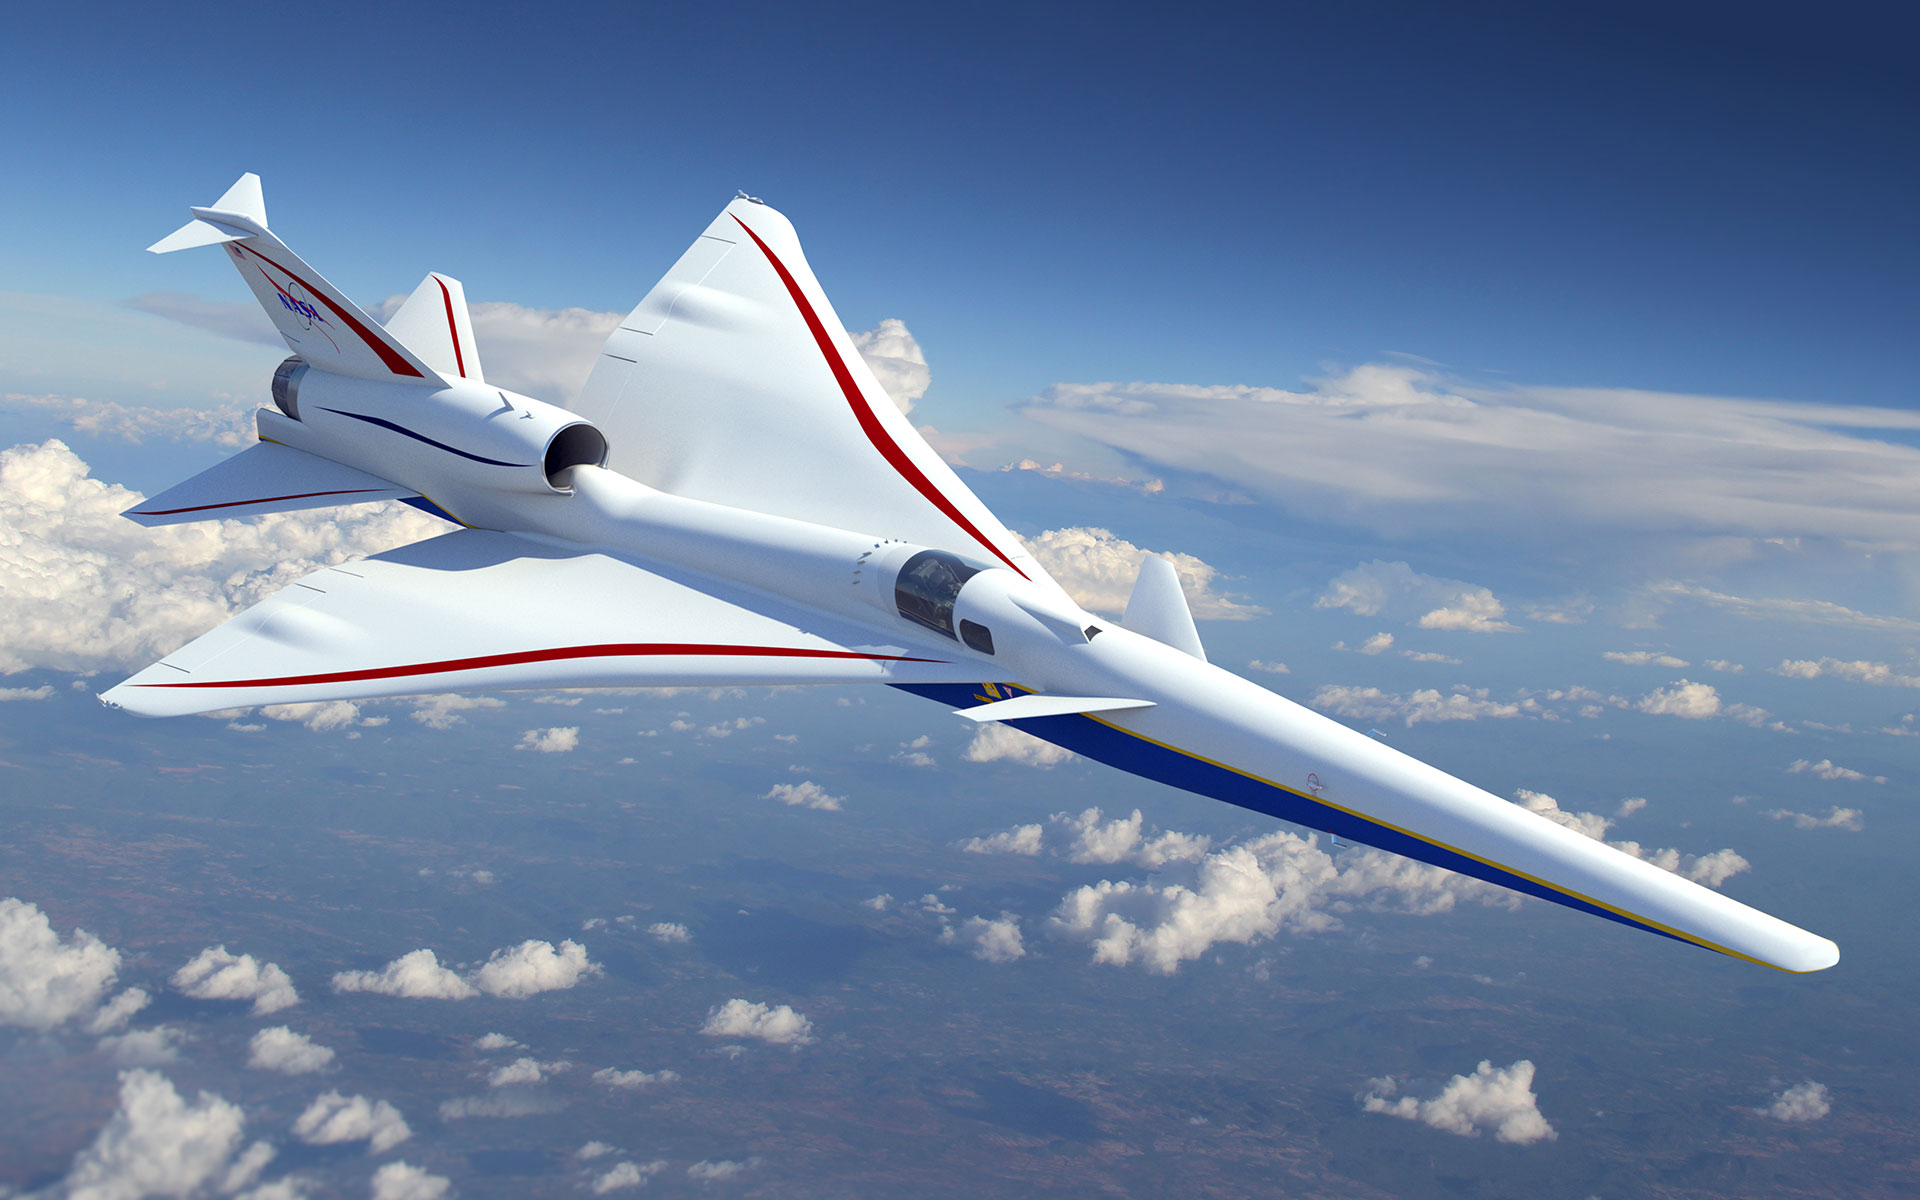
\includegraphics[height=3cm]{../figs/motivation/x59.jpg}};
    \node[anchor=north east, xshift=-2.3cm, yshift=-4.6cm]
      at (current page.north east) {\tiny\color{gray} Source: lockheedmartin.com};
    % https://www.lockheedmartin.com/en-us/products/x-59-quiet-supersonic.html
  \end{tikzpicture}

  \uncover<2->
  {
  \begin{tikzpicture}[remember picture,overlay]
    \node[anchor=north east, xshift=-0.2cm, yshift=-5.2cm]
      at (current page.north east) {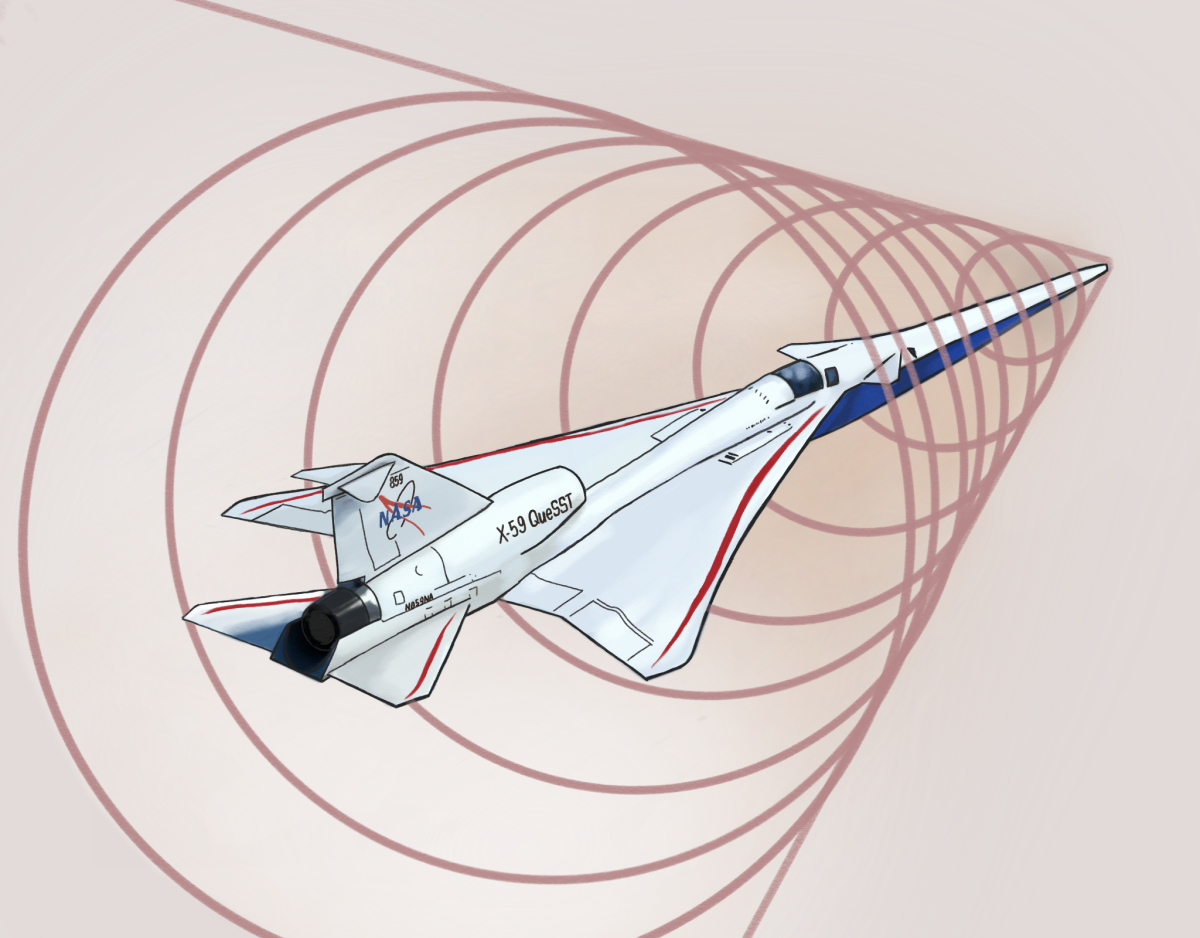
\includegraphics[height=3cm]{../figs/motivation/sonicboomX59Art.png}};
    \node[anchor=north east, xshift=-1.5cm, yshift=-8.3cm]
      at (current page.north east) {\tiny\color{gray} Source: michigandaily.com};
    % https://www.michigandaily.com/opinion/columns/bring-back-the-supersonic-jet-faster/
  \end{tikzpicture}
  }
\end{frame}

%---------------------------------------------------------------%

\stepcounter{sectionframecount}
\begin{frame}[t]{Solution Approach: Broad Picture}
  \begin{minipage}[t]{0.55\linewidth}
    \vspace{-20pt}
    Multidisciplinary design optimization\footnotemark:
    \begin{itemize}
      \uncover<2->
      {
      \item Parametric geometry generator.
      }
      \uncover<3->
      {
      \item CFD solver.
      \begin{itemize}
        \item Euler/Navier-Stokes in 3D.
        \item Uniform atmosphere.
      \end{itemize}
      }
      \uncover<4->
      {
      \tikz [remember picture,baseline] \node (start) {};
      \item \textit{Sonic boom propagation tool}
      \begin{itemize}
        \item 2D problem (or unsteady 1D).
        \item Weakly non-linear.
        \item Species relaxation.
        \item Non-uniform atmosphere. \tikz [remember picture,baseline] \node (end) {};
      \end{itemize}
      }
      \uncover<5->
      {
      \vspace{3pt}
      \item Numerical optimizer.
      }
    \end{itemize}
  \end{minipage}

  \uncover<6->
  {
  \begin{minipage}[t]{1\linewidth}
    \vspace{5pt}
    \tikz [remember picture,baseline] \node (start2) {}; Compute noise at ground \tikz [remember picture,baseline] \node (end2) {}; and
    \tikz [remember picture,baseline] \node (start3) {}; $\dfrac{d(\text{Noise})}{dX} = \dfrac{d (\text{Noise})}{d p_{nf}} \dfrac{d p_{nf}}{d X}$ \tikz [remember picture,baseline] \node (end3) {};.
  \end{minipage}
  }

  \uncover<4->
  {
  \begin{tikzpicture}[remember picture,overlay]
    \node[draw=red, dashed, thick, inner xsep=15pt, inner ysep=2pt,
          fit=(start) (end), xshift=-0.7mm, yshift=-0.4mm] {};
  \end{tikzpicture}
  }

  \begin{tikzpicture}[remember picture,overlay]
    \uncover<2->
    {
    \node (img) [anchor=north east, xshift=-0.2cm, yshift=-1.5cm, opacity=0.1]
      at (current page.north east) {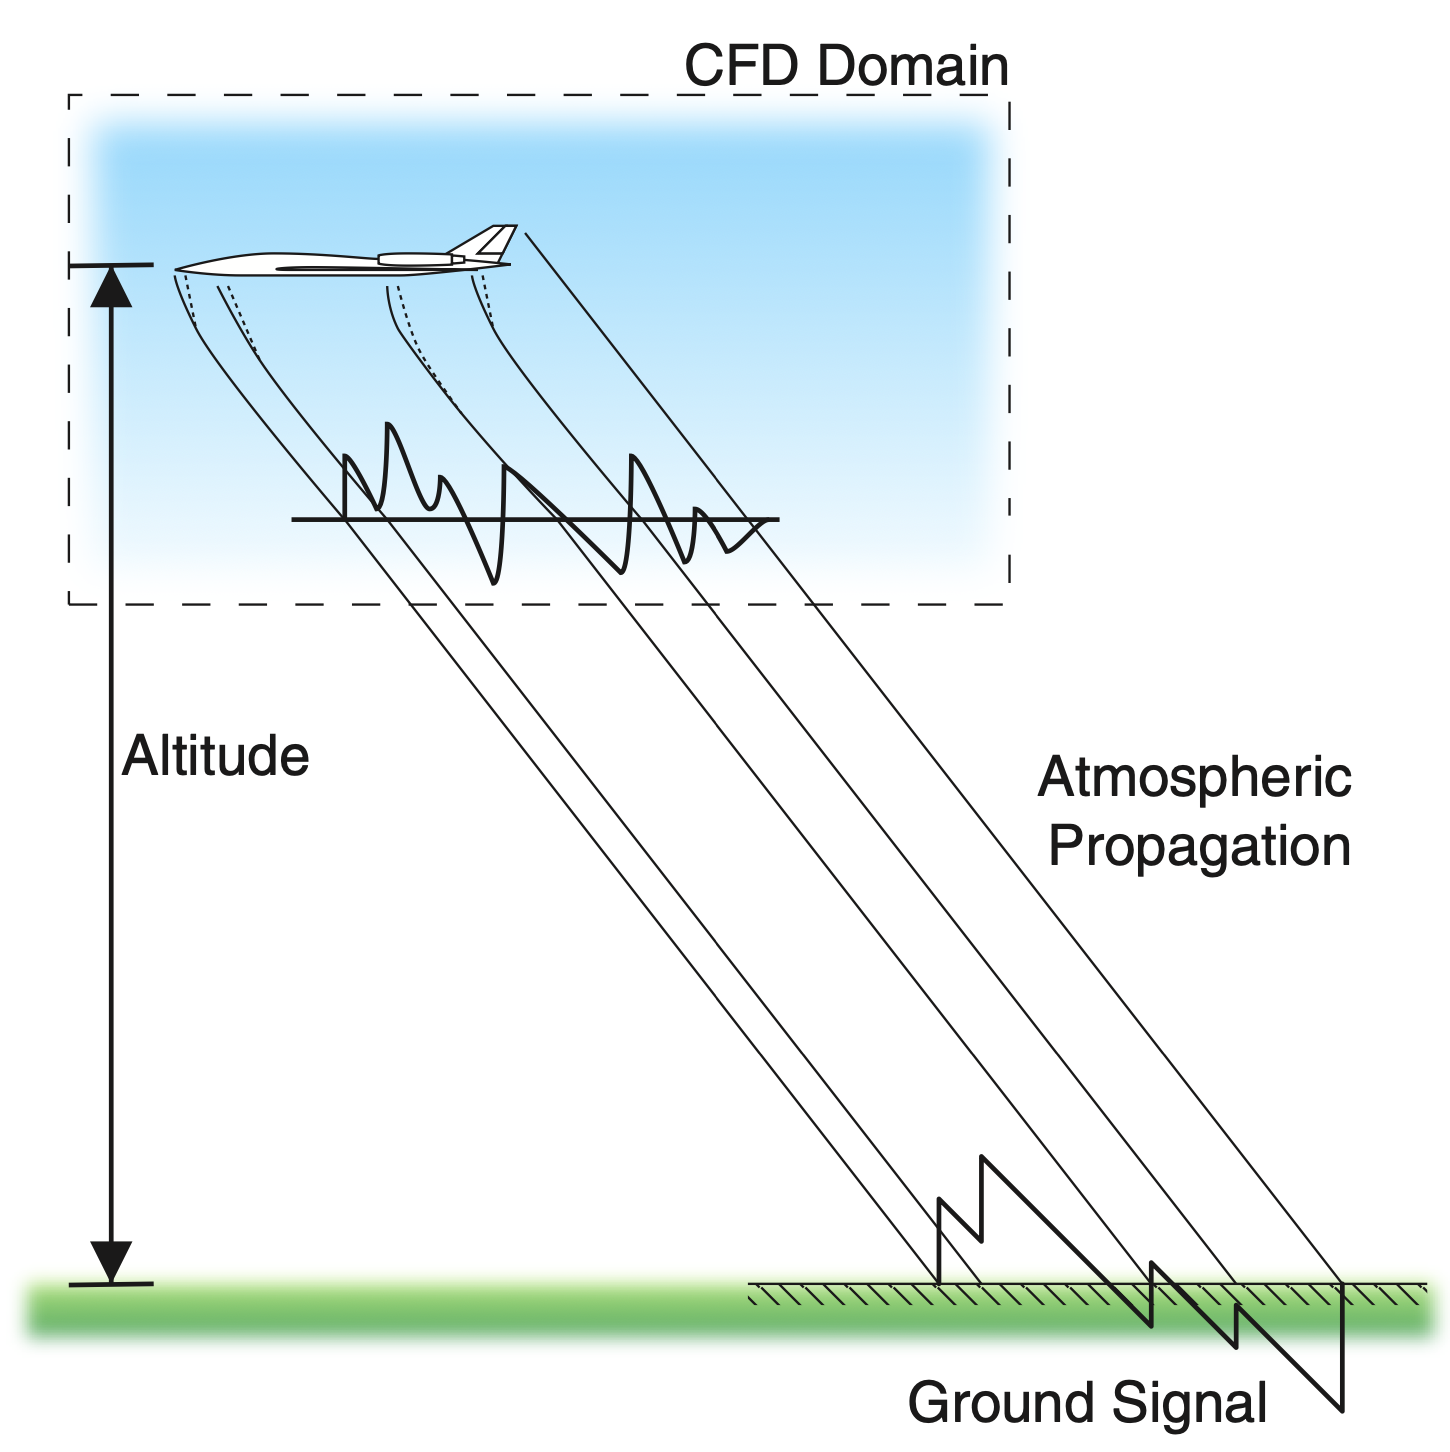
\includegraphics[height=5.5cm]{../figs/motivation/CFDandProp.png}};
    }



    \uncover<2->
    {
      \node[anchor=north east, xshift=-4.4cm, yshift=-6.8cm]
      at (current page.north east) {\tiny\color{gray} Source: [1]};
      }

      \uncover<2->
      {
        % Define coordinates for the region to emphasize relative to the image node.
        % These coordinates are offsets from the image's north west corner.
        \coordinate (clipA) at ($(img.north west)+(0.7cm,-0.6cm)$);
        \coordinate (clipB) at ($(img.north west)+(2.2cm,-1.3cm)$);
        % Overlay a copy of the image clipped to the region of interest (full opacity).
        \begin{scope}[remember picture,overlay]
          \clip (clipA) rectangle (clipB);
          \node [anchor=north east, xshift=-0.2cm, yshift=-1.5cm]
          at (current page.north east) {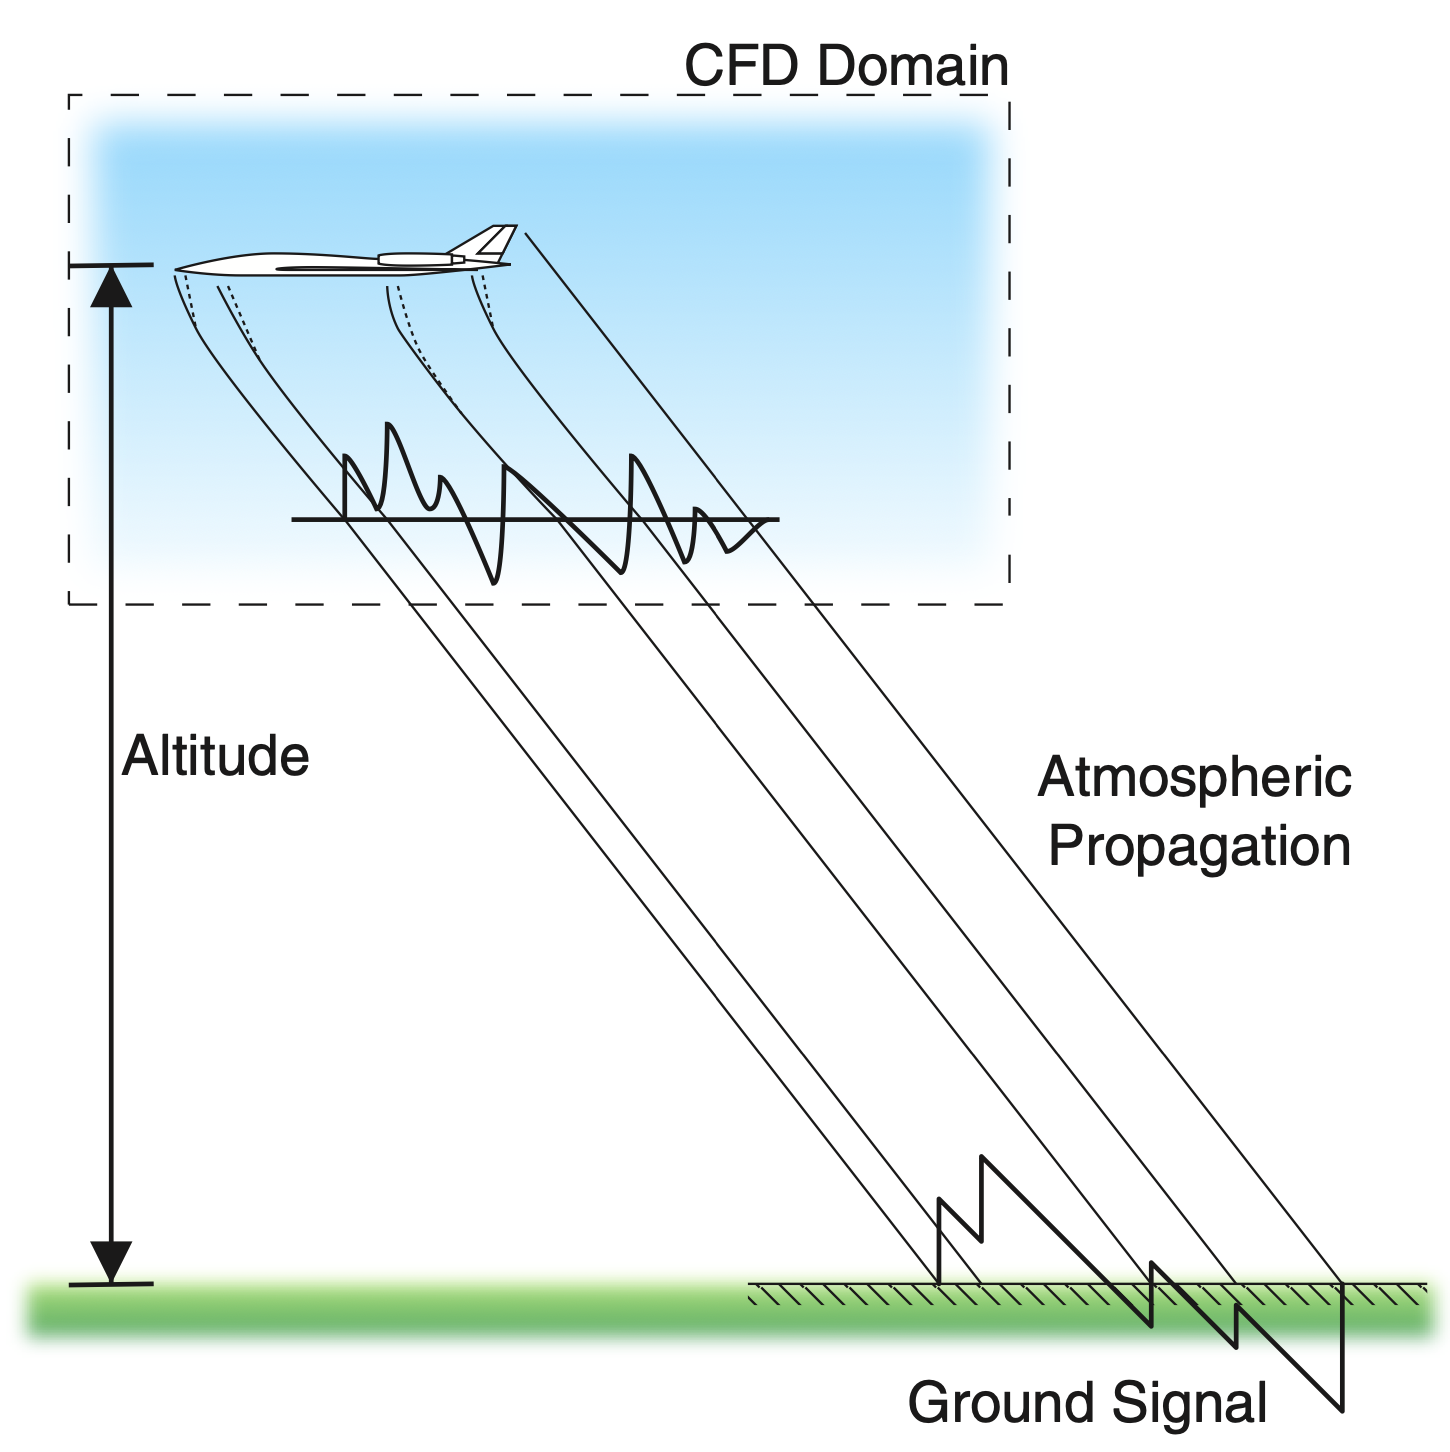
\includegraphics[height=5.5cm]{../figs/motivation/CFDandProp.png}};
        \end{scope}
        }



  \uncover<3->
  {
  % Define coordinates for the region to emphasize relative to the image node.
    % These coordinates are offsets from the image's north west corner.
      \coordinate (clipAA) at ($(img.north west)+(0.4cm,-0.3cm)$);
      \coordinate (clipBB) at ($(img.north west)+(5.2cm,-2.45cm)$);
      % Overlay a copy of the image clipped to the region of interest (full opacity).
      \begin{scope}[remember picture,overlay]
        \clip (clipAA) rectangle (clipBB);
        \node [anchor=north east, xshift=-0.2cm, yshift=-1.5cm]
        at (current page.north east) {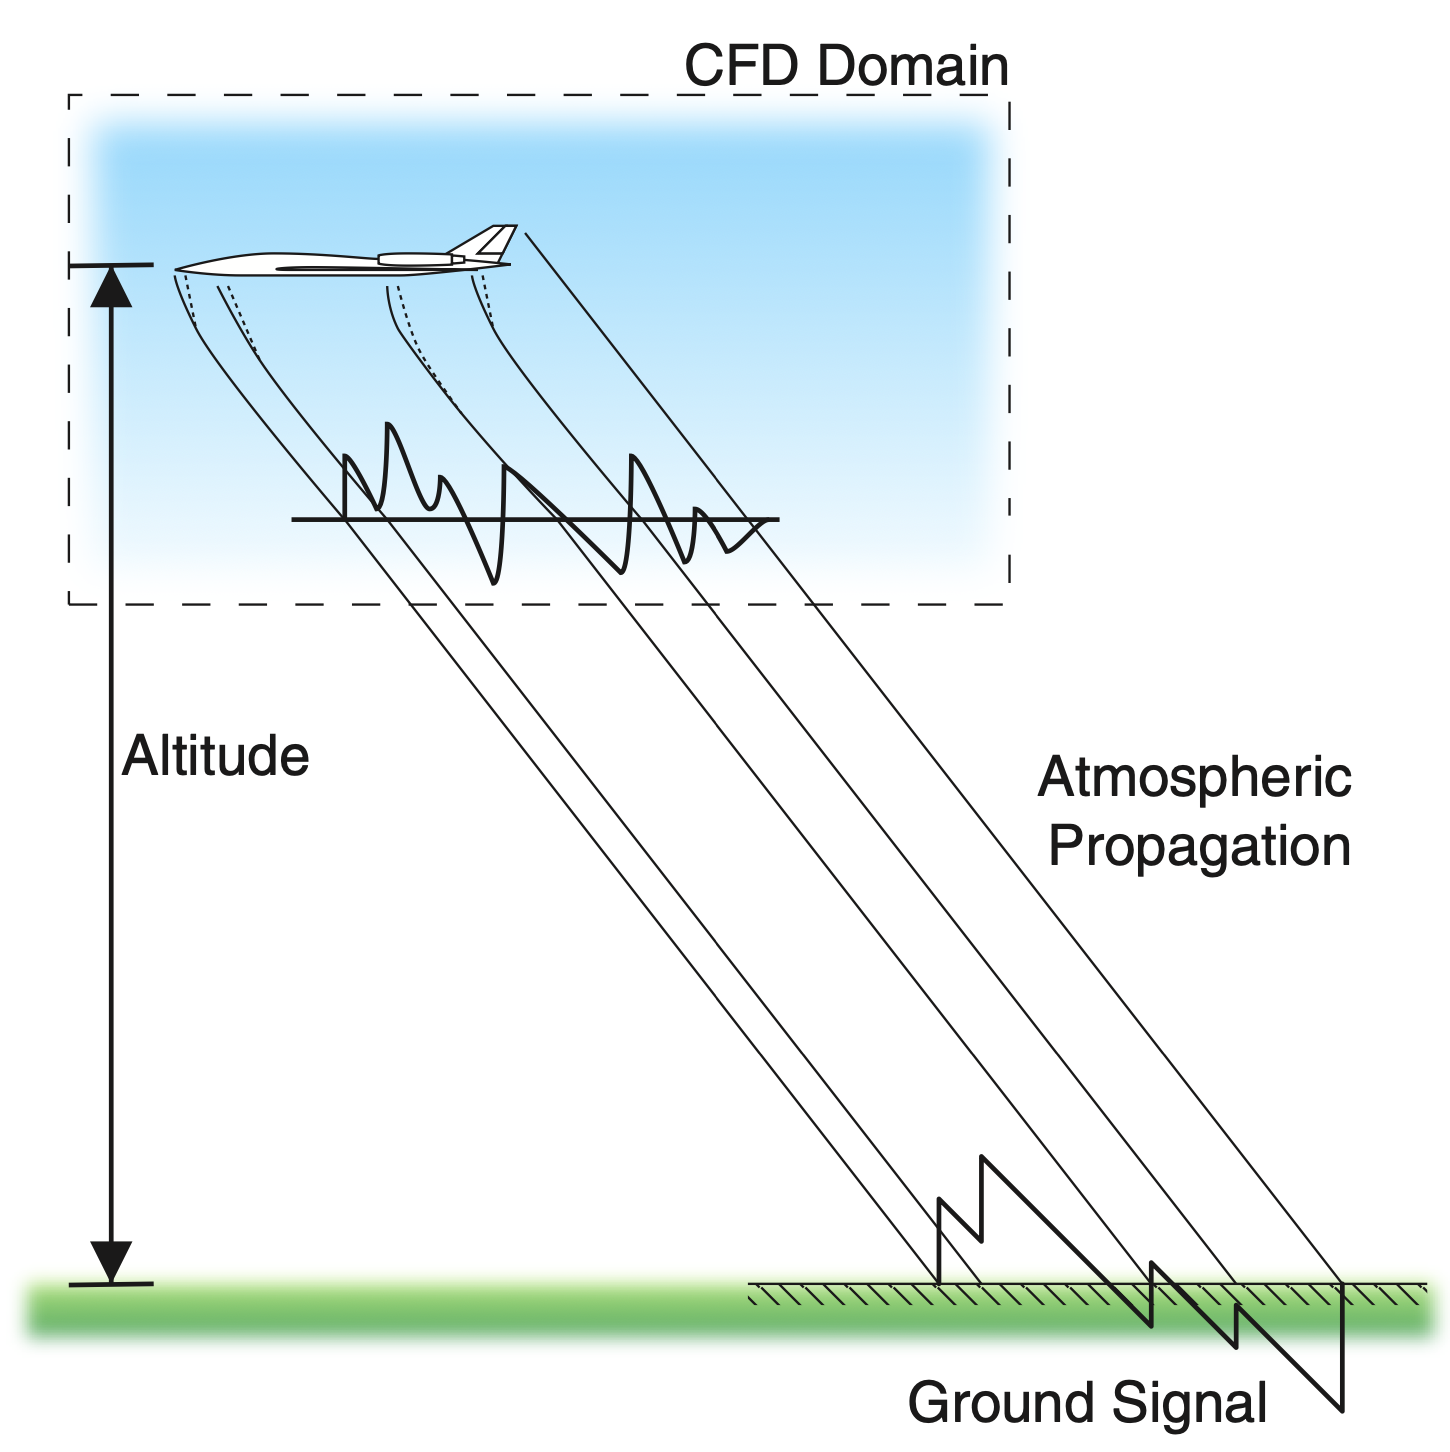
\includegraphics[height=5.5cm]{../figs/motivation/CFDandProp.png}};
      \end{scope}
  }

  \uncover<4->
  {
      % Overlay a copy of the image clipped to the region of interest (full opacity).
      \begin{scope}[remember picture,overlay]
        \node [anchor=north east, xshift=-0.2cm, yshift=-1.5cm]
        at (current page.north east) {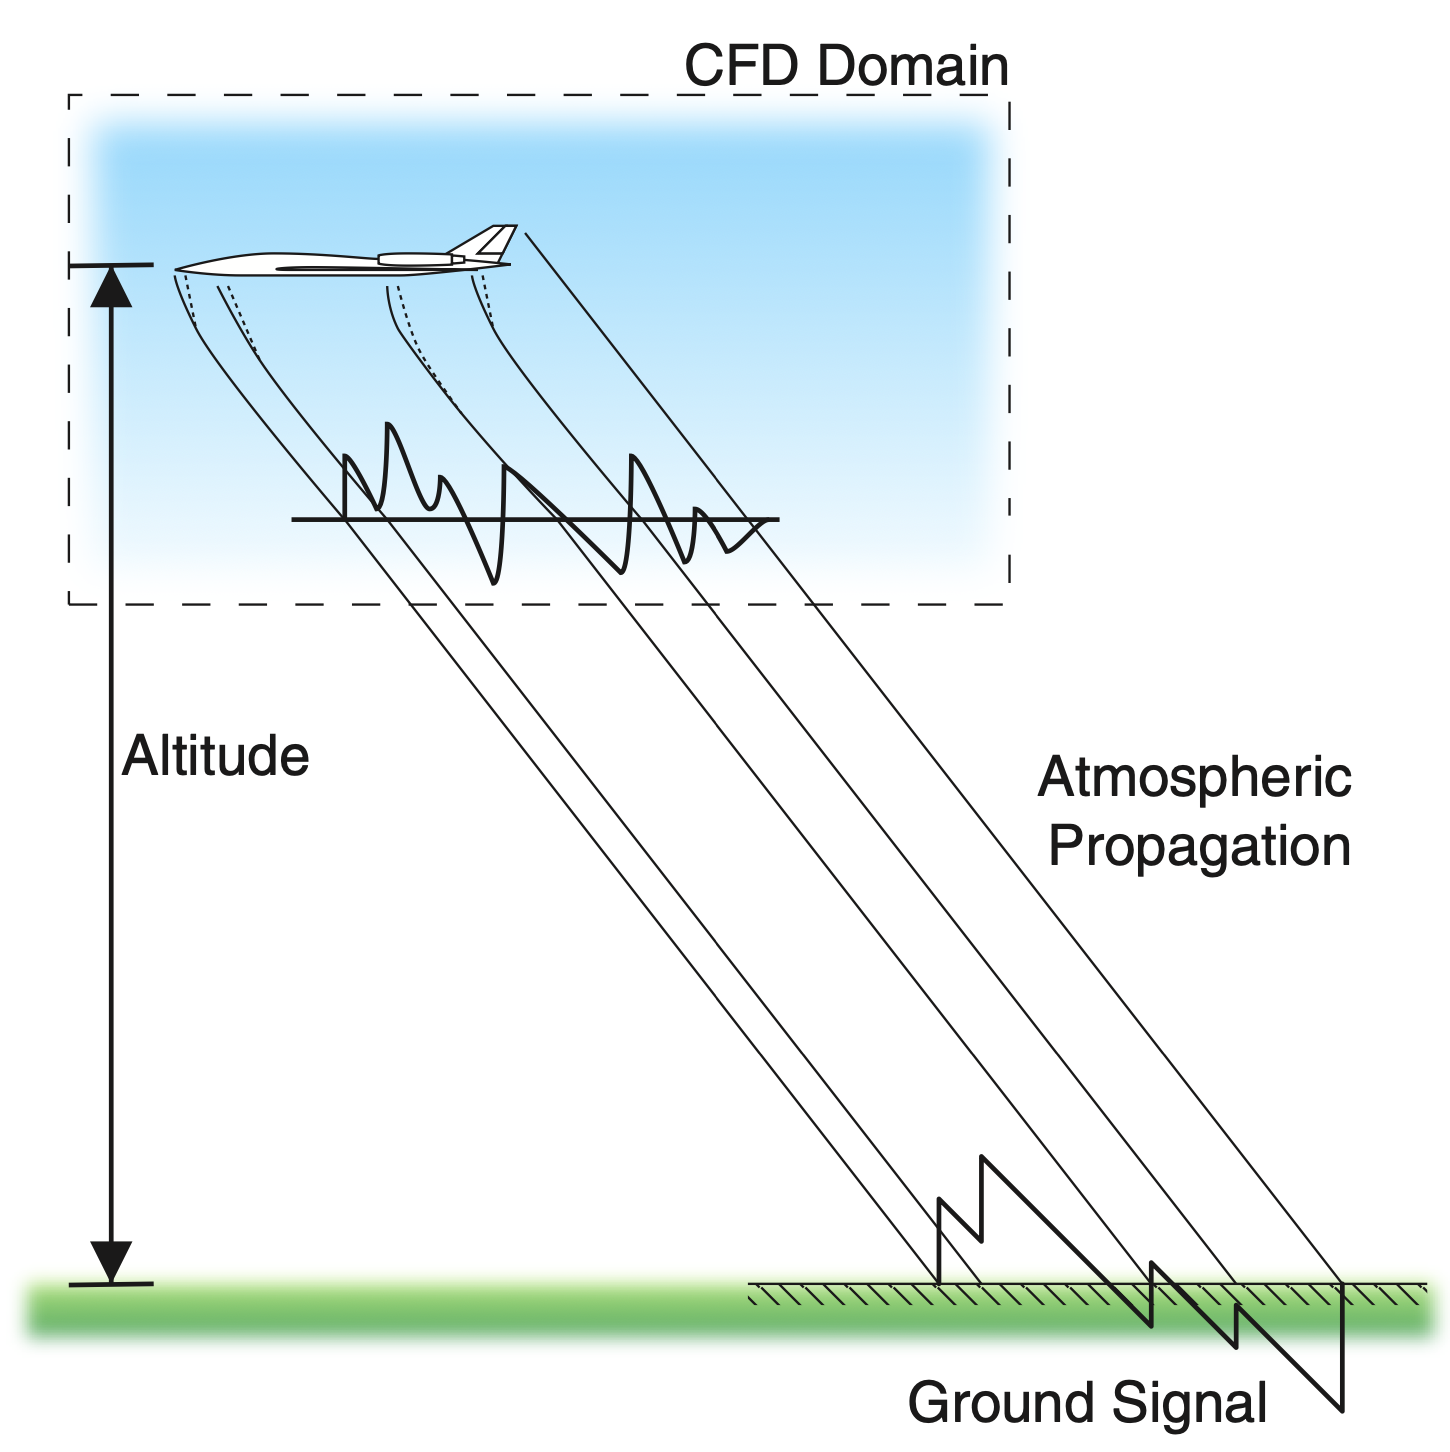
\includegraphics[height=5.5cm]{../figs/motivation/CFDandProp.png}};
      \end{scope}
  }

  \uncover<2->
  {
  \node[anchor=south west, font=\small, black, xshift=12mm, yshift=-11mm] at (img.north west) {$X$};
  }
    \uncover<3->
    {
    \node[anchor=south west, font=\small, black, xshift=31mm, yshift=-23mm] at (img.north west) {$p_{nf}$};
    }

    \uncover<4->
    {
      \begin{scope}[remember picture,overlay]
        % Draw an arrow
        \draw[->, black, thick]
          ($(img.north west)+(15mm,-25mm)$) -- ($(img.north west)+(19mm,-30mm)$);
      \end{scope}
    }

    \uncover<4->
    {
      \node[anchor=south west, font=\small, black, xshift=17.5mm, yshift=-34mm] at (img.north west) {$\sigma$};
    }

    \uncover<4->
    {
      \begin{scope}[remember picture,overlay]
        % Draw an arrow
        \draw[->, black, thick]
          ($(img.north west)+(20mm,-25.5mm)$) -- ($(img.north west)+(24.5mm,-25.5mm)$);
      \end{scope}
    }

    \uncover<4->
    {
      \node[anchor=south west, font=\small, black, xshift=22mm, yshift=-30mm] at (img.north west) {$\tau$};
    }

    \uncover<4->
    {
    \node[anchor=south west, font=\small, black, xshift=25mm, yshift=-50.5mm] at (img.north west) {Noise};
    }
  \end{tikzpicture}

  \uncover<6->
  {
  \begin{tikzpicture}[remember picture,overlay]
    \node[draw=red, dashed, thick, inner xsep=-5pt, inner ysep=4pt,
          fit=(start2) (end2), xshift=0mm, yshift=1mm] {};
  \end{tikzpicture}

  \begin{tikzpicture}[remember picture,overlay]
    \node[draw=red, dashed, thick, inner xsep=-50pt, inner ysep=13pt,
          fit=(start3) (end3), xshift=5.9mm, yshift=1.1mm] {};
  \end{tikzpicture}
  }

  \vspace{-55pt}\footnotetext{D. L. Rodriguez et. al. 2025}
\end{frame}

%---------------------------------------------------------------%

\stepcounter{sectionframecount}
\begin{frame}[t]{Propagation Problem: Motivation for Mesh Adaptation}

\textbf{Shock-dominated problem:} Need fine mesh in shock areas.

\uncover<2->
{
\begin{tikzpicture}[remember picture,overlay]
  \node[anchor=north east, xshift=-0.5cm, yshift=-2.3cm]
    at (current page.north east) {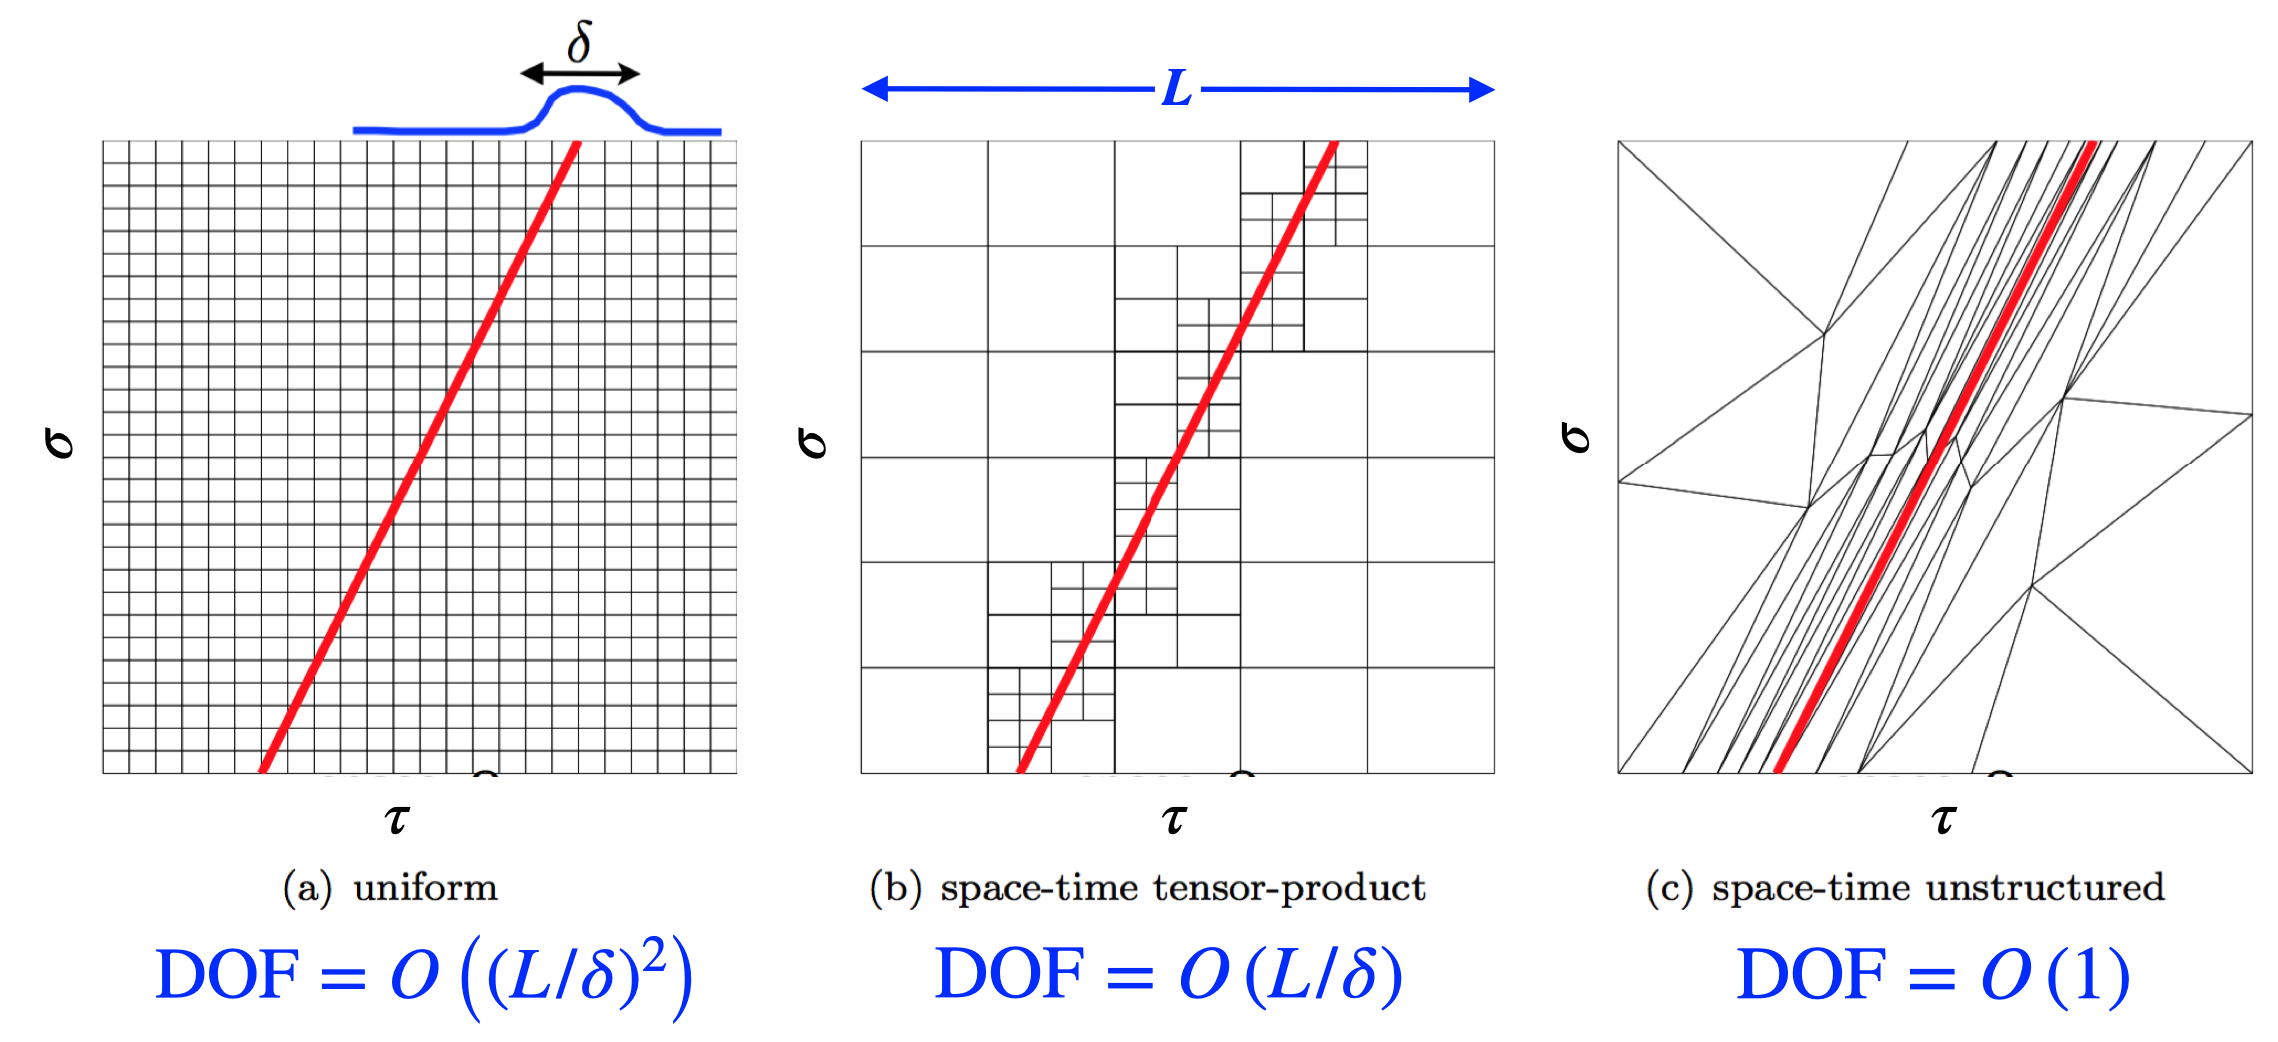
\includegraphics[height=5.5cm]{../figs/motivation/spaceTimeAdaptiveMethod.png}};

  % \node[anchor=south west, font=\tiny, black, xshift=-67mm, yshift=-9mm] at (img.north west) {Ground};

  % \node[anchor=south west, font=\tiny, black, xshift=-67mm, yshift=-46.5mm] at (img.north west) {Nearfield};
\end{tikzpicture}
}

\uncover<3->
{
\begin{minipage}[t]{1\linewidth}
  \vspace{4.9cm}
  But, space-time unstructured requires 2D solve instead of marching in $\sigma$.
\end{minipage}
}

\end{frame}

%---------------------------------------------------------------%

\stepcounter{sectionframecount}
\begin{frame}[t]{Propagation Problem: Motivation for Mesh Adaptation}
\vspace{-10pt}
\small \textbf{Target noise level at ground:} below 75 dB.

\small \textbf{Target noise error in simulations:} \textit{reliably} at order of 0.1 dB.
\uncover<2->
{
\vspace{-10pt}
\begin{minipage}[t]{1\linewidth}
  Results for standard time-marching methods\footnotemark:
\end{minipage}

\begin{tikzpicture}[remember picture,overlay]
  \node[anchor=north east, xshift=-4.5cm, yshift=-2.8cm] at (current page.north east) {%
    \begin{minipage}{0.5\textwidth}
    \scriptsize Approximate Error in Noise

    \end{minipage}
  };
\end{tikzpicture}

% \begin{tikzpicture}[remember picture,overlay]
%   \node[anchor=north east, xshift=0cm, yshift=-2.0cm] at (current page.north east) {%
%     \begin{minipage}{0.5\textwidth}
%     \small Error in $|d (\text{Noise})/d p_{nf}|$

%     \end{minipage}
%   };
% \end{tikzpicture}

\begin{tikzpicture}[remember picture,overlay]
  \node[anchor=north east, xshift=-6.1cm, yshift=-3.1cm]
    at (current page.north east) {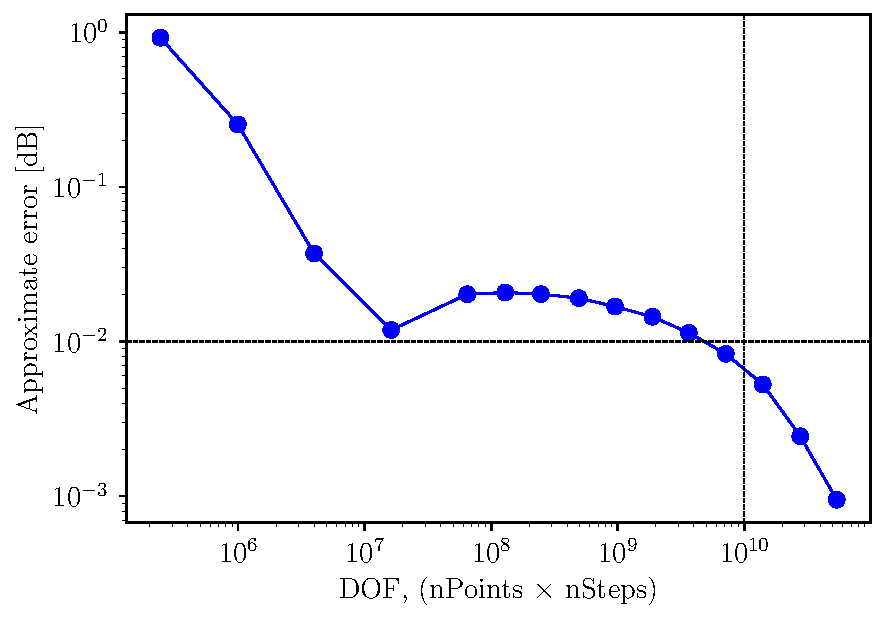
\includegraphics[height=4.25cm]{../figs/motivation/errorInNoisesBOOM.pdf}};
  \node[anchor=north east, xshift=-10.15cm, yshift=-6.35cm]
    at (current page.north east) {\tiny\color{gray} Source: [2]};
\end{tikzpicture}

% \begin{tikzpicture}[remember picture,overlay]
%   \node[anchor=north east, xshift=-1.5cm, yshift=-2.4cm]
%     at (current page.north east) {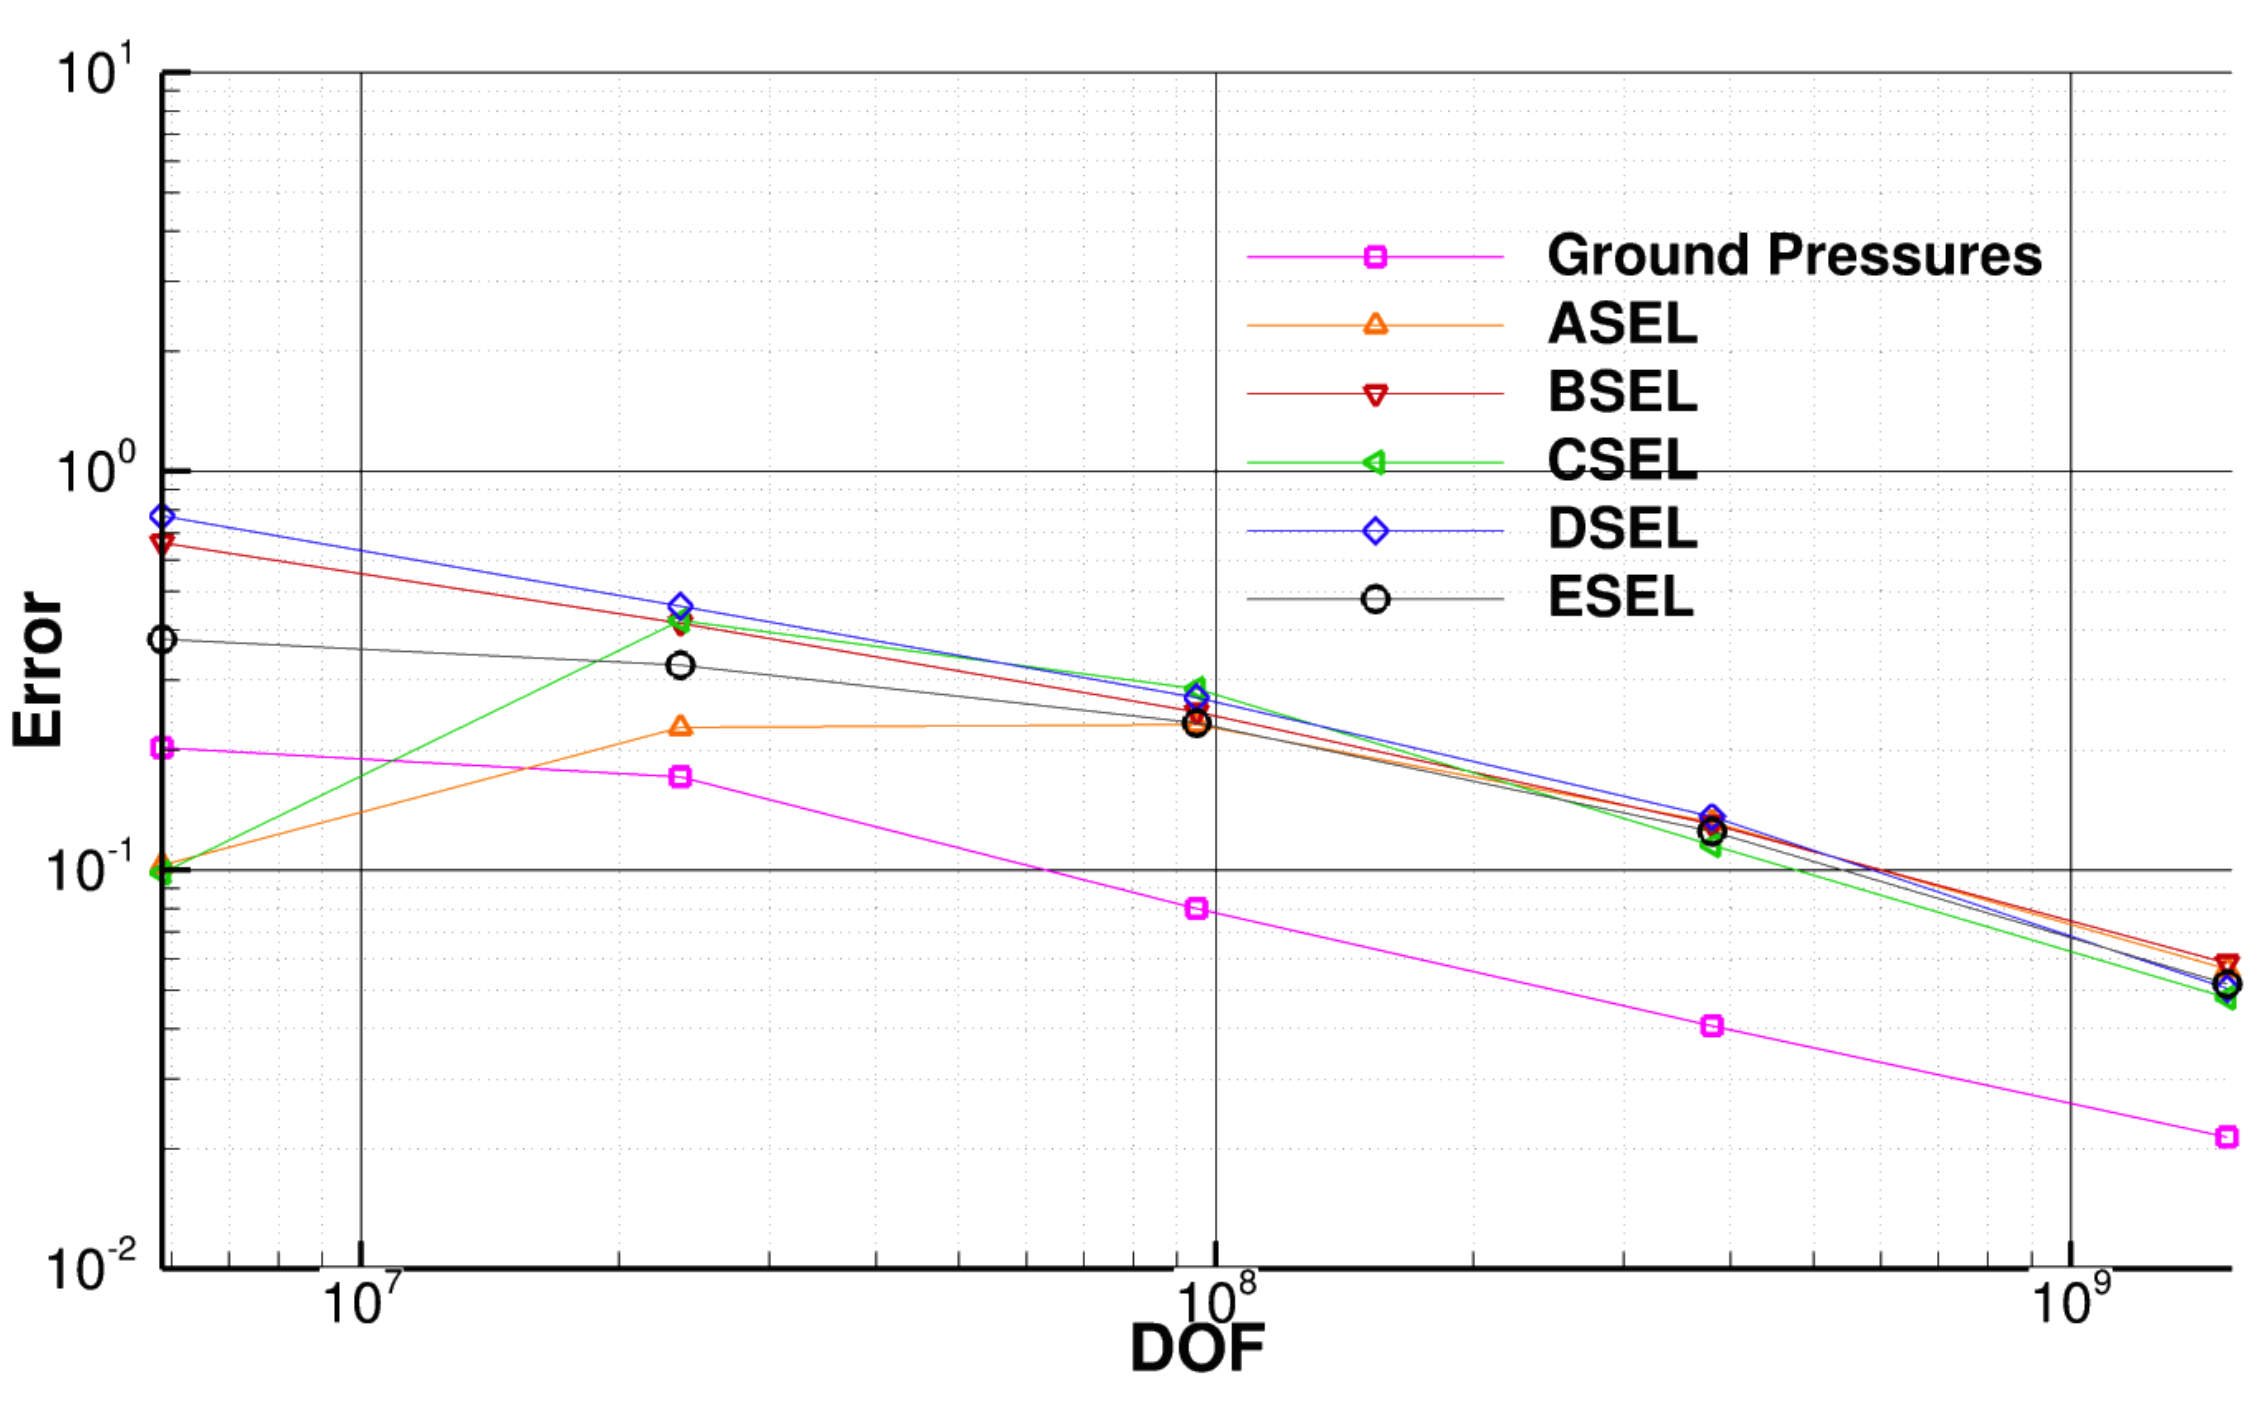
\includegraphics[height=3.5cm]{../figs/motivation/sensitivityNormErrorsBOOM.png}};
%   \node[anchor=north east, xshift=-5.5cm, yshift=-6cm]
%     at (current page.north east) {\tiny\color{gray} Source: [2]};
% \end{tikzpicture}

\begin{tikzpicture}[remember picture,overlay]
  \node[anchor=north east, xshift=0cm, yshift=-5.3cm] at (current page.north east) {%
    \begin{minipage}{0.5\textwidth}
    \scriptsize ($\approx 10^{10}$ DOF for $10^{-2}$ approx. error)

    \end{minipage}
  };
\end{tikzpicture}

% \begin{tikzpicture}[remember picture,overlay]
%   \node[anchor=north east, xshift=0cm, yshift=-6.4cm] at (current page.north east) {%
%     \begin{minipage}{0.5\textwidth}
%     \scriptsize ( $\approx 10^{10}$ DOF for $10^{-2}$ error )

%     \end{minipage}
%   };
% \end{tikzpicture}
}
\vspace{3.8cm}
\uncover<3->
{
\begin{minipage}[t]{1\linewidth}
  \textbf{Our goal:}
  Reduce the significant computational cost involved.

  Enable efficient, automated high accuracy predictions of boom propagation and design sensitivities through adaptive control of numerical error.
\end{minipage}
}

\vspace{-8pt}\footnotetext{S. K. Rallabhandi et. al. 2023}
\end{frame}

%=============================================================================%
%=============================================================================%
%=============================================================================%
% Section: Boom propagation modeling and Adaptive Approach

\begin{frame}[plain]
  \vfill
  \centering
  {\usebeamerfont{title}\usebeamercolor[fg]{title}Boom Propagation Modeling and Adaptive Approach}
  \vfill
\end{frame}

\section{Boom Propagation Modeling and Adaptive Approach}

\setsectionframes{3}

%---------------------------------------------------------------%

\stepcounter{sectionframecount}
\begin{frame}[t]{Coordinate System}
  \vspace{-8pt}
  Airplane at cruise altitude and cruise Mach number ($M_a$):

  \begin{tikzpicture}[remember picture,overlay]
    \node[anchor=north east, xshift=-1.1cm, yshift=-2.1cm]
    at (current page.north east) {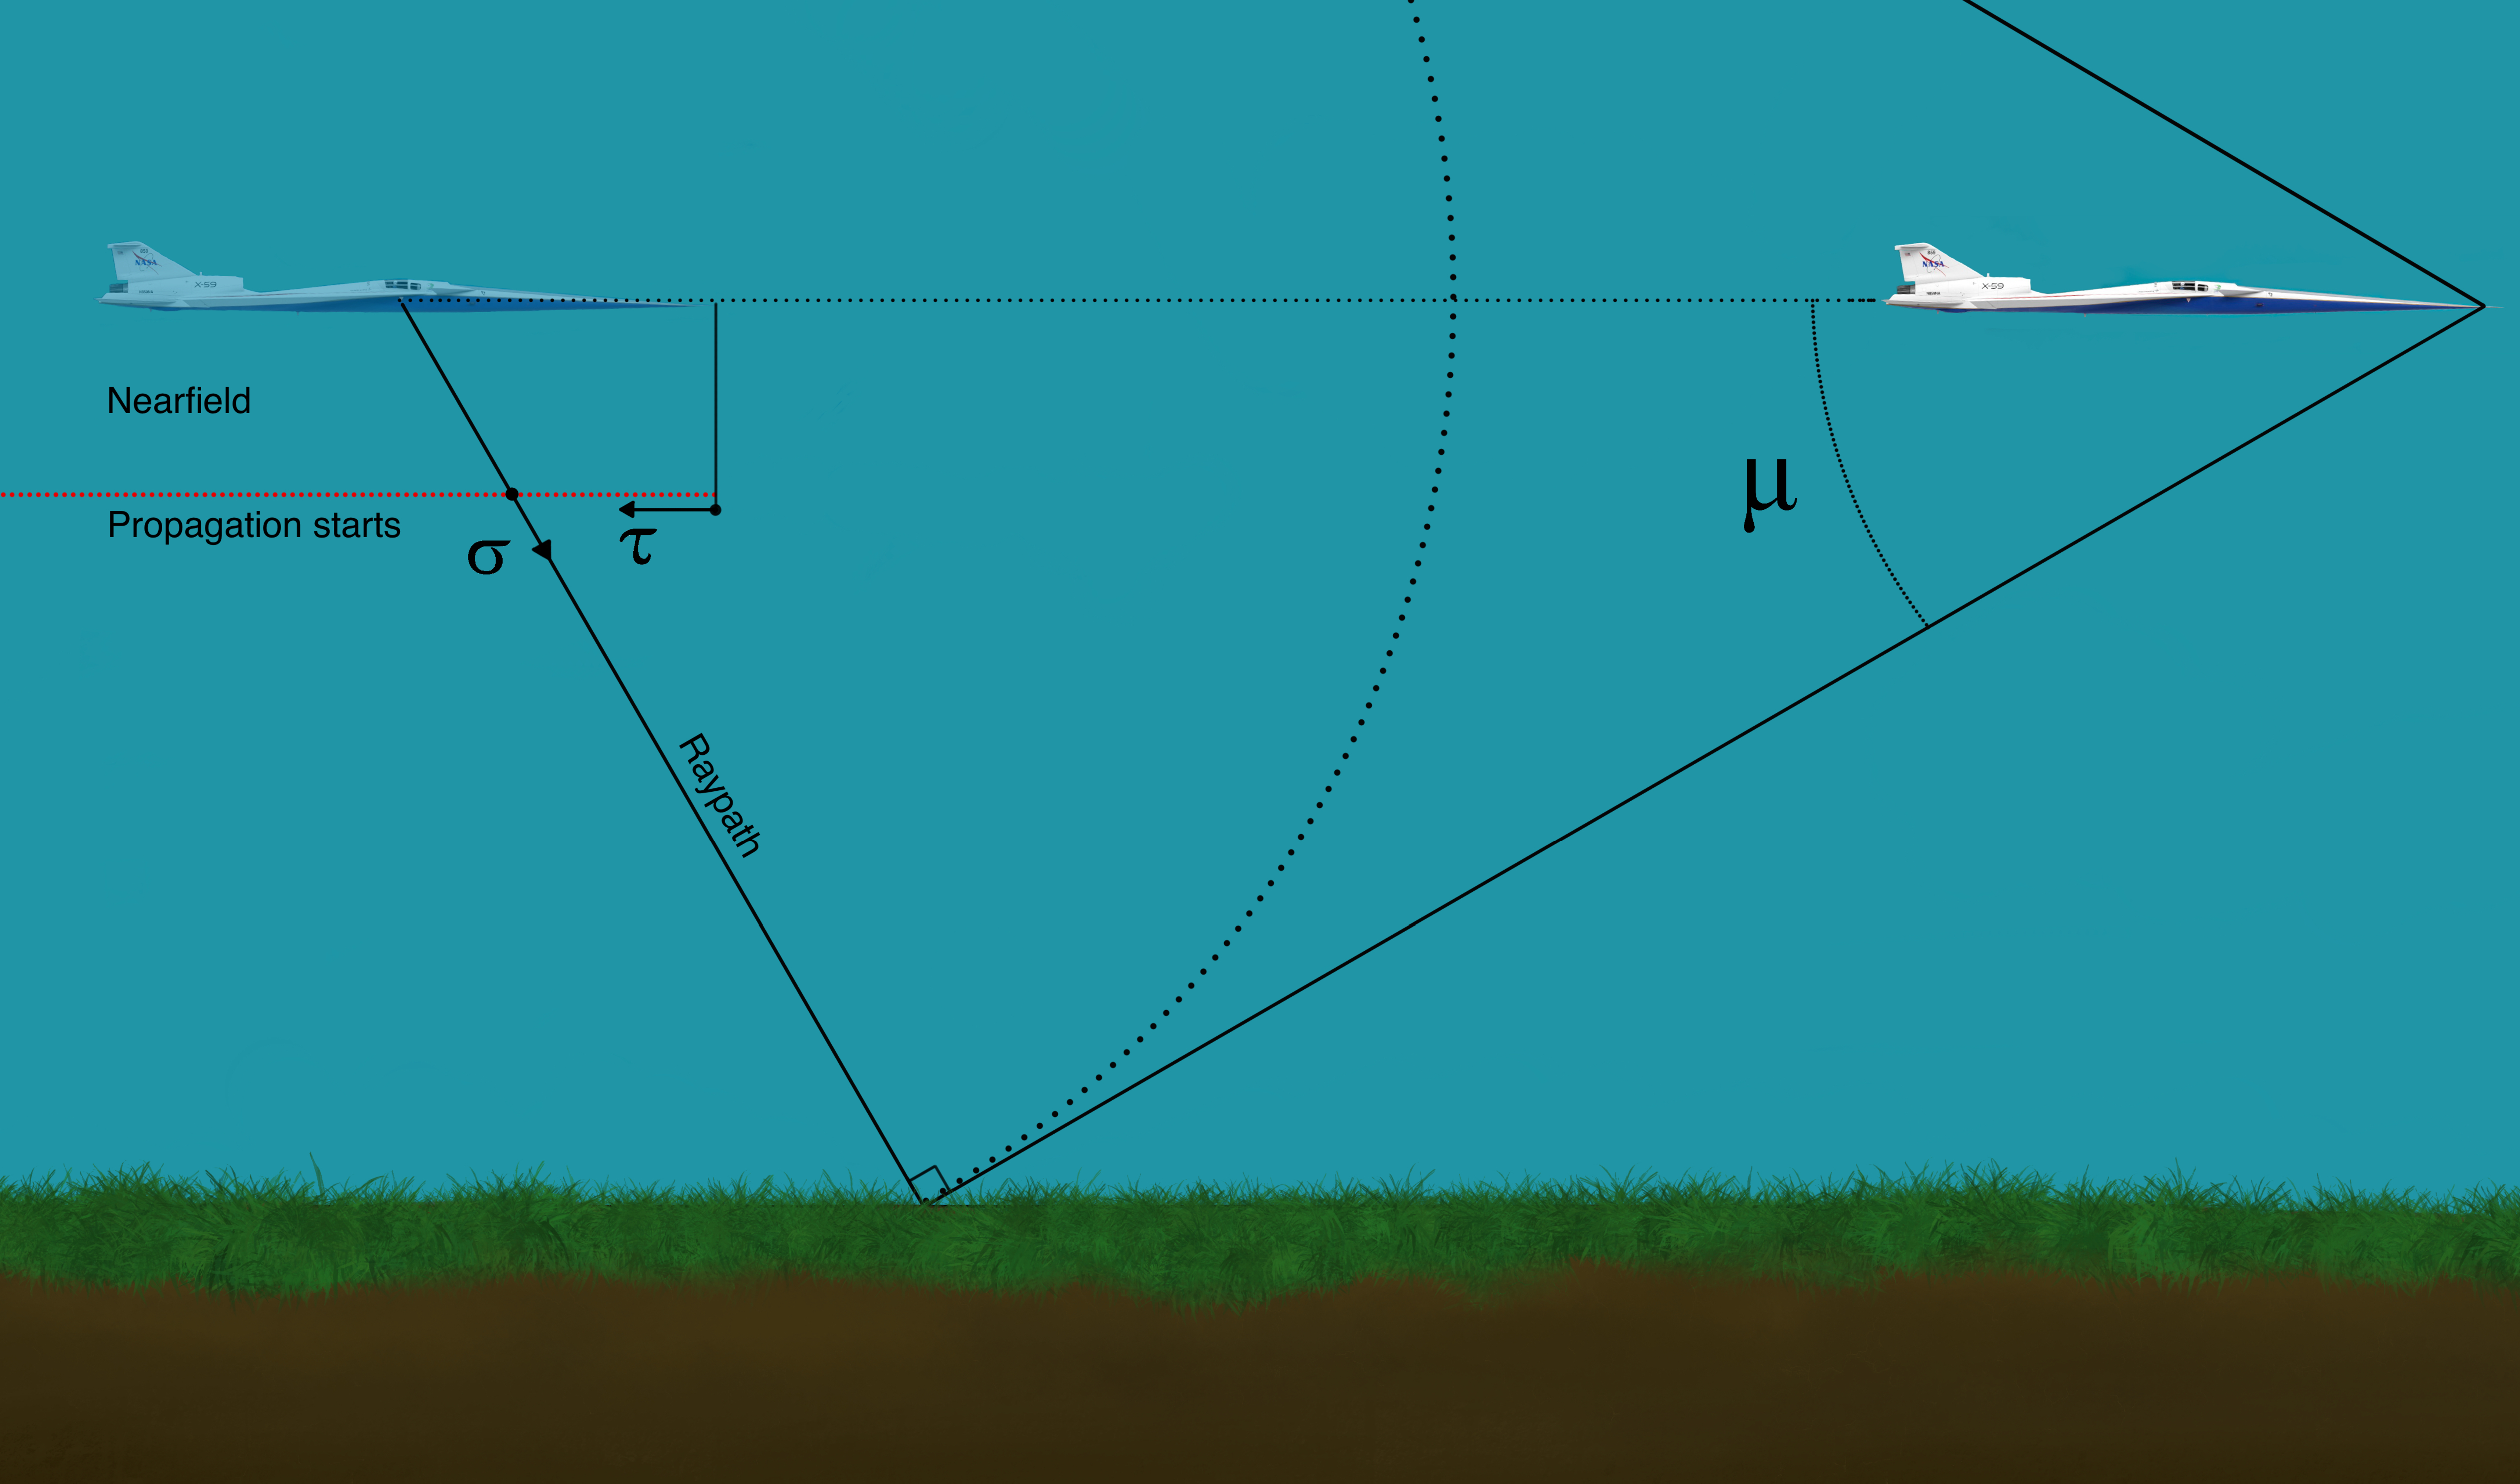
\includegraphics[height=6cm]{../figs/boom_modeling/Coordinate_System_.pdf}};
  \end{tikzpicture}

  \vspace{6cm}
  Mach cone angle: $\mu = \sin^{-1}(1/M_a)$.

\end{frame}

%---------------------------------------------------------------%

\stepcounter{sectionframecount}
\begin{frame}[t]{Augmented Burgers System}
  \vspace{-10pt}
  To model sonic boom propagation we use the augmented Burgers system of equations, for the states $(P, \tilde{P}_{\text{O}_2}, \tilde{P}_{\text{N}_2})$:

  \uncover<2->
  {
  \vspace{-10pt}
  \begin{equation}
    \small
    \dfrac{\partial P}{\partial \sigma}
    -\dfrac{1}{2}\dfrac{\partial \ln(\rho_0c_0/A_{n0})}{\partial \sigma}P
    -\dfrac{1}{2}\dfrac{\partial P^2}{\partial \tau}
    -\dfrac{1}{\Gamma}\dfrac{\partial ^2 P}{\partial \tau^2}
    -\dfrac{\partial }{\partial \tau}\left(\sum_{\nu} C_\nu \dfrac{\partial\tilde{P}_\nu}{\partial \tau}\right)
    =0\text{ on }\Omega,
    \label{e:augmented_burgers}
  \end{equation}

  \vspace{-3pt}
  \begin{equation}
    \small
    -\dfrac{\partial \tilde{P}_\nu}{\partial \tau} + \dfrac{P - \tilde{P}_\nu}{\theta_\nu} = 0\text{ on }\Omega,~~~~\nu = \{\text{O}_2,\text{N}_2\},
  \end{equation}
  which includes:
  \begin{itemize}
    \item Thermoviscous diffusion.
    \item Atmospheric absorption by relaxation species (O$_2$ and N$_2$).
    \item Ray tube area variation.
  \end{itemize}
  }

  \uncover<3->
  {
  \textbf{Remarks:}
  \begin{itemize}
    \item Eq (\ref{e:augmented_burgers}) is parabolic, with $\sigma$ the time-like direction.
    \item It is typically solved with a time-marching scheme. \textbf{Not in our case.}
  \end{itemize}
  }
\end{frame}

%---------------------------------------------------------------%

\stepcounter{sectionframecount}
\begin{frame}[t]{Output-based Adaptation Cycle}

  \vspace{5pt}
  \textbf{Adaptive cycle scheme:}

  \begin{tikzpicture}[remember picture,overlay]
    \node[anchor=north east, xshift=-0.1cm, yshift=-2.7cm]
    at (current page.north east) {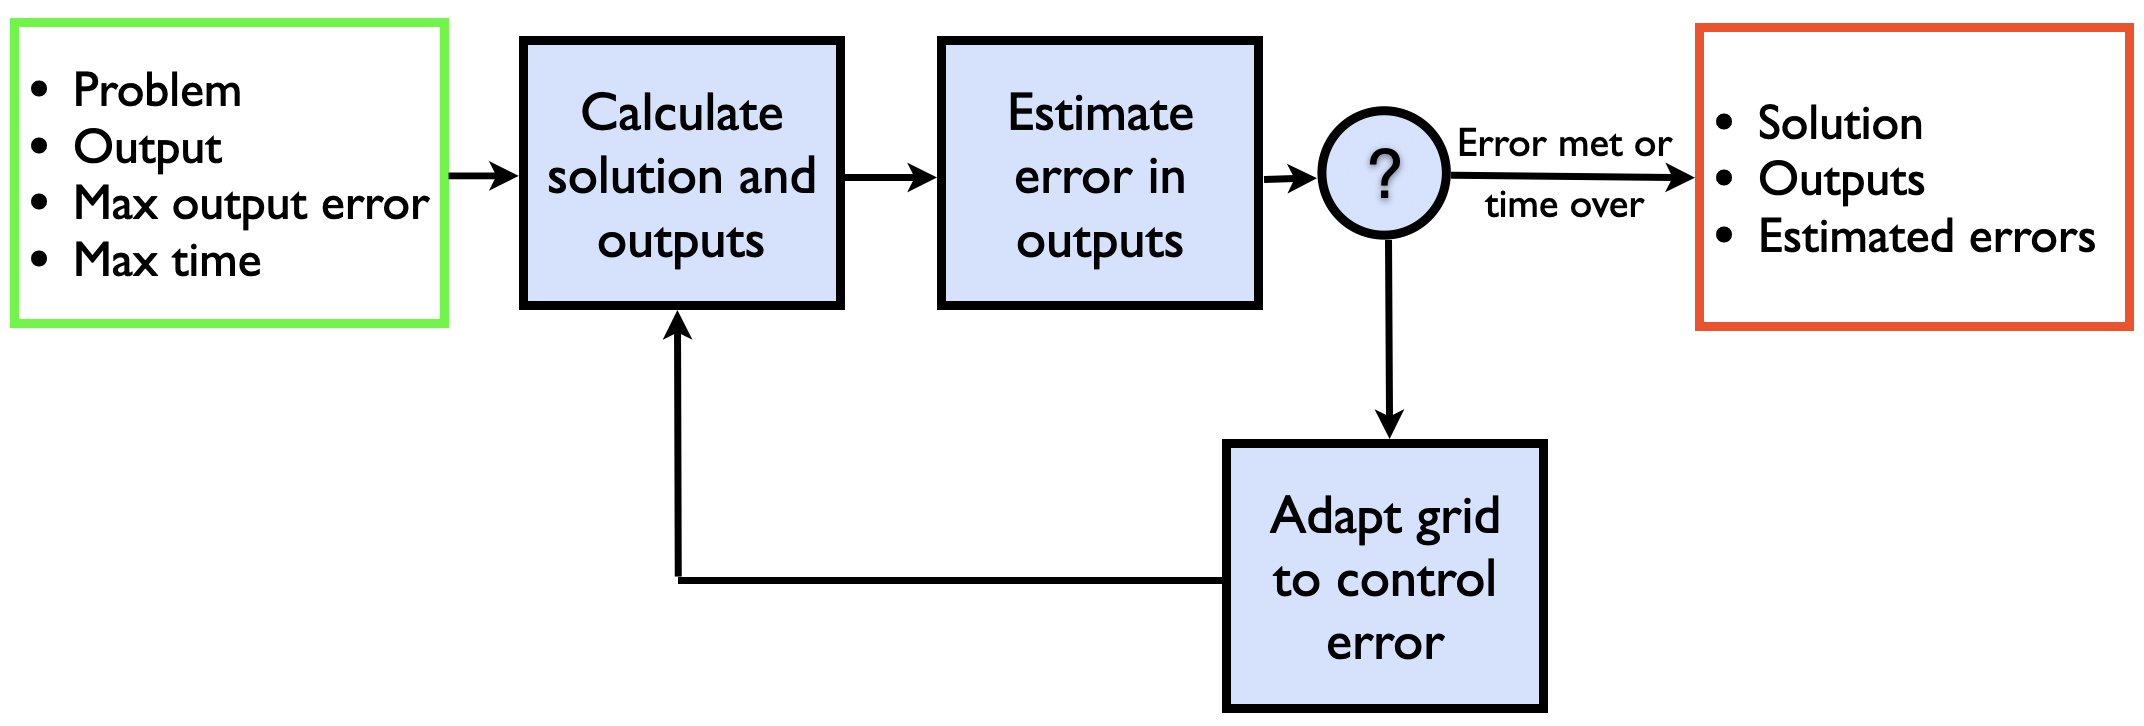
\includegraphics[height=4.2cm]{../figs/mesh_adaptation/adaptation_cycle.png}};
  \end{tikzpicture}

  \vspace{4.8cm}
  \textbf{Output of interest:} Loudness at ground.
\end{frame}

%=============================================================================%
%=============================================================================%
%=============================================================================%
% Section: Discretization and Shock capturing

\begin{frame}[plain, t]
  \vspace{2cm}
  \centering
  {\usebeamerfont{title}\usebeamercolor[fg]{title}Discretization and Shock Capturing}

  \begin{tikzpicture}[remember picture,overlay]
    % Place the full image (faded version)
    \node[anchor=north east, xshift=-0.6cm, yshift=-3.5cm, opacity=0.2] (img)
      at (current page.north east) {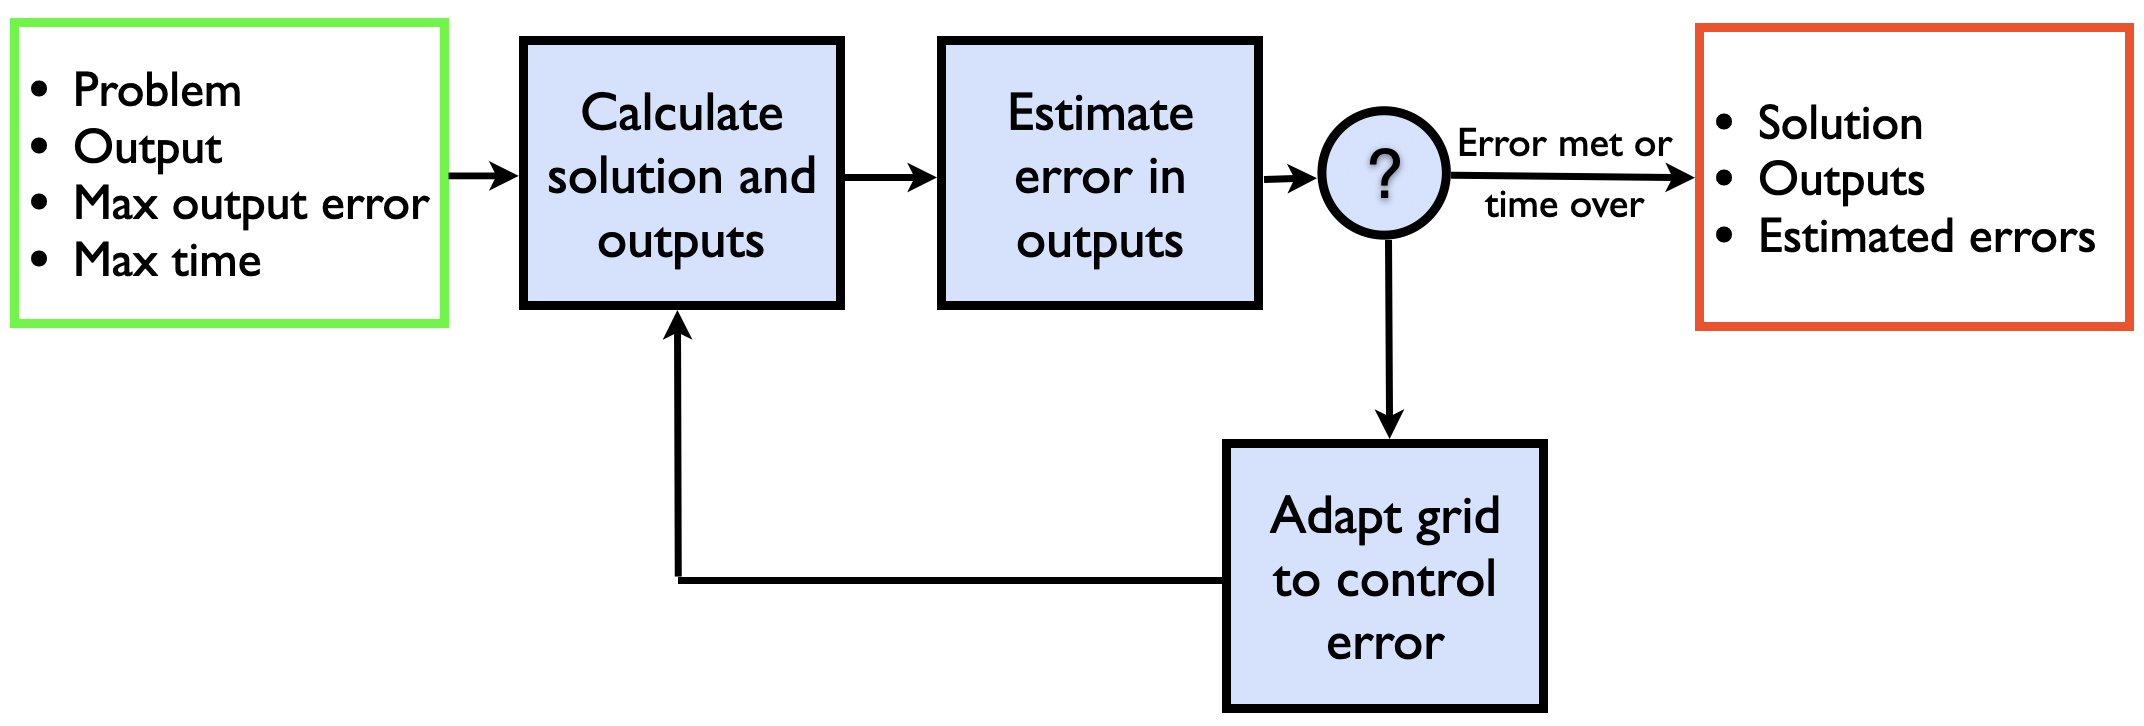
\includegraphics[height=3.8cm]{../figs/mesh_adaptation/adaptation_cycle.png}};

    % Define coordinates for the region to emphasize relative to the image node.
    % These coordinates are offsets from the image's north west corner.
    \coordinate (clipA) at ($(img.north west)+(2.8cm,-0.29cm)$);
    \coordinate (clipB) at ($(img.north west)+(4.6cm,-1.3cm)$);

    % Overlay a copy of the image clipped to the region of interest (full opacity).
    \begin{scope}[remember picture,overlay]
      \clip (clipA) rectangle (clipB);
      \node[anchor=north east, xshift=-0.6cm, yshift=-3.5cm]
        at (current page.north east) {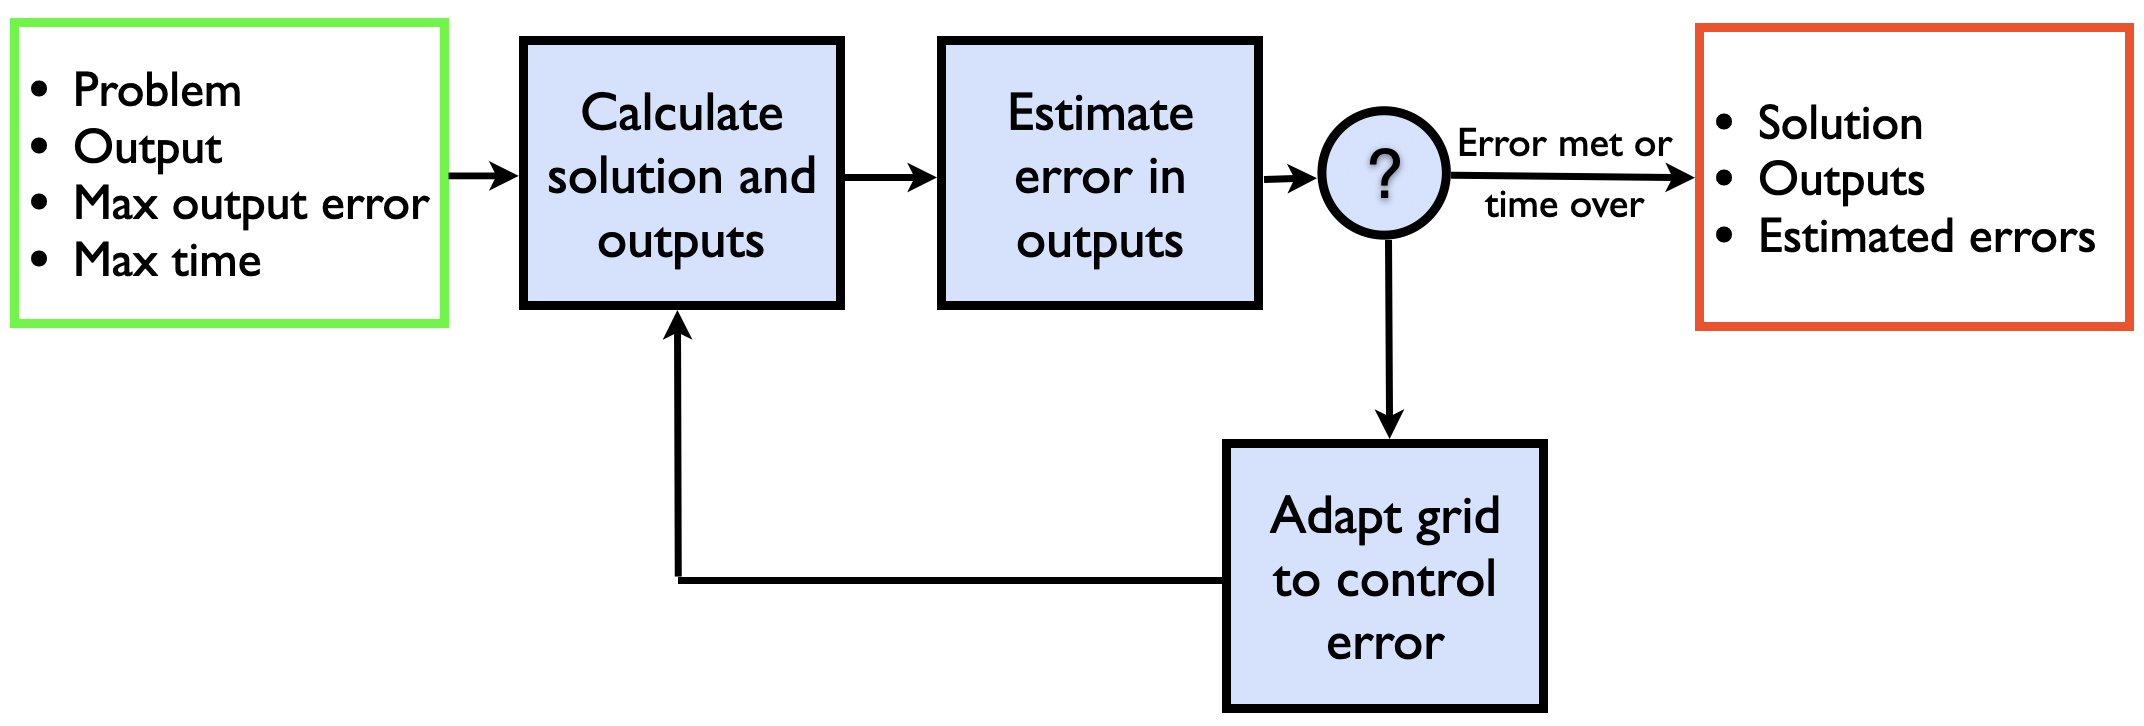
\includegraphics[height=3.8cm]{../figs/mesh_adaptation/adaptation_cycle.png}};
    \end{scope}

    % Draw a red dashed box around the highlighted region.
    \draw[red, dashed, thick] (clipA) rectangle (clipB);
  \end{tikzpicture}

\end{frame}

\section{Discretization and Shock Capturing}

\setsectionframes{5}

%---------------------------------------------------------------%

\stepcounter{sectionframecount}
\begin{frame}[t]{Continuous Galerkin type FEM}
  \textbf{CG weak statement:}

  \vspace{10pt}
  Find $\boldsymbol{u}_{h} \in \mathcal{V}_{h,p}$ such that:
  \begin{equation}
    \mathcal{R}(\boldsymbol{v}_{h},\boldsymbol{u}_{h}) = 0,~~\forall \boldsymbol{v}_{h} \in \mathcal{V}_{h,p},
    \label{e:multiscale_weak_statement}
  \end{equation}
  where the space $\mathcal{V}_{h,p}$ contains polynomials of order $p$ in $\Omega$.

  \uncover<2->
  {
  \vspace{10pt}
  \textbf{Remarks:}
  \begin{itemize}
    \item A discontinuous subscale is used for stabilization, and the resulting method is known as Variational Multiscale with Discontinuous Subscales (VMSD).
    \item The discretization is adjoint consistent.
  \end{itemize}
  }

\end{frame}

%---------------------------------------------------------------%

\stepcounter{sectionframecount}
\begin{frame}[t]{The Need for Artificial Viscosity}
\vspace{-10pt}
\textbf{Challenge:} Discontinuities (shocks) in the solutions, leading to unstable
numerical solves and lack of convergence.

\uncover<2->
{
\vspace{5pt}
\textbf{Goal:} Smoothen discontinuities to improve stability, while not modifying
the already smooth areas.
}

\uncover<3->{
\vspace{5pt}
\textbf{Approach:} Employ a shock sensor, $s$, to keep track of discontinuities, and use that information to add localized artificial viscosity.
}

\uncover<4->
{
\vspace{10pt}
Add extra diffusion term in Burgers equation:
\vspace{-2pt}
\begin{equation}
  \footnotesize
  \dfrac{\partial P}{\partial \sigma}
  -\dfrac{1}{2}\dfrac{\partial \ln(\rho_0c_0/A_{n0})}{\partial \sigma}P
  -\dfrac{1}{2}\dfrac{\partial P^2}{\partial \tau}
  -\dfrac{1}{\Gamma}\dfrac{\partial ^2 P}{\partial \tau^2}
  -\dfrac{\partial }{\partial \tau}\left(\sum_{\nu} C_\nu \dfrac{\partial\tilde{P}_\nu}{\partial \tau}\right)
  \underbrace{- \dfrac{\partial}{\partial \tau} \left(\epsilon_{\text{AV}}\dfrac{\partial P}{\partial \tau}\right)}_{\text{extra term}}
  =0,
\end{equation}
with $\epsilon_{\text{AV}}$ as:
\vspace{-2pt}
\begin{equation}
  \footnotesize
  \epsilon_{\text{AV}} := \underbrace{\dfrac{1}{2}\dfrac{H_{\tau\tau}}{p}|P|}_{\text{AV}_{\text{max}}}s.
\end{equation}
}

\end{frame}

%---------------------------------------------------------------%

\stepcounter{sectionframecount}
\begin{frame}[t]{PDE-based Shock Sensor\footnotemark}
\vspace{-10pt}

\textbf{Shock sensor design requirements:}
\begin{itemize}
    \item $s \approx 1$ in shock areas.
    \item $s \approx 0$ away from shocks.
    \item $s$ smooth.
\end{itemize}
\uncover<2->
{
\textbf{Define PDE for shock sensor $s$:}
\begin{equation}
  \underbrace{s - C_1s_{\text{grad}}}_{\text{source term}}} \uncover<3->{+ \underbrace{C_2\nabla \cdot \left(\dfrac{H^TH}{p^2} \nabla s\right)}_{\text{diffusion term}}} \uncover<2->{= 0\text{ on }\Omega.}
	\label{e:sensor_source}
\end{equation}

\begin{itemize}
  \uncover<2->
  {
  \item $s_{\text{grad}}$: \textbf{Shock indicator} based on pressure solution gradient.
  }

  \uncover<3->
  {
  \item Diffusion term: to have a smooth sensor solution.
  \item $H$: element size field.
  }

\end{itemize}

\footnotetext{G. E. Barter and D. L. Darmofal 2007}
\end{frame}

%---------------------------------------------------------------%

\stepcounter{sectionframecount}
\begin{frame}[t]{Shock Indicator $s_{\text{grad}}$}
  \vspace{-10pt}
  Identify pressure changes in $\tau$ direction:
  \begin{equation}
    \xi := \dfrac{H_{\tau\tau}}{p} \left|\dfrac{\partial P}{\partial \tau}\right|,~~~\hat{\xi} := \dfrac{\xi}{\xi_1},
  \end{equation}

  \uncover<2->
  {
  \begin{tikzpicture}[remember picture,overlay]
    \node[anchor=north east, xshift=0cm, yshift=-3.4cm]
    at (current page.north east) {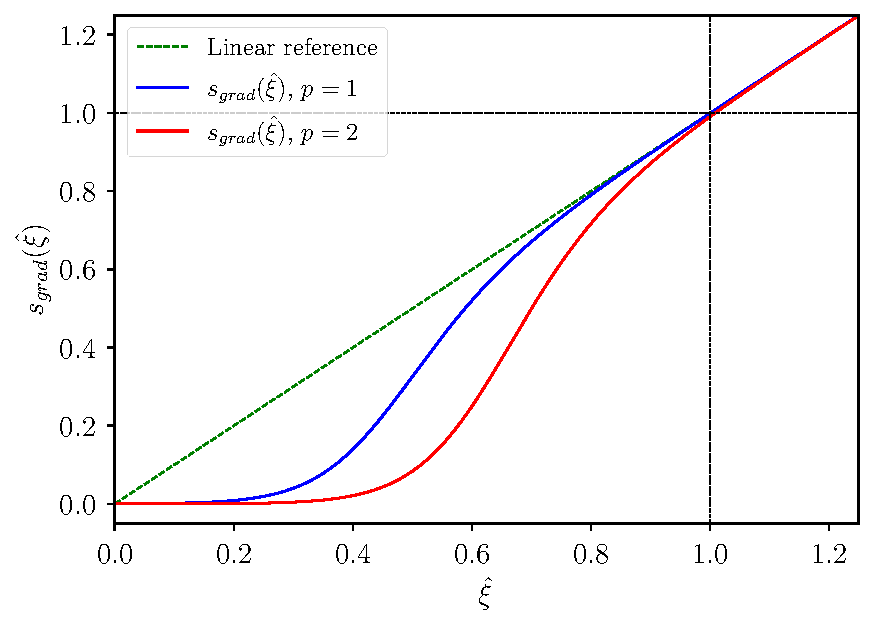
\includegraphics[height=5.7cm]{../figs/shock_capturing/s_grad.pdf}};
  \end{tikzpicture}

  \begin{tikzpicture}[remember picture,overlay]
    \node[anchor=north east, xshift=-7.7cm, yshift=-3.6cm] at (current page.north east) {%
      \begin{minipage}{0.4\textwidth}
        Define $s_{grad}(\hat{\xi})$ to meet design requirements
      \end{minipage}
    };
  \end{tikzpicture}
  }
\end{frame}


%---------------------------------------------------------------%

\stepcounter{sectionframecount}
\begin{frame}[t]{Test With Smooth Problem}
\vspace{-10pt}
Smooth problem with available exact solution:

\begin{itemize}
  \item Solve without artificial viscosity.
  \item Solve with artificial viscosity and see how it affects convergence.
\end{itemize}

\uncover<2->
{
\begin{tikzpicture}[remember picture,overlay]

  \node[anchor=north east, xshift=-2.75cm, yshift=-3.2cm] at (current page.north east) {%
    \begin{minipage}{0.5\textwidth}
    \small Output error for adaptive refinement

    \end{minipage}
  };
\end{tikzpicture}

\begin{tikzpicture}[remember picture,overlay]
  \node[anchor=north east, xshift=-2.6cm, yshift=-3.5cm]
  at (current page.north east) {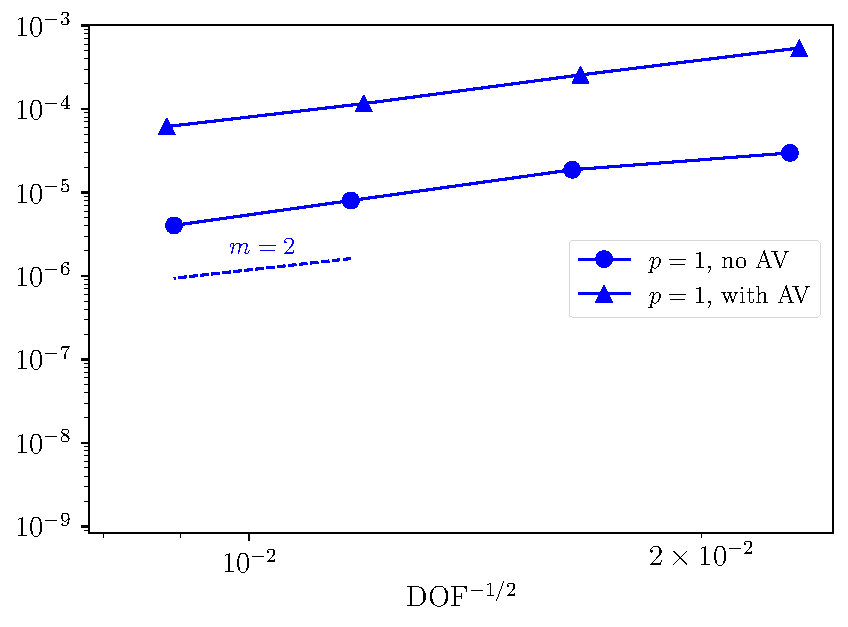
\includegraphics[height=5.5cm]{../figs/shock_capturing/outputErrorP1only.pdf}};
\end{tikzpicture}
}

\uncover<3->
{
  \begin{tikzpicture}[remember picture,overlay]
    \node[anchor=north east, xshift=-2.6cm, yshift=-3.5cm]
    at (current page.north east) {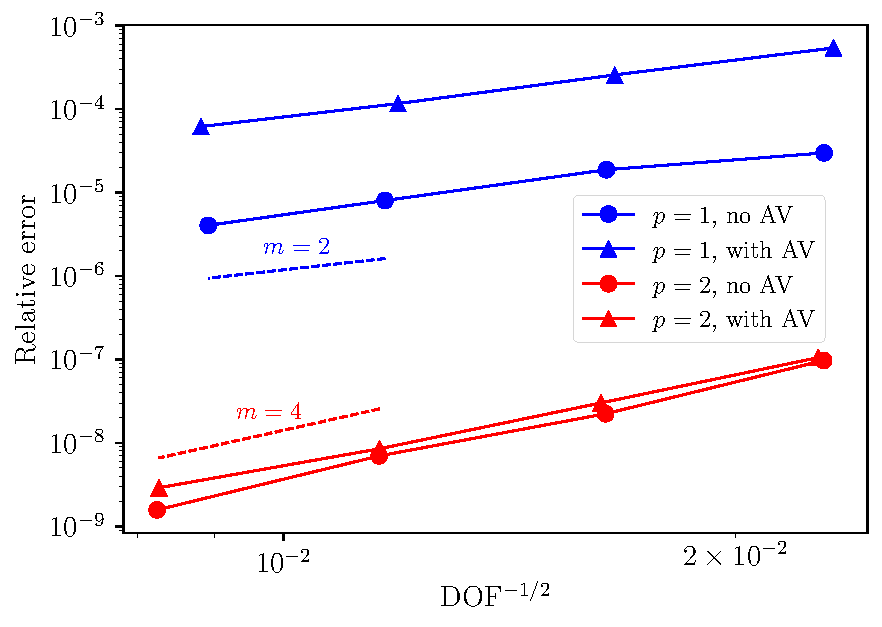
\includegraphics[height=5.5cm]{../figs/shock_capturing/outputError.pdf}};
  \end{tikzpicture}
}
\end{frame}

%=============================================================================%
%=============================================================================%
%=============================================================================%
% Section: Ground signal filtering

\begin{frame}[plain, t]
  \vspace{2cm}
  \centering
  {\usebeamerfont{title}\usebeamercolor[fg]{title}Ground Signal Filtering}

  \begin{tikzpicture}[remember picture,overlay]
    % Place the full image (faded version)
    \node[anchor=north east, xshift=-0.6cm, yshift=-3.5cm, opacity=0.2] (img)
      at (current page.north east) {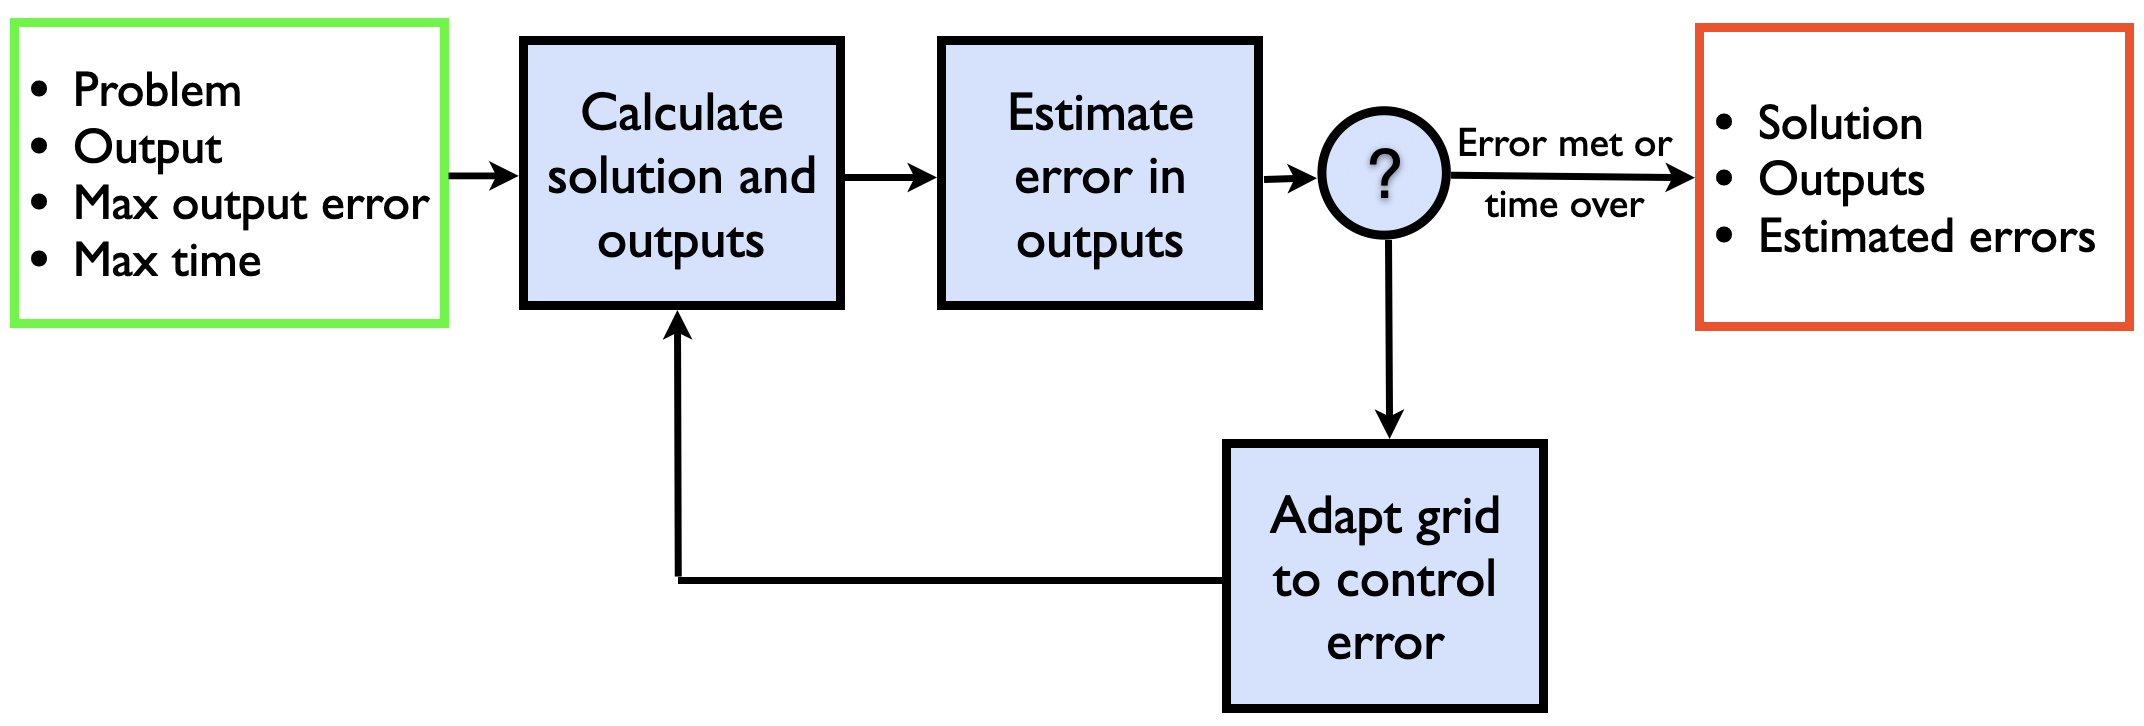
\includegraphics[height=3.8cm]{../figs/mesh_adaptation/adaptation_cycle.png}};

    % Define coordinates for the region to emphasize relative to the image node.
    % These coordinates are offsets from the image's north west corner.
    \coordinate (clipA) at ($(img.north west)+(2.8cm,-1.2cm)$);
    \coordinate (clipB) at ($(img.north west)+(4.6cm,-1.7cm)$);

    % Overlay a copy of the image clipped to the region of interest (full opacity).
    \begin{scope}[remember picture,overlay]
      \clip (clipA) rectangle (clipB);
      \node[anchor=north east, xshift=-0.6cm, yshift=-3.5cm]
        at (current page.north east) {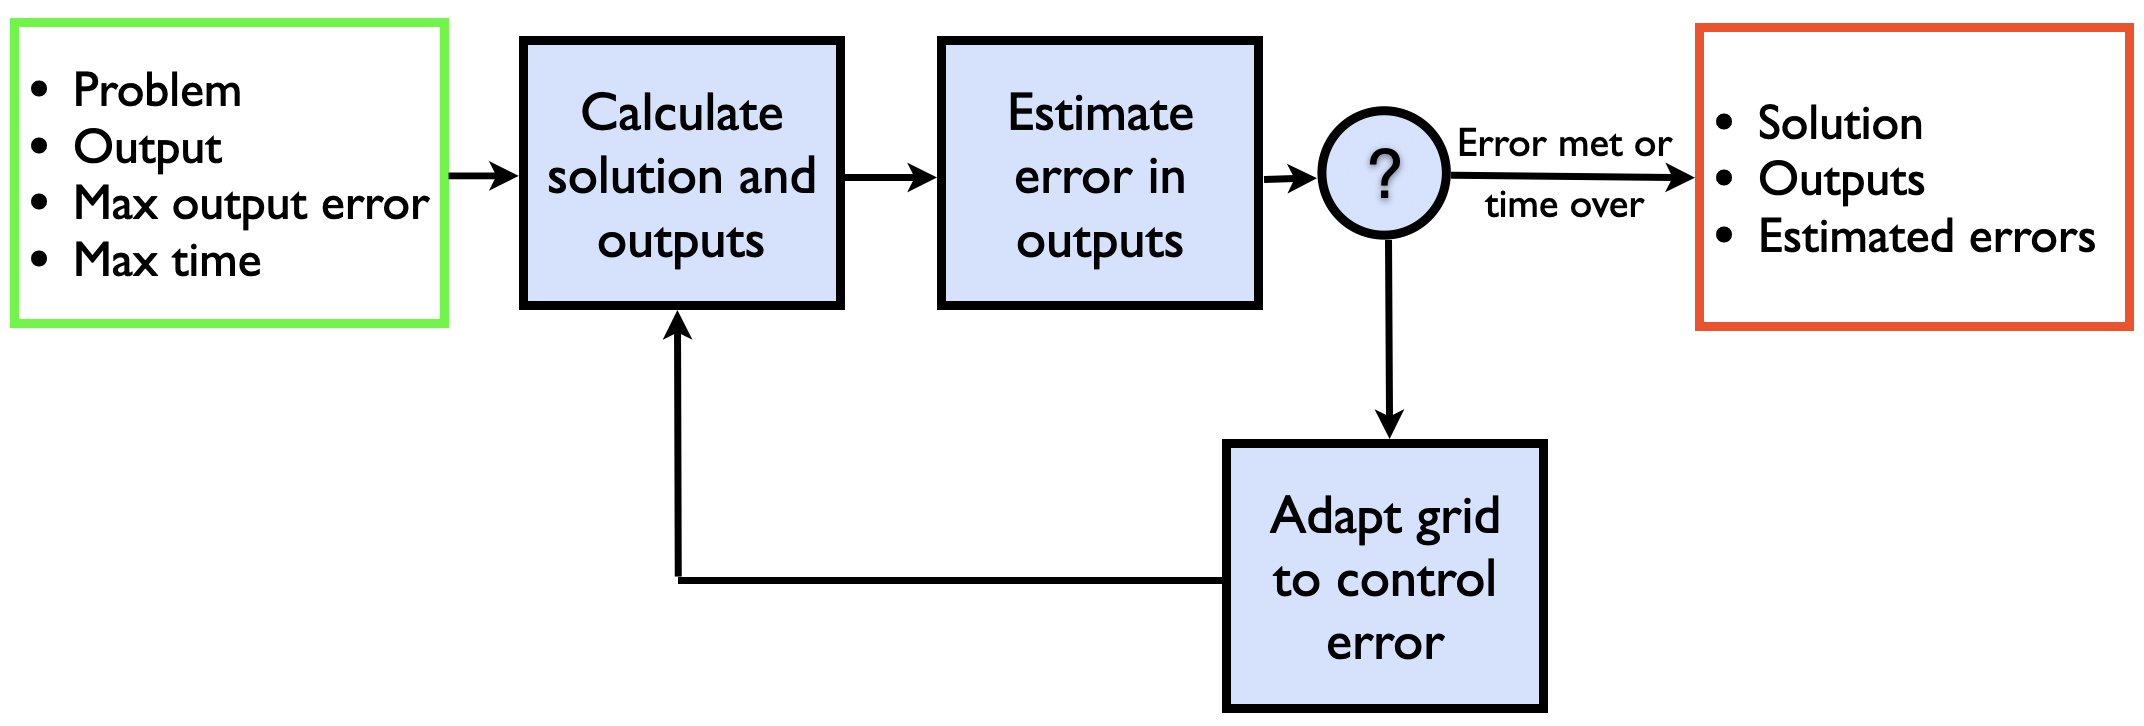
\includegraphics[height=3.8cm]{../figs/mesh_adaptation/adaptation_cycle.png}};
    \end{scope}

    % Draw a red dashed box around the highlighted region.
    \draw[red, dashed, thick] (clipA) rectangle (clipB);
  \end{tikzpicture}

\end{frame}

\section{Ground Signal Filtering}

\setsectionframes{3}

%---------------------------------------------------------------%

\stepcounter{sectionframecount}
\begin{frame}[t]{At Ground: Relevant Loudness Metrics}
\vspace{-10pt}
The human ear is less sensitive to low audio frequencies.

\vspace{10pt}
There is a family of weighting filter curves that account for this relative loudness perceived by humans: A/B/C/D/-SEL curves.

\uncover<2->
{
\vspace{10pt}
$\underbrace{p(\tau)}_{\text{Ground pressure signal}}\to~~~\text{Weighting filter}~~~\to\underbrace{\tilde{p}(\tau)}_{\text{Filtered signal}}$
}

\uncover<3->
{
\vspace{10pt}
Sound exposure:

\begin{equation}
  E = \dfrac{1}{\omega_{\text{ref}}}\int_{\tau_0}^{\tau_{\text{f}}} [\tilde{p}(\tau)]^2~d\tau.
\end{equation}
}

\uncover<4->
{
\vspace{4pt}
Loudness level in dB:

\begin{equation}
  \text{Loudness} = 10\log_{10}\left(\dfrac{E}{E_0}\right),~~~ E_0 = 400~ (\mu\text{Pa})^2s.
\end{equation}
}

\end{frame}

%---------------------------------------------------------------%

\stepcounter{sectionframecount}
\begin{frame}[t]{B-SEL Metric}
\vspace{-10pt}
We focus on the B-SEL curve, and the approach can be generalized to any other.

\uncover<2->
{
\vspace{4pt}
Transfer function in the complex frequency ($\chi$) domain:
\vspace{-5pt}
\begin{equation}
  \small
  H_B(\chi) =\dfrac{\tilde{P}(\chi)}{P(\chi)} = \dfrac{c_B \chi^3}{(\chi+2\pi f_1)^2(\chi+2\pi f_{2B})(\chi+2\pi f_4)^2},
  \label{e:continuous_transfer}
\end{equation}
}

\uncover<3->
{
\begin{tikzpicture}[remember picture,overlay]
  \node[anchor=north east, xshift=-1.1cm, yshift=-4.1cm]
  at (current page.north east) {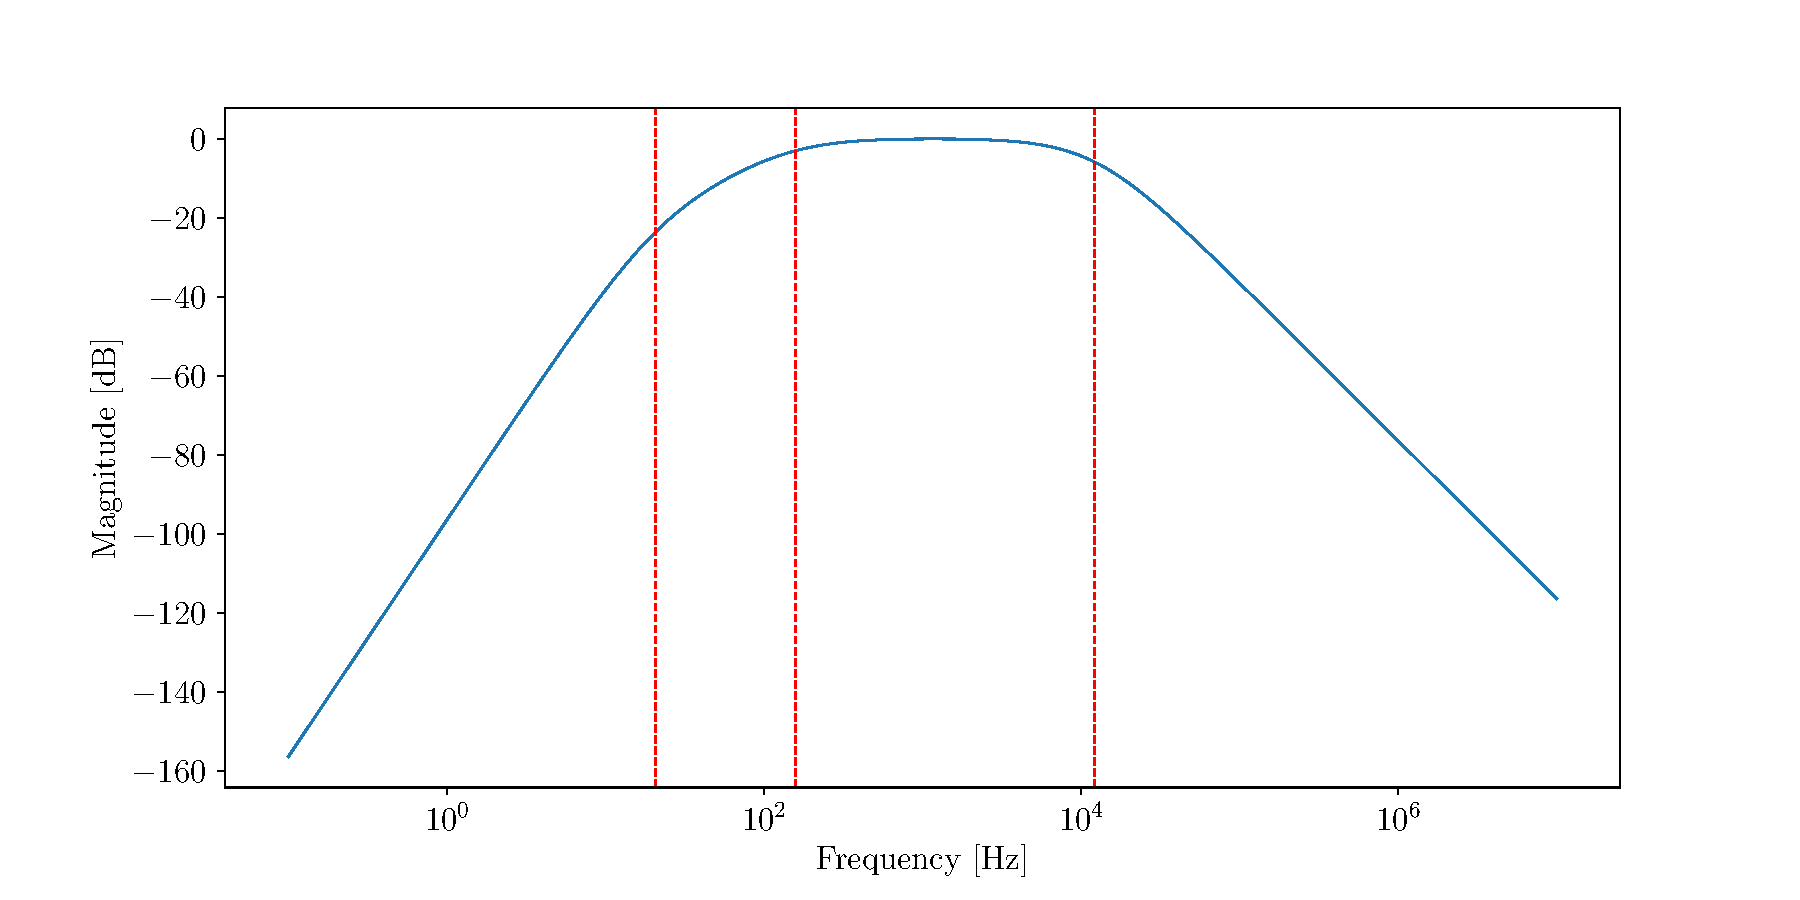
\includegraphics[height=5cm]{../figs/signal_filtering/bode_mag.pdf}};
\end{tikzpicture}
}
\end{frame}

%---------------------------------------------------------------%

\stepcounter{sectionframecount}
\begin{frame}[t]{Filter Application at Ground: ODE Approach}
\vspace{-10pt}
Common filtering techniques not suitable for our unstructured grid.

\uncover<2->
{
\vspace{8pt}
Convert transfer function in complex frequency domain:

\begin{equation}
  \tilde{P}(\chi) =P(\chi)\dfrac{K \chi^3}{(\chi+a)^2(\chi+b)(\chi+c)^2},
\end{equation}

to a \textbf{system of ODE's} in the $\tau$ domain (to solve in \textit{ground} boundary):
}

\uncover<3->
{
\begin{equation}
  \dfrac{d\bar{u}}{d\tau} =
      \begin{pmatrix}
          0 & 1 & 0 & 0 & 0\\
          -a^2 & -2a & 0 & 0 & 0\\
          0 & 0 & 0 & 1 & 0\\
          -K^{1/3}a^2 & -2K^{1/3}a & -c^2 & -2c & 0\\
          0 & 0 & 0 &K^{1/3} & -b
      \end{pmatrix}
      \bar{u}
      +
      \begin{pmatrix}
          0 \\
          K^{1/3}p(\tau)\\
          0\\
          K^{2/3}p(\tau)\\
          0
      \end{pmatrix},
  \end{equation}
where $\bar{u}=(u_0,u_1,u_2,u_3,\tilde{p})^T$, with homogeneous initial conditions.
}
\end{frame}

%=============================================================================%
%=============================================================================%
%=============================================================================%
% Section: Output Error Estimation

\begin{frame}[plain, t]
  \vspace{2cm}
  \centering
  {\usebeamerfont{title}\usebeamercolor[fg]{title}Output Error Estimation}

  \begin{tikzpicture}[remember picture,overlay]
    % Place the full image (faded version)
    \node[anchor=north east, xshift=-0.6cm, yshift=-3.5cm, opacity=0.2] (img)
      at (current page.north east) {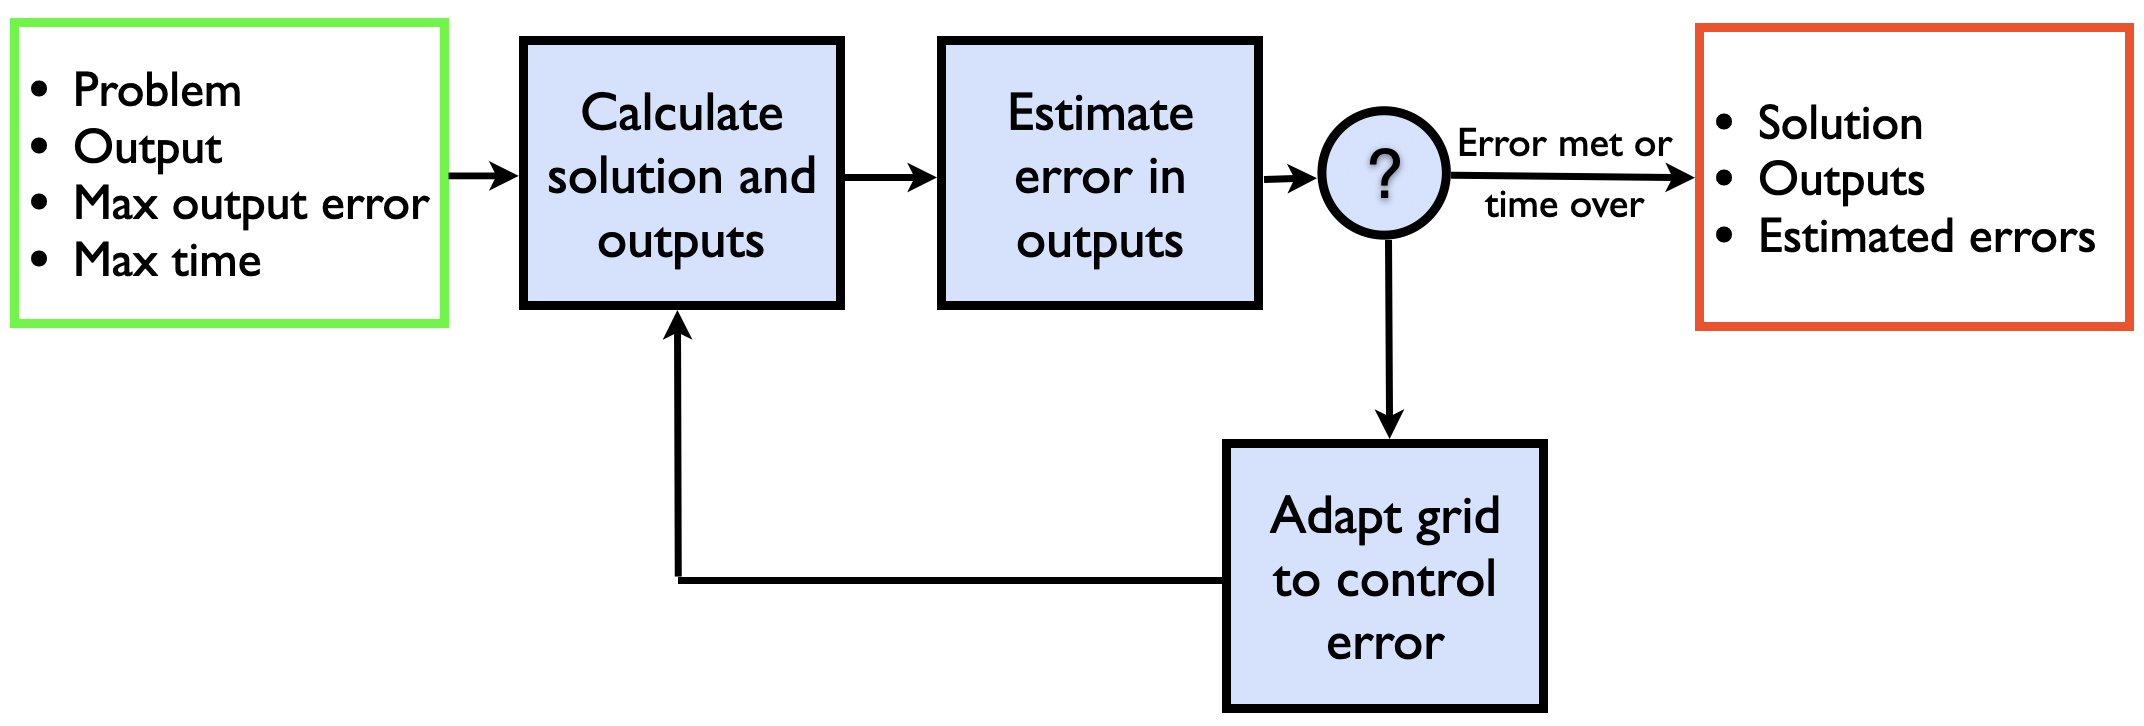
\includegraphics[height=3.8cm]{../figs/mesh_adaptation/adaptation_cycle.png}};

    % Define coordinates for the region to emphasize relative to the image node.
    % These coordinates are offsets from the image's north west corner.
    \coordinate (clipA) at ($(img.north west)+(5cm,-0.29cm)$);
    \coordinate (clipB) at ($(img.north west)+(6.8cm,-1.8cm)$);

    % Overlay a copy of the image clipped to the region of interest (full opacity).
    \begin{scope}[remember picture,overlay]
      \clip (clipA) rectangle (clipB);
      \node[anchor=north east, xshift=-0.6cm, yshift=-3.5cm]
        at (current page.north east) {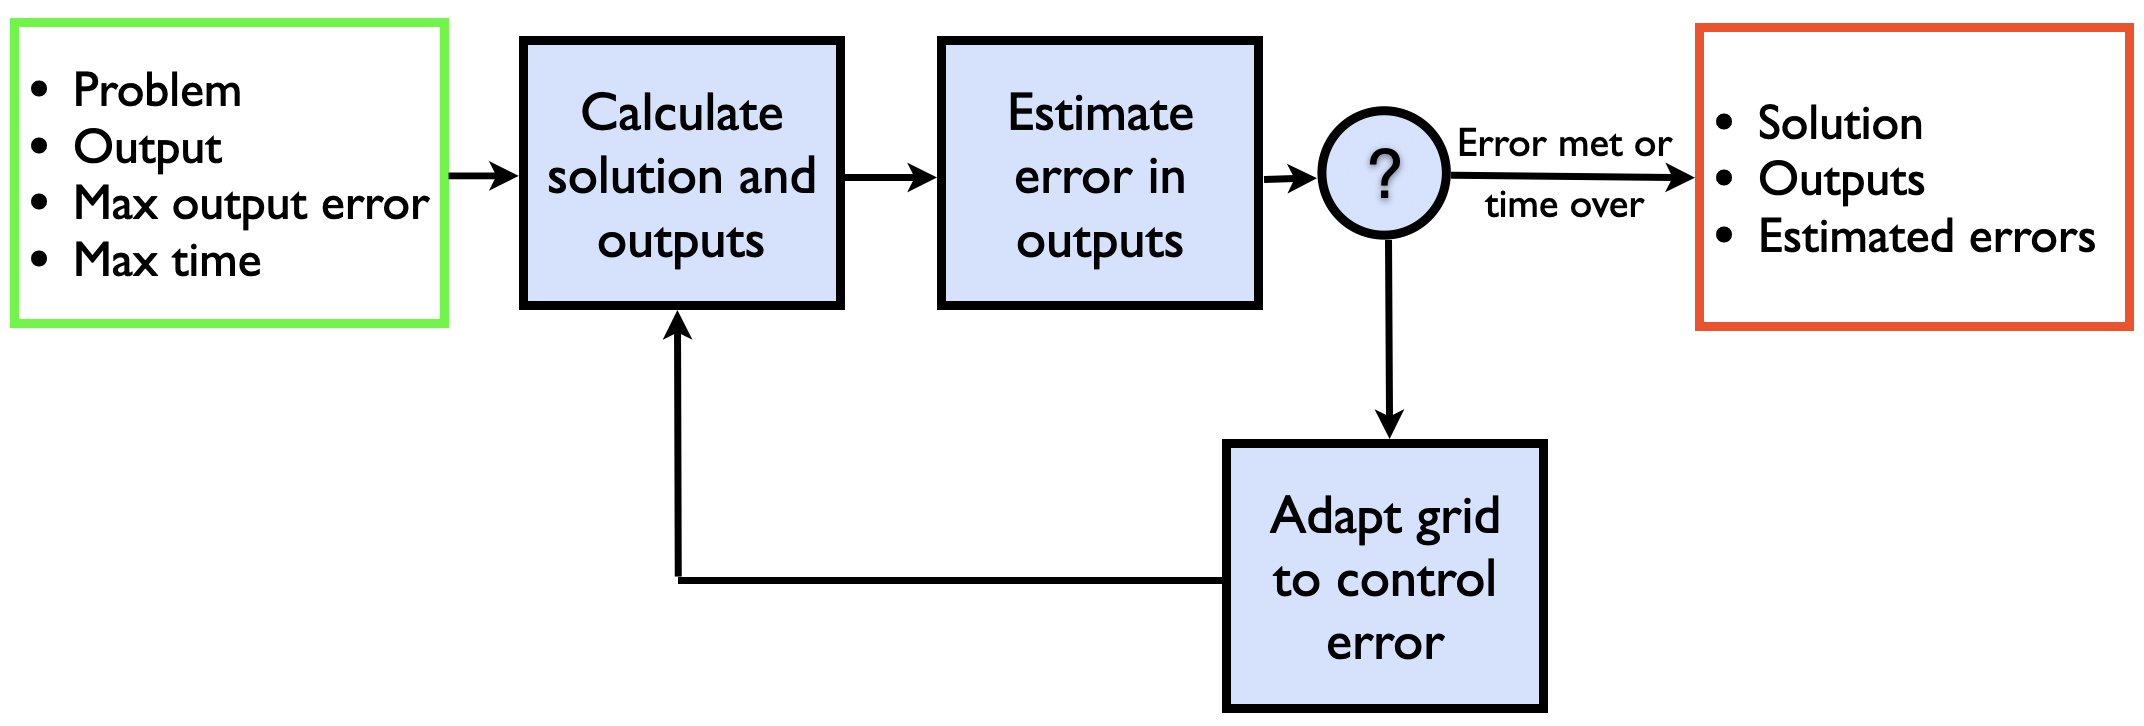
\includegraphics[height=3.8cm]{../figs/mesh_adaptation/adaptation_cycle.png}};
    \end{scope}

    % Draw a red dashed box around the highlighted region.
    \draw[red, dashed, thick] (clipA) rectangle (clipB);
  \end{tikzpicture}

\end{frame}

\section{Output Error Estimation}

\setsectionframes{5}

\stepcounter{sectionframecount}
\begin{frame}[t]{Output Functional and Error}
  We consider the following output functional:
  \begin{equation}
    \mathcal{J}(\boldsymbol{u}) := \int_{\text{ground}} [\tilde{p}(\tau)]^2~d\tau.
    \label{e:output_functional}
  \end{equation}

\uncover<2->
{
\vspace{10pt}
We define output error as:

\begin{equation}
  \varepsilon (\boldsymbol{u}_h) := \mathcal{J}(\boldsymbol{u}) - \mathcal{J}(\boldsymbol{u}_h).
\end{equation}

\vspace{8pt}
For our nonlinear problem, the output error can be approximated using the \textbf{dual weighted residual} (DWR) method.
}

\uncover<3->
{
\vspace{10pt}
Needs \textbf{correction}\footnotemark for artificial viscosity term (asymptotically consistent).
}
\footnotetext{B. Couchman 2020}
\end{frame}

%---------------------------------------------------------------%

\stepcounter{sectionframecount}
\begin{frame}[t]{Residual Consistency}
\vspace{-10pt}
  \begin{itemize}
    \item We say a form $\mathcal{R}^C$ is \textbf{consistent} if:
    \begin{equation}
      \mathcal{R}^C(\boldsymbol{v},\boldsymbol{u}) = 0,~~\forall \boldsymbol{v} \in \mathcal{V},
    \end{equation}
    where $\boldsymbol{u}$ is the exact solution.

    \uncover<2->
    {
    \item We say a form $\mathcal{R}^A$ is \textbf{asymptotically consistent} if:

    \begin{equation}
      \mathcal{R}^A(\boldsymbol{v},\boldsymbol{u}) = \mathcal{O}(h^\alpha),~~\forall \boldsymbol{v} \in \mathcal{V},
      \label{e:asymptotic_consistent}
    \end{equation}
    where $\boldsymbol{u}$ is the exact solution, $\alpha>0$, and $h$ is a characteristic element size in $\mathcal{T}_h$.
    }
  \end{itemize}

\uncover<3->
{
\vspace{10pt}
In our situation:
\vspace{-5pt}
\begin{equation}
  \begin{split}
  \mathcal{R}(\boldsymbol{v}_h,&\boldsymbol{u}_h) :=
  \underbrace{\mathcal{R}^C(\boldsymbol{v}_h,\boldsymbol{u}_h)}_{:= \mathcal{R}^{CG}} + \underbrace{\mathcal{R}^A(\boldsymbol{v}_h,\boldsymbol{u}_h)}_{:=\mathcal{R}^{\text{AV}}}.
  \end{split}
  \label{e:residual_C_A_decomposition}
\end{equation}
}
\end{frame}

%---------------------------------------------------------------%

\stepcounter{sectionframecount}
\begin{frame}[t]{Dual Problem and Error for Linear Case}
  \vspace{-10pt}
  We assume linear residual and output functional, and define the \textbf{dual} (adjoint) problem as:

  \vspace{5pt}
  Find $\boldsymbol{\psi} \in \mathcal{W}$ such that:

  \begin{equation}
      \mathcal{R}(\boldsymbol{\psi},\boldsymbol{w}) - \mathcal{J}(\boldsymbol{w}) = 0, ~~\forall \boldsymbol{w} \in \mathcal{W}.
  \end{equation}

  \uncover<2->
  {
  From there:
  }
  \vspace{2pt}
  \begin{equation}
    \begin{split}
      \uncover<2->{\varepsilon(\boldsymbol{u}_h) &= \mathcal{J}(\boldsymbol{u}) - \mathcal{J}(\boldsymbol{u}_h)~~~(\Delta \boldsymbol{u}:= \boldsymbol{u}-\boldsymbol{u}_h)} \\
      &\uncover<2->{= \mathcal{J}(\Delta \boldsymbol{u})} \\
      &\uncover<3->{= \mathcal{R}(\boldsymbol{\psi},\Delta \boldsymbol{u})} \\
      &\uncover<4->{= \underbrace{\mathcal{R}^C(\boldsymbol{\psi},\boldsymbol{u})}_{= 0} + \mathcal{R}^A(\boldsymbol{\psi},\boldsymbol{u}) \underbrace{- \mathcal{R}^C(\boldsymbol{\psi},\boldsymbol{u}_h) - \mathcal{R}^A(\boldsymbol{\psi},\boldsymbol{u}_h)}_{=-\mathcal{R}(\boldsymbol{\psi},\boldsymbol{u}_h)}} \\
      &\uncover<5->{= -\Big[\mathcal{R}(\boldsymbol{\psi},\boldsymbol{u}_h) - \mathcal{R}^A(\boldsymbol{\psi},\boldsymbol{u})\Big]\text{ (Dual weighted residual error expression)}}
    \end{split}
  \end{equation}
\end{frame}

%---------------------------------------------------------------%

\stepcounter{sectionframecount}
\begin{frame}[t]{Approximations: DWR Error Estimate}
  So far:
  \begin{equation}
    \varepsilon(\boldsymbol{u}_h) = -\Big[\mathcal{R}(\boldsymbol{\psi},\boldsymbol{u}_h) - \mathcal{R}^A(\boldsymbol{\psi},\boldsymbol{u})\Big].
  \end{equation}

  \uncover<2->
  {
  \textbf{Issues:}

  \begin{itemize}
    \item Primal exact solution $\boldsymbol{u}$ is not available.
    \item Residual and output functional are in general nonlinear.
    \item Even if they are linear, adjoint exact solution $\boldsymbol{\psi}$ is not available.
  \end{itemize}
  }

  \uncover<3->
  {
  \vspace{10pt}
  \textbf{First approximation}:

  \begin{equation}
    \mathcal{R}^A(\boldsymbol{\psi},\boldsymbol{u}) \approx
    \mathcal{R}^A(\boldsymbol{\psi},\boldsymbol{u}_h),
  \end{equation}
  justified on a shock dominated problem with AV.
  }
\end{frame}

%---------------------------------------------------------------%

\stepcounter{sectionframecount}
\begin{frame}[t]{Approximations: DWR Error Estimate}
  \vspace{-5pt}
  \textbf{Second approximation:}

  \vspace{10pt}
  $\boldsymbol{\psi}$ is approximated with a numerical adjoint $\boldsymbol{\psi}_{\hat{h}}$ defined by\footnotemark:

  \uncover<2->
  {
  $\boldsymbol{\psi}_{\hat{h}} \in \mathcal{V}_{\hat{h},\hat{p}}$ such that:

  \begin{equation}
    \mathcal{R}^\prime[\boldsymbol{u}_h](\boldsymbol{\psi}_{\hat{h}},\tilde{\boldsymbol{u}}) - \mathcal{J}^\prime[\boldsymbol{u}_h](\tilde{\boldsymbol{u}}) = 0,~~~\forall \tilde{\boldsymbol{u}} \in \mathcal{V}_{\hat{h},\hat{p}},
  \end{equation}
  where:

  \begin{itemize}
    \item $\mathcal{R}^\prime[\boldsymbol{u}_h]$ and $\mathcal{J}^\prime[\boldsymbol{u}_h]$ are the linearizations of $\mathcal{R}$ and $\mathcal{J}$ about $\boldsymbol{u}_h$.
    \item $\tilde{\boldsymbol{u}}$ represents a perturbation from $\boldsymbol{u}_h$.
    \item The space $\mathcal{V}_{\hat{h},\hat{p}}$ contains polynomials of order $\hat{p}=p+1$.
  \end{itemize}
  }

  \uncover<3->
  {
  \vspace{10pt}
  \textbf{Final DWR error estimate:}
  \begin{equation}
    \varepsilon(\boldsymbol{u}_h) \approx -\Big[\mathcal{R}(\boldsymbol{\psi}_{\hat{h}},\boldsymbol{u}_h) - \mathcal{R}^A(\boldsymbol{\psi}_{\hat{h}},\boldsymbol{u}_h)\Big].
  \end{equation}
  }
\footnotetext{M. Yano and D. L. Darmofal 2012}

\end{frame}

%=============================================================================%
%=============================================================================%
%=============================================================================%
% Section: Mesh adaptation

\begin{frame}[plain, t]
  \vspace{2cm}
  \centering
  {\usebeamerfont{title}\usebeamercolor[fg]{title}Mesh Adaptation}

  \begin{tikzpicture}[remember picture,overlay]
    % Place the full image (faded version)
    \node[anchor=north east, xshift=-0.6cm, yshift=-3.5cm, opacity=0.2] (img)
      at (current page.north east) {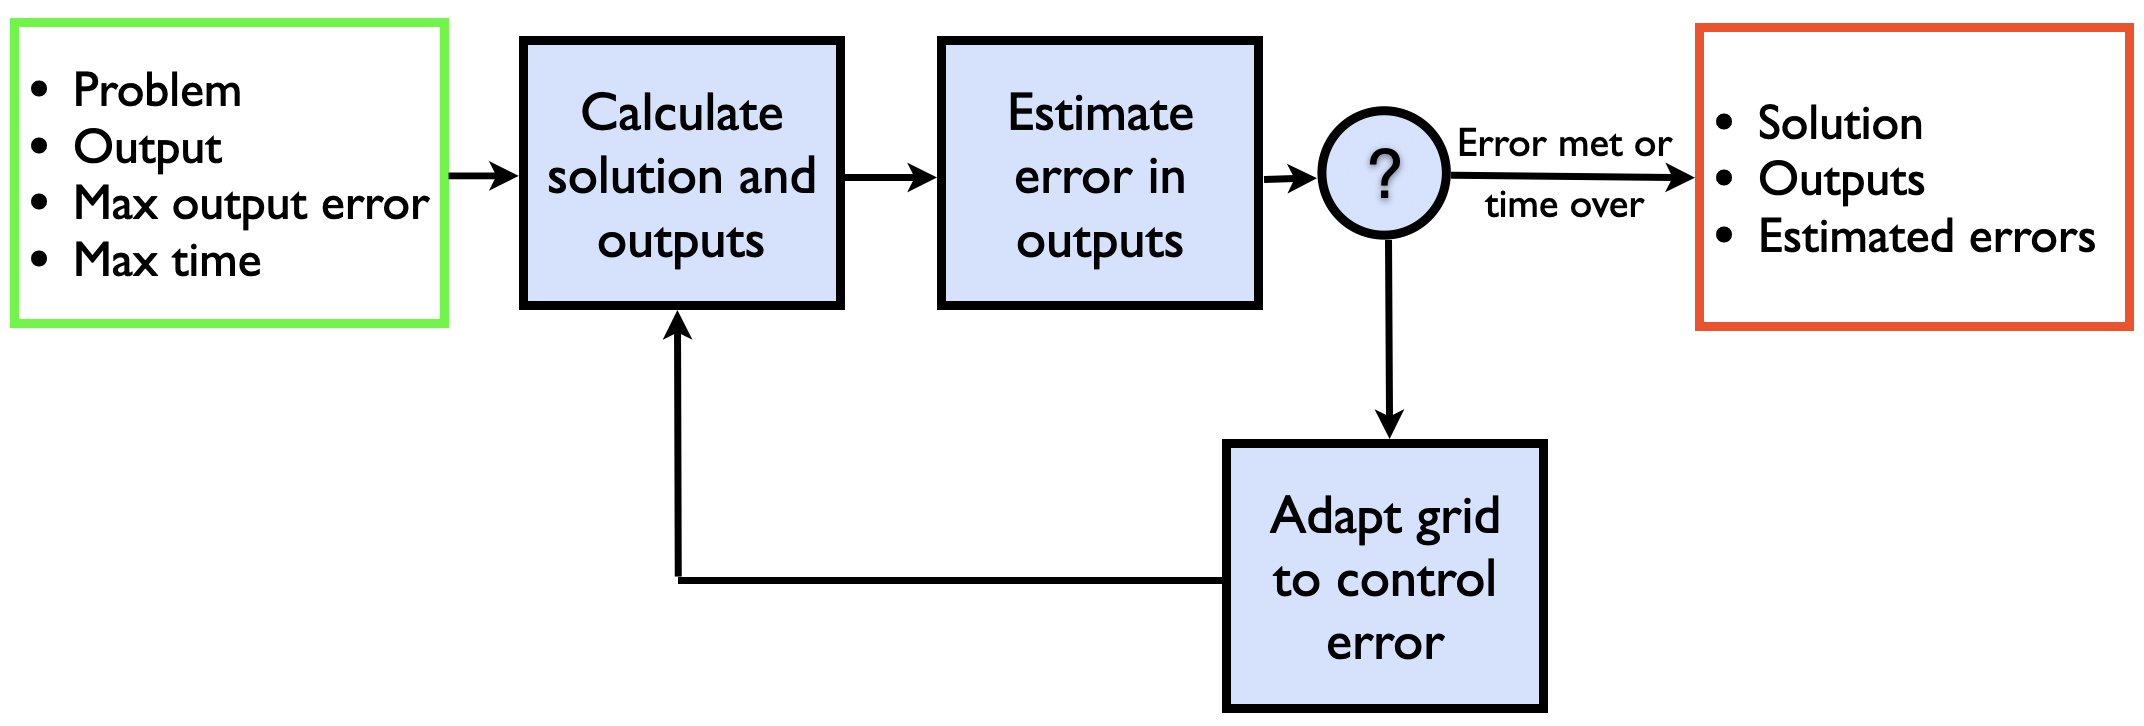
\includegraphics[height=3.8cm]{../figs/mesh_adaptation/adaptation_cycle.png}};

    % Define coordinates for the region to emphasize relative to the image node.
    % These coordinates are offsets from the image's north west corner.
    \coordinate (clipA) at ($(img.north west)+(6.45cm,-2.4cm)$);
    \coordinate (clipB) at ($(img.north west)+(8.3cm,-3.95cm)$);

    % Overlay a copy of the image clipped to the region of interest (full opacity).
    \begin{scope}[remember picture,overlay]
      \clip (clipA) rectangle (clipB);
      \node[anchor=north east, xshift=-0.6cm, yshift=-3.5cm]
        at (current page.north east) {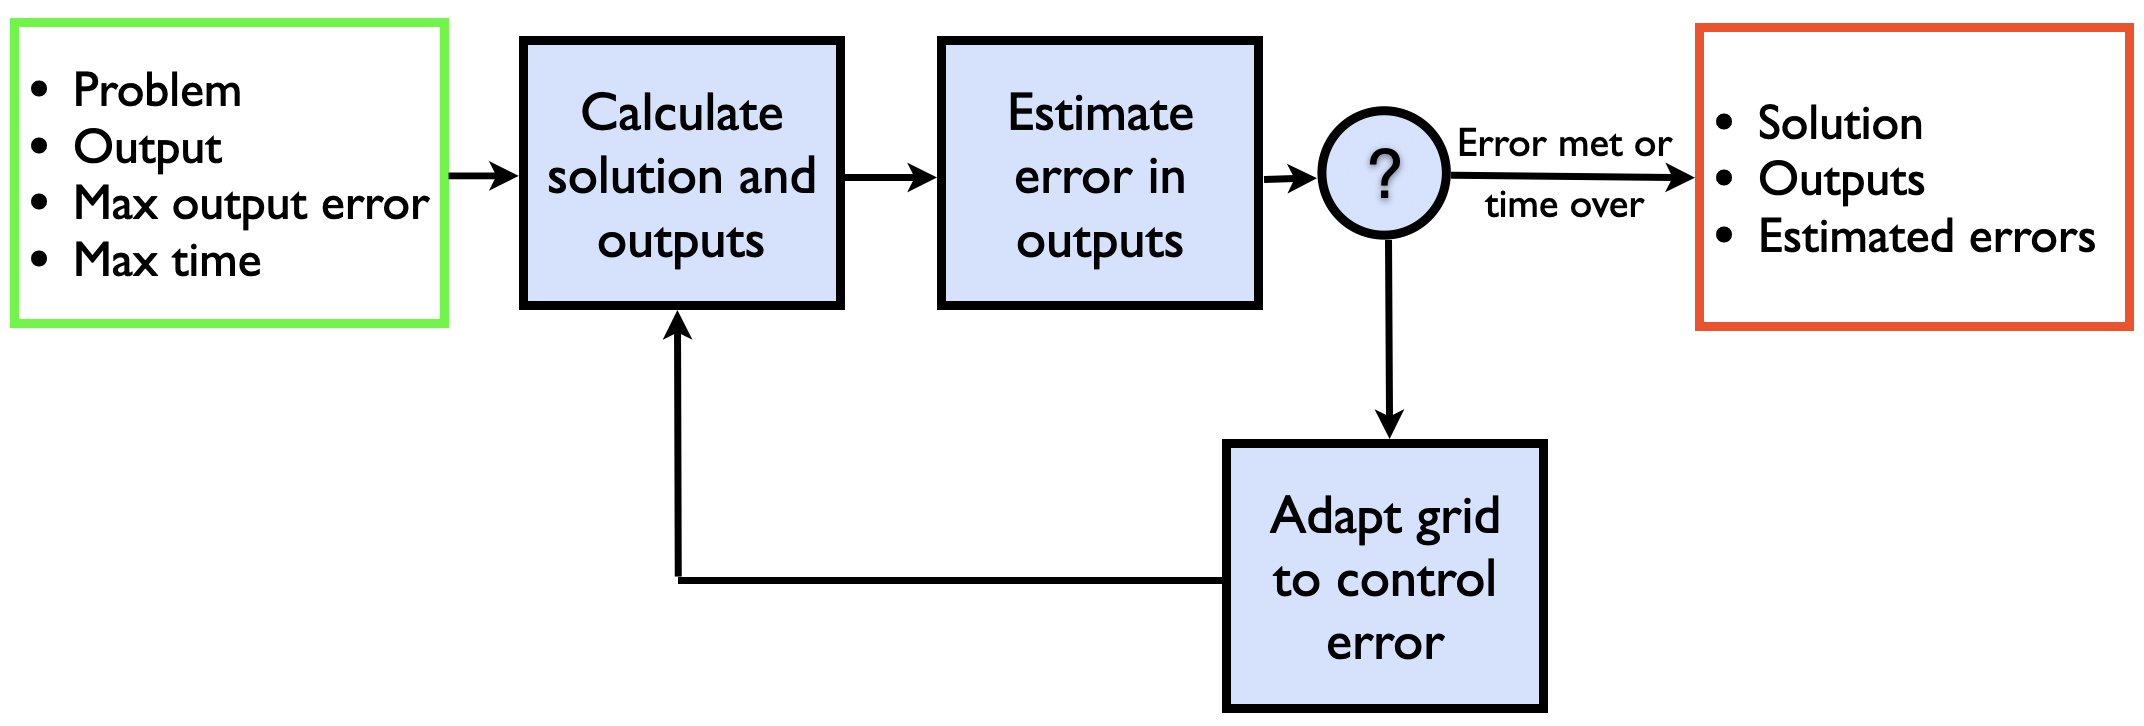
\includegraphics[height=3.8cm]{../figs/mesh_adaptation/adaptation_cycle.png}};
    \end{scope}

    % Draw a red dashed box around the highlighted region.
    \draw[red, dashed, thick] (clipA) rectangle (clipB);
  \end{tikzpicture}

\end{frame}

\section{Mesh Adaptation}

\setsectionframes{3}

\stepcounter{sectionframecount}

%---------------------------------------------------------------%

\begin{frame}[t]{Continuous Optimization: Mesh-Metric Duality}
\vspace{-10pt}
Want mesh producing the smallest output error indicator $\mathcal{E}$:

\begin{equation}
  \hat{\mathcal{T}}_h = \arg \inf_{\mathcal{T}_h \in \mathbb{T}(\Omega)} \mathcal{E}(\mathcal{T}_h),~~~\mathcal{C}(\mathcal{T}_h) < C.
\end{equation}

\uncover<2->
{
\textbf{Continuous relaxation}\footnotemark to address intractability of discrete problem.

\begin{equation}
  \hat{\mathcal{M}} = \arg\inf_{\mathcal{M} \in \mathbb{M}(\Omega)} \mathcal{E}(\mathcal{M}),~~~\mathcal{C}(\mathcal{M}) < C
\end{equation}

\begin{tikzpicture}[remember picture,overlay]
  \node[anchor=north east, xshift=-1.1cm, yshift=-5.1cm]
  at (current page.north east) {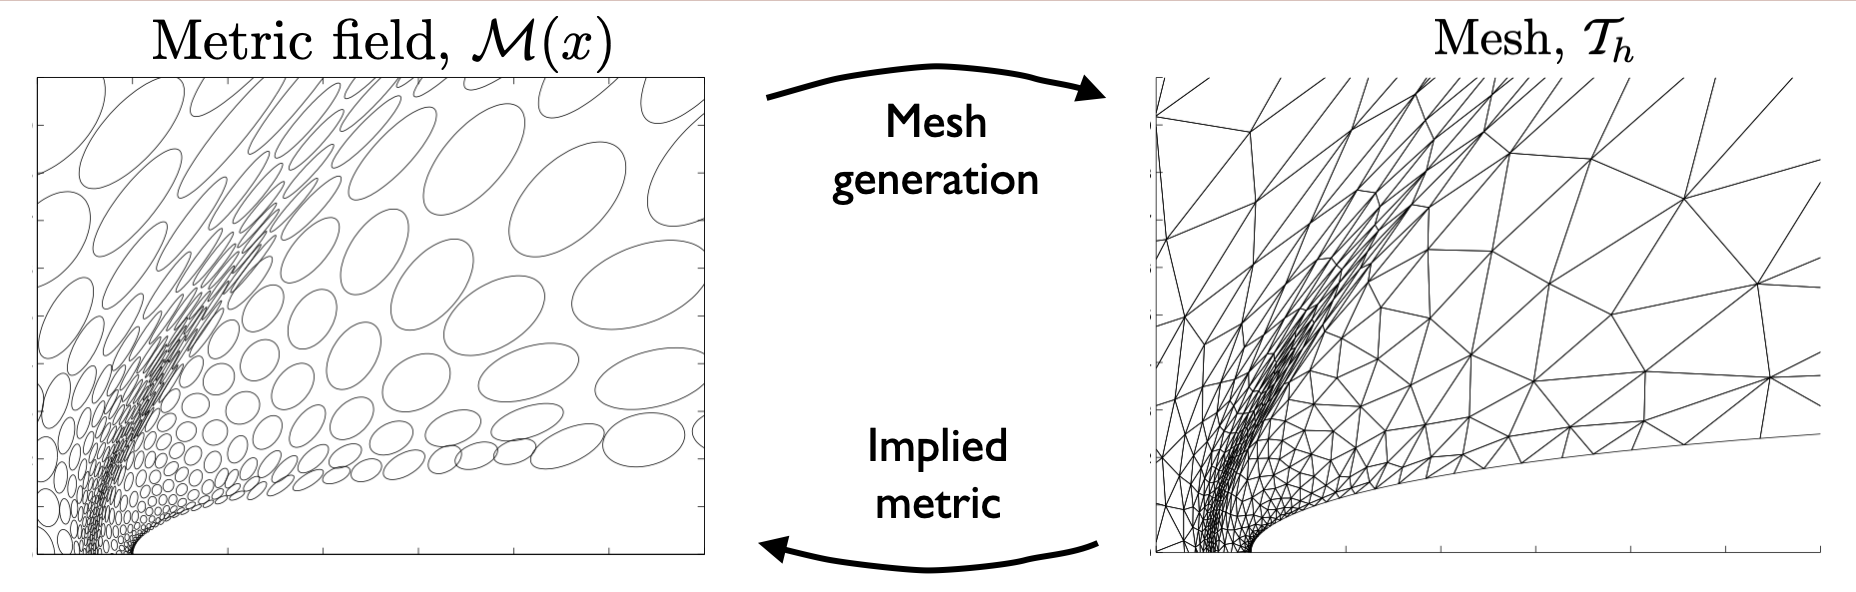
\includegraphics[height=3.4cm]{../figs/mesh_adaptation/mesh_metric_duality.png}};
\end{tikzpicture}
}
\footnotetext{A. Loseille and F. Alauzet 2011}

\end{frame}

%---------------------------------------------------------------%

\stepcounter{sectionframecount}
\begin{frame}[t]{MOESS\footnote{M. Yano and D. L. Darmofal 2012}: Error Sampling and Synthesis}
\vspace{-5pt}
\textbf{Need model for error indicator $\mathcal{E}(\mathcal{M})$}: How $\mathcal{E}$ changes with $\mathcal{M}$.

\uncover<2->
{
\vspace{10pt}
\textbf{First step:} Compute nodal\footnote{T. Richter and T. Wick 2015} error indicators based on the DWR error estimate. Use partition of unity given by linear tent functions $\{\phi_v\}$.
}

\uncover<3->
{
\begin{equation}
  \varepsilon_v := -\mathcal{R}(\phi_v \Delta \boldsymbol{\psi}_{\hat{h}},\boldsymbol{u}_h) + \mathcal{R}^A(\phi_v\boldsymbol{\psi}_{\hat{h}},\boldsymbol{u}_h),
  \label{e:corrected_dwr_nodal}
\end{equation}

\begin{equation}
  \eta_v := |\mathcal{R}(\phi_v \Delta \boldsymbol{\psi}_{\hat{h}},\boldsymbol{u}_h)| + |\mathcal{R}^A(\phi_v\boldsymbol{\psi}_{\hat{h}},\boldsymbol{u}_h)|,~~~ \eta := \sum_{v} \eta_v \equiv \mathcal{E}
  \label{e:corrected_dwr_nodal}
\end{equation}
}

\uncover<4->
{
\textbf{Next:} Recompute solution and nodal indicators in refined \textit{local patches} in the mesh.

\vspace{5pt}
The comparison of the nodal error indicators before and after the local solves gives information about how $\mathcal{E}$ changes with $\mathcal{M}$.
}
\end{frame}

%---------------------------------------------------------------%

\stepcounter{sectionframecount}
\begin{frame}[t]{MOESS: Error Sampling and Synthesis}

\uncover<2->
{
\textbf{Local solve:} Solve for $\boldsymbol{u}_h^\epsilon \in \mathcal{V}_{h,p}^\epsilon$ s.t. $\mathcal{R}_{\text{local}}(\boldsymbol{v}_h^\epsilon,\boldsymbol{u}_h^\epsilon) = 0,~~~\forall \boldsymbol{v}_h^\epsilon \in \mathcal{V}_{h,p}^\epsilon$.
}

\begin{tikzpicture}[remember picture,overlay]
  \node[anchor=north east, xshift=-1.4cm, yshift=-2.4cm]
  at (current page.north east) {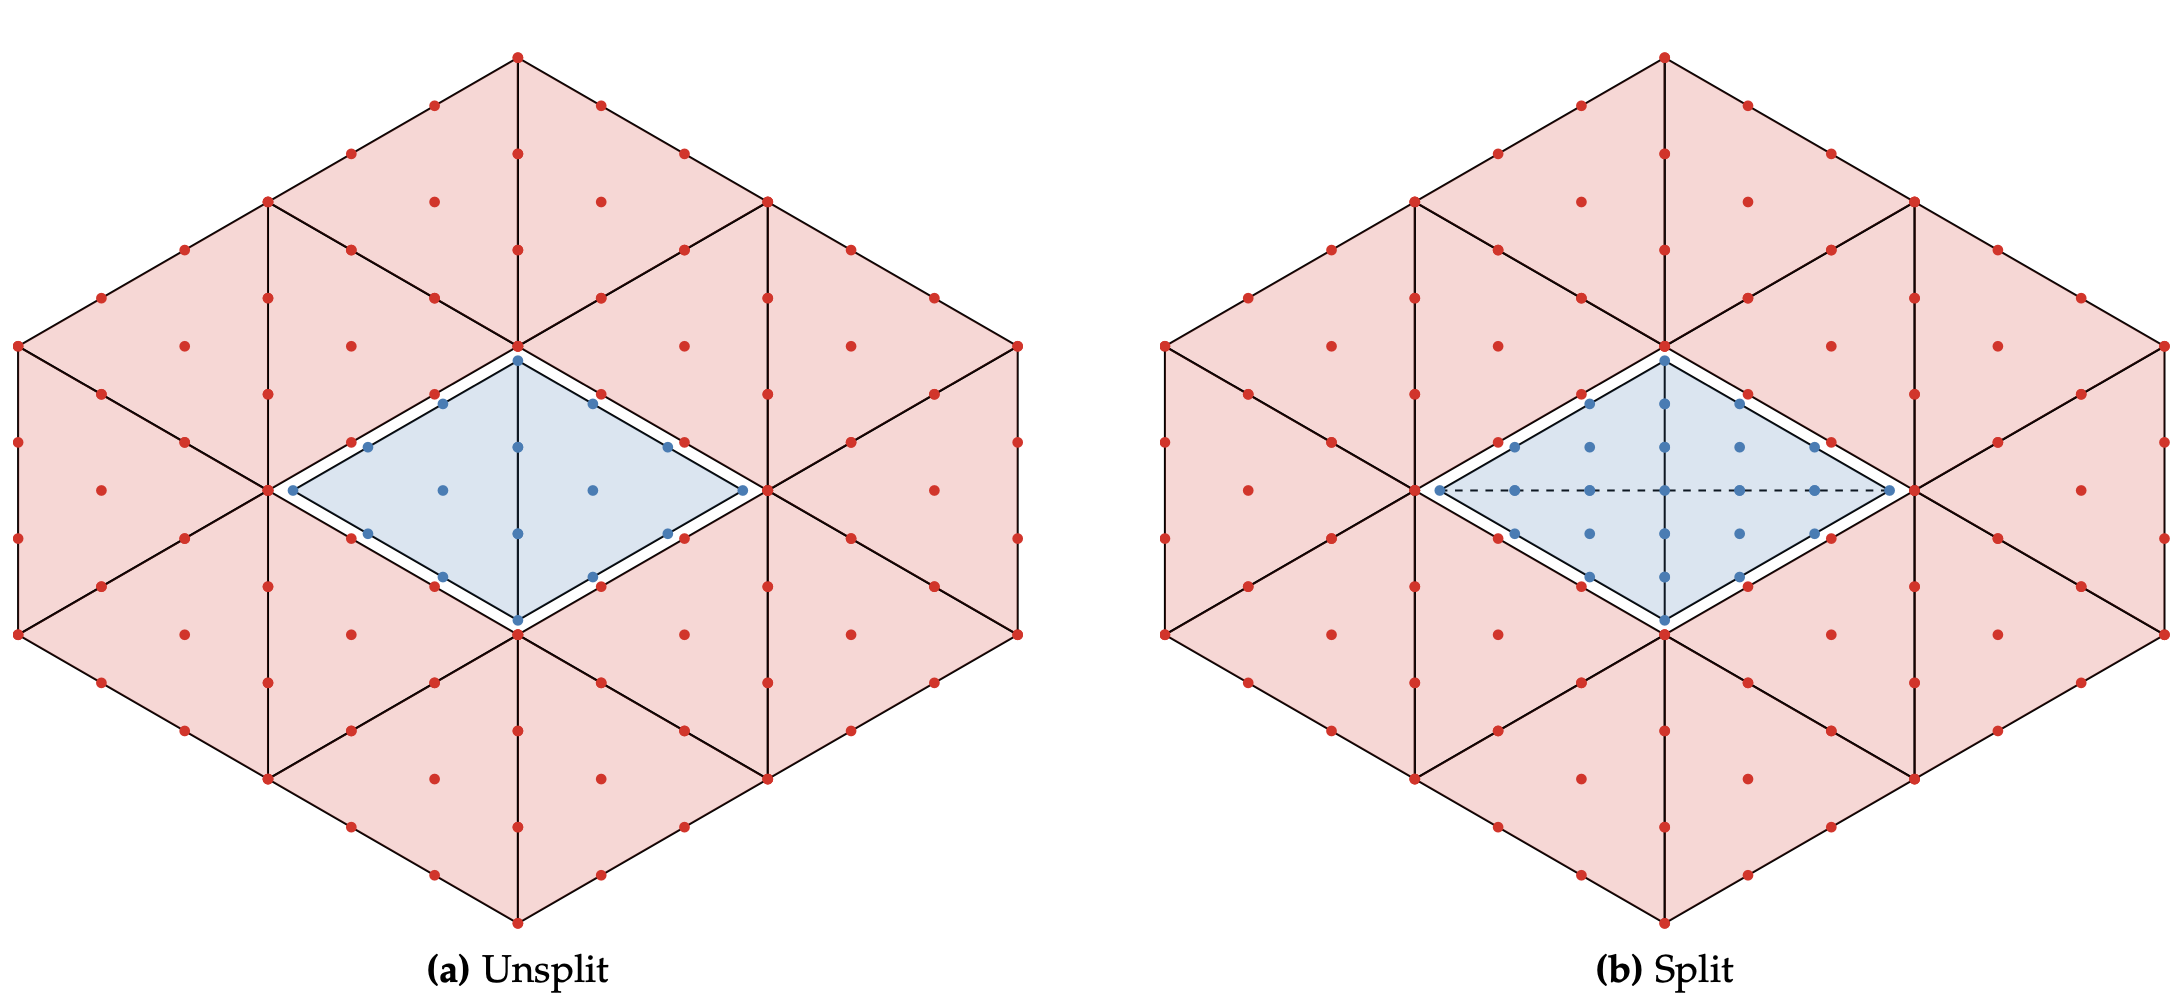
\includegraphics[height=4.5cm]{../figs/mesh_adaptation/local_patches.png}};
\end{tikzpicture}

\uncover<3->
{
\vspace{4.7cm}
\textbf{Nodal indicator for vertices in inner patch:}
\begin{equation}
  \eta_v^\epsilon = |\mathcal{R}_\text{local}(\phi_v \Delta \boldsymbol{\psi}_{\hat{h}},\boldsymbol{u}_h^\epsilon)| + |\mathcal{R}_\text{local}^A(\phi_v\boldsymbol{\psi}_{\hat{h}},\boldsymbol{u}^\epsilon_h)|.
  \label{e:dwr_ind_base_local}
\end{equation}
}
\end{frame}

%=============================================================================%
%=============================================================================%
%=============================================================================%
% Section: Results for Practial Case

\begin{frame}[plain, t]
  \vspace{2cm}
  \centering
  {\usebeamerfont{title}\usebeamercolor[fg]{title}Results for Practical Case}

  \begin{tikzpicture}[remember picture,overlay]
    % Place the full image (faded version)
    \node[anchor=north east, xshift=-0.6cm, yshift=-3.5cm, opacity=0.2] (img)
      at (current page.north east) {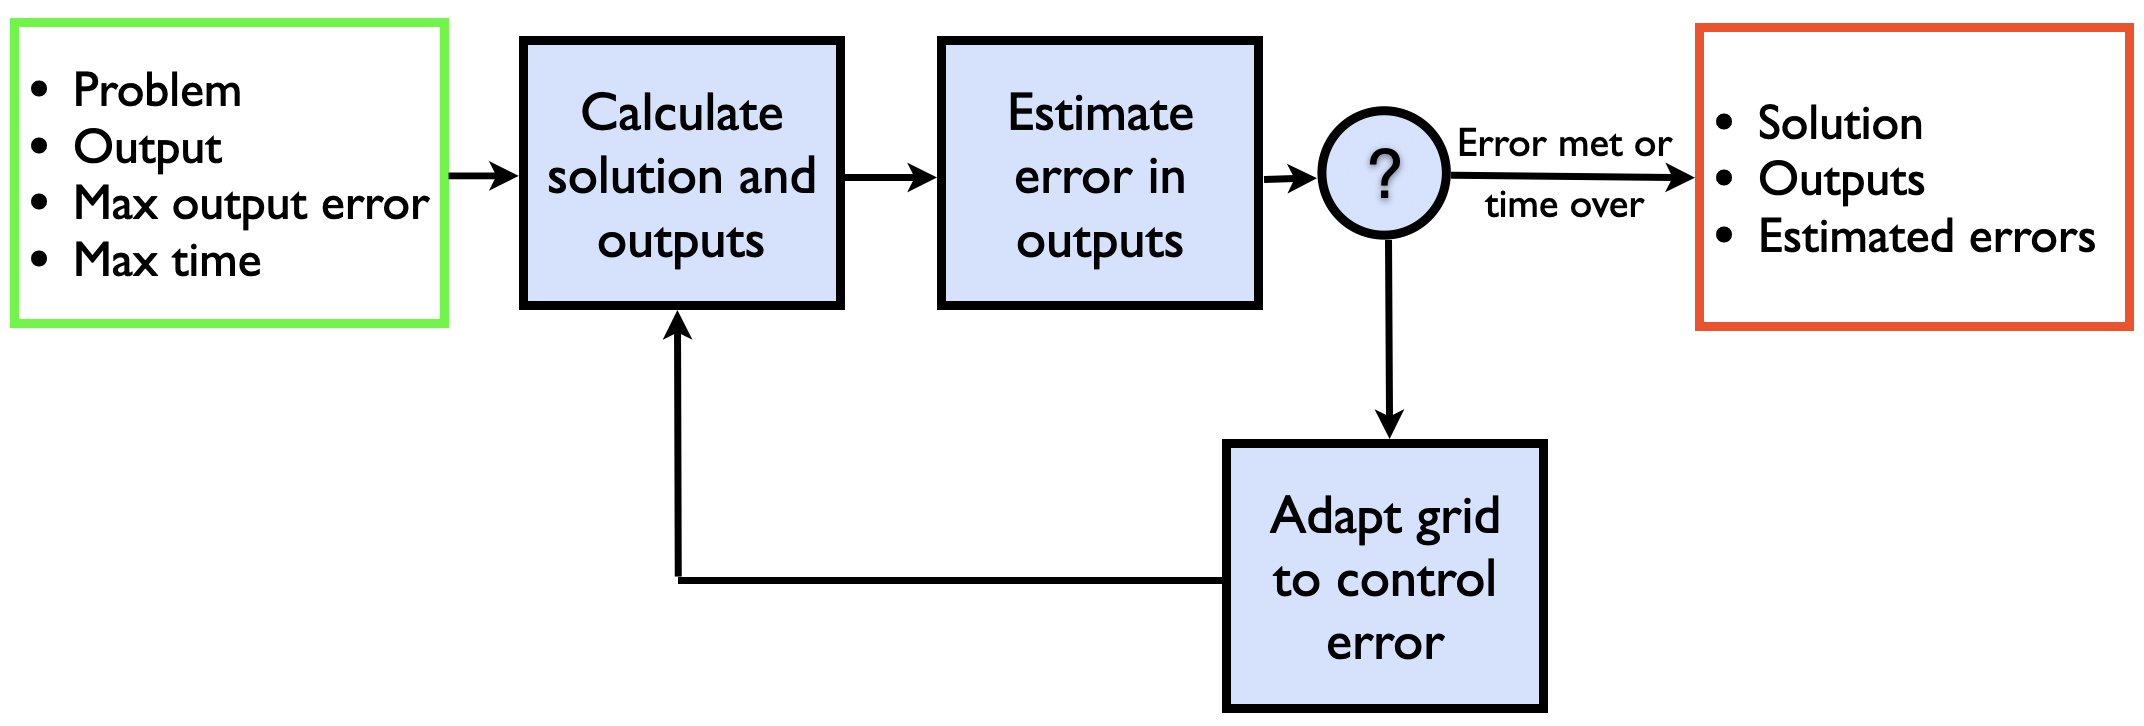
\includegraphics[height=3.8cm]{../figs/mesh_adaptation/adaptation_cycle.png}};

    % Define coordinates for the region to emphasize relative to the image node.
    % These coordinates are offsets from the image's north west corner.
    \coordinate (clipA) at ($(img.north west)+(0.1cm,-0.19cm)$);
    \coordinate (clipB) at ($(img.north west)+(2.55cm,-1.9cm)$);

    % Overlay a copy of the image clipped to the region of interest (full opacity).
    \begin{scope}[remember picture,overlay]
      \clip (clipA) rectangle (clipB);
      \node[anchor=north east, xshift=-0.6cm, yshift=-3.5cm]
        at (current page.north east) {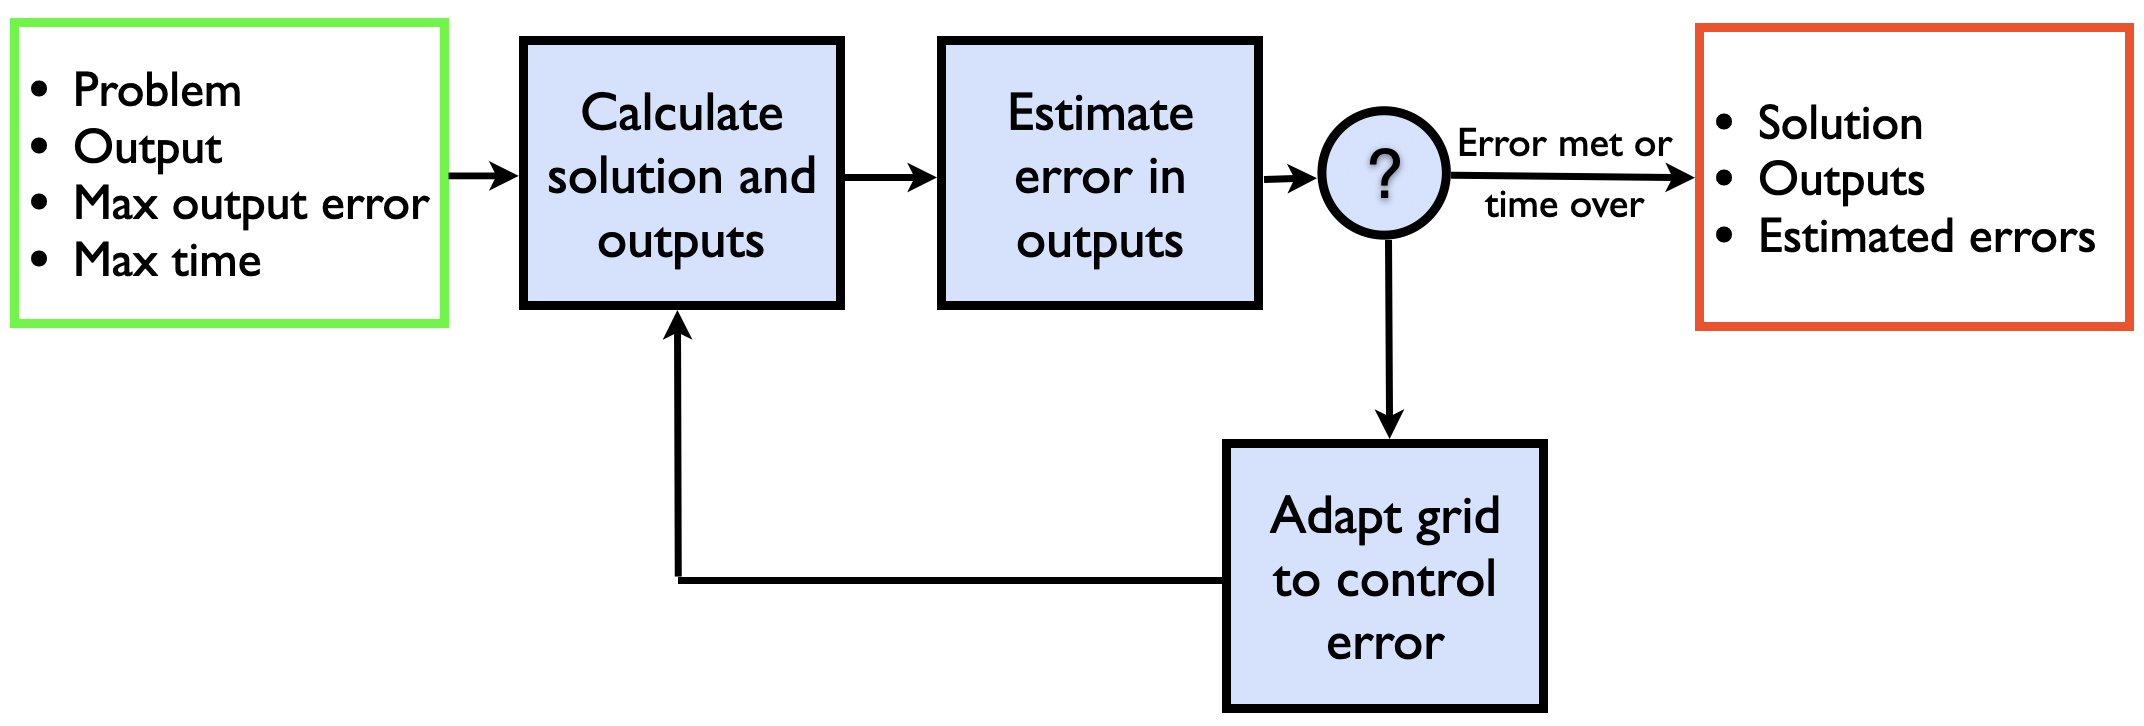
\includegraphics[height=3.8cm]{../figs/mesh_adaptation/adaptation_cycle.png}};
    \end{scope}

    % Draw a red dashed box around the highlighted region.
    \draw[red, dashed, thick] (clipA) rectangle (clipB);

    % Define coordinates for the region to emphasize relative to the image node.
    % These coordinates are offsets from the image's north west corner.
    \coordinate (clipAA) at ($(img.north west)+(8.95cm,-0.19cm)$);
    \coordinate (clipBB) at ($(img.north west)+(11.35cm,-1.95cm)$);

    % Overlay a copy of the image clipped to the region of interest (full opacity).
    \begin{scope}[remember picture,overlay]
      \clip (clipAA) rectangle (clipBB);
      \node[anchor=north east, xshift=-0.6cm, yshift=-3.5cm]
        at (current page.north east) {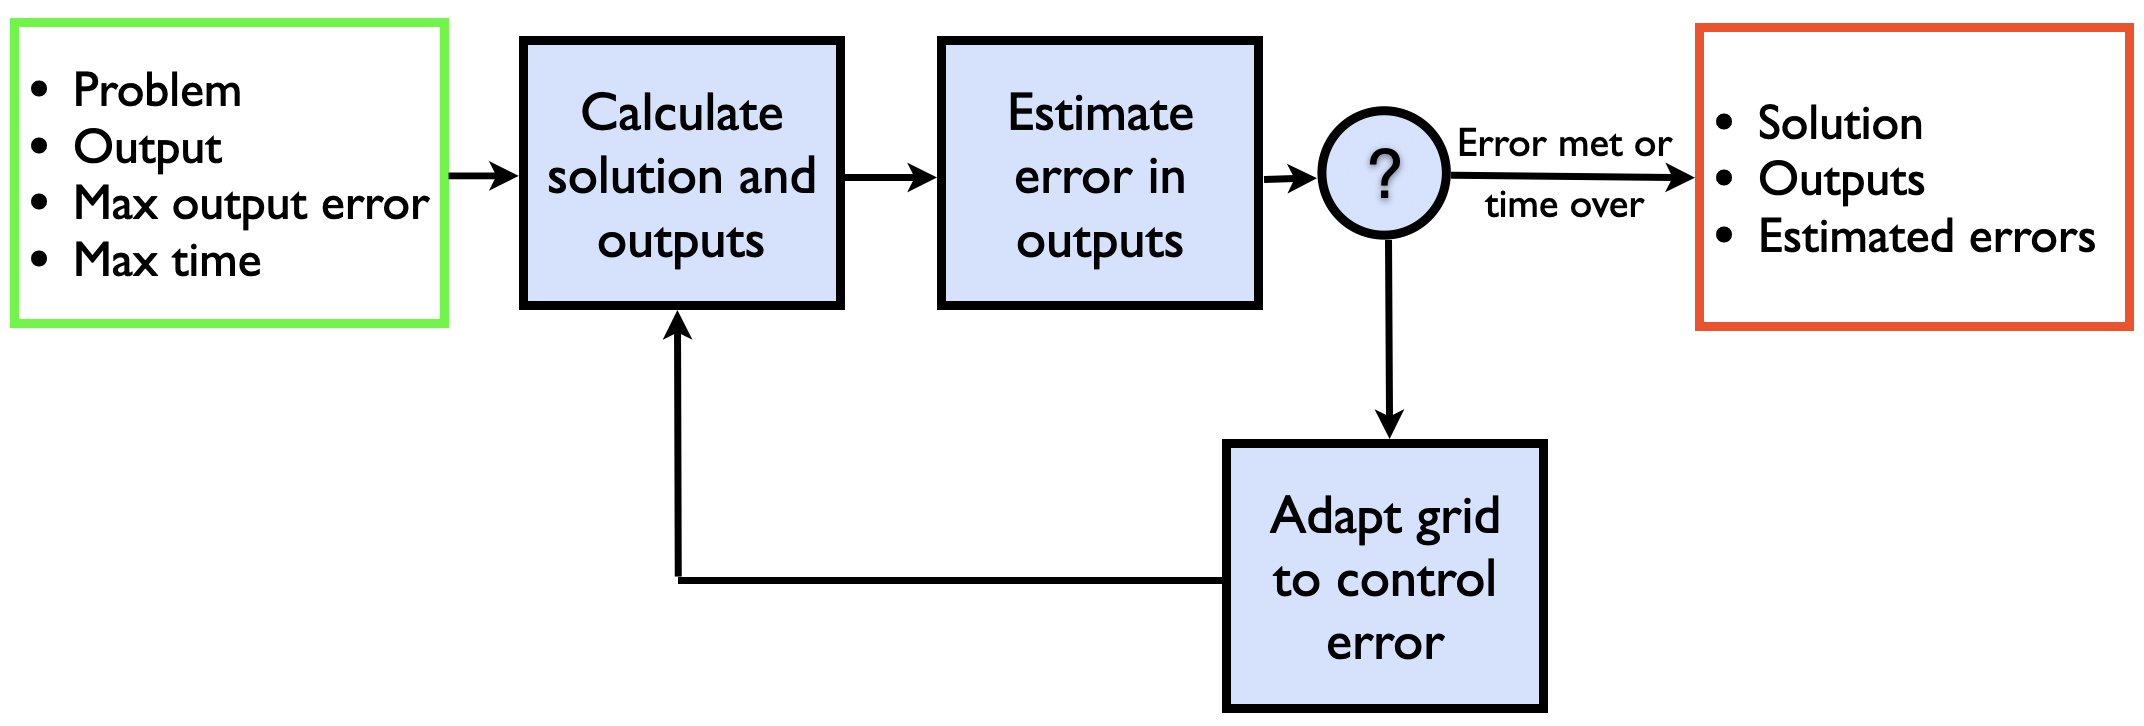
\includegraphics[height=3.8cm]{../figs/mesh_adaptation/adaptation_cycle.png}};
    \end{scope}

    % Draw a red dashed box around the highlighted region.
    \draw[red, dashed, thick] (clipAA) rectangle (clipBB);
  \end{tikzpicture}

\end{frame}

\section{Results for Practical Case}

\setsectionframes{8}

%---------------------------------------------------------------%

\stepcounter{sectionframecount}
\begin{frame}[t]{Preliminary: Implementation Notes}

\textbf{Software: Solution Adaptive Numerical Simulator (SANS)\footnotemark}
\begin{itemize}
  \item C++ framework to numerically solve partial differential equations.
  % \item Extensive use of templates for efficient yet general code.
  \item Supports several CG and DG discretizations, with output-based mesh adaptation.
  % \item Automatic differentiation via operator overloading.
  \item MPI parallelization.
  \item Unit testing and continuous integration.
  \item Open source.
\end{itemize}

\footnotetext{Galbraith et. al. 2015}

\end{frame}


%---------------------------------------------------------------%

\stepcounter{sectionframecount}
\begin{frame}[t]{Case Description}
\vspace{-14pt}
\begin{minipage}[t]{0.8\linewidth}
  \begin{itemize}
    \item Airplane Mach number: $M_a = 1.4$.
    \item Airplane altitude: $z_a = 16459.2$ m.
    \item Ground altitude: $110$ m.
    \uncover<2->
    {
    \item Nearfield signal (initial condition):
    }
  \end{itemize}
\end{minipage}

\uncover<2->
{
\begin{tikzpicture}[remember picture,overlay]
  \node[anchor=north east, xshift=-5.5cm, yshift=-4.3cm]
  at (current page.north east) {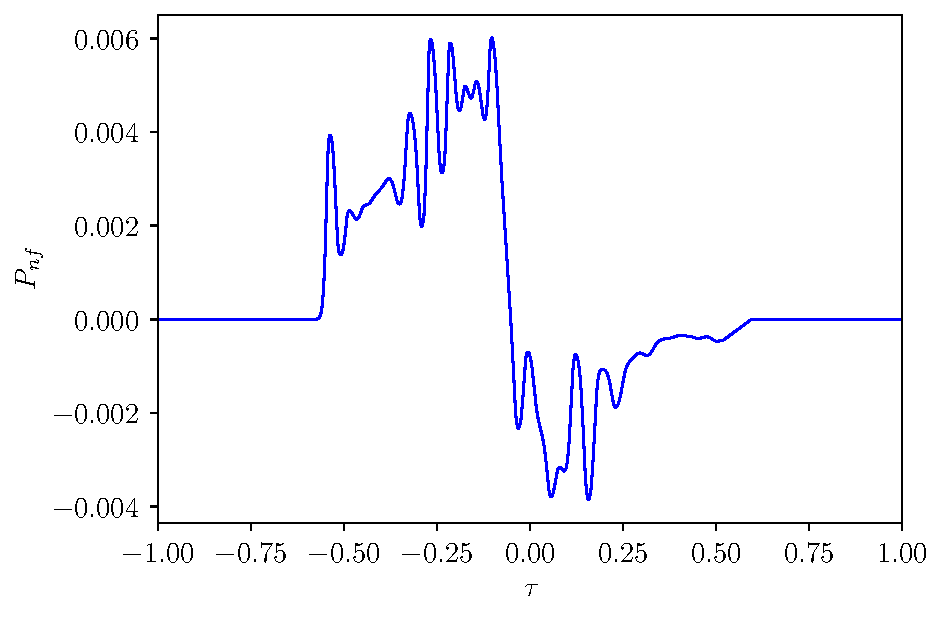
\includegraphics[height=4.4cm]{../figs/SBW3results/nearfield_nondimensional_SBW3_Case2_az0.pdf}};
\end{tikzpicture}
}
\begin{tikzpicture}[remember picture,overlay]

  \node[anchor=north east, xshift=0.7cm, yshift=-5.1cm] at (current page.north east) {%
    \begin{minipage}{0.5\textwidth}
      \begin{itemize}
        \uncover<3->
        {
        \item Domain dimensions:
        $\Omega = [-1,2] \times [0,257]$
        \vspace{8pt}
        \item Output for adaptation:
        $\mathcal{J}_{\text{BSEL}} = \int_{\text{ground}} [\tilde{p}(\tau)]^2~d\tau$
        }
        \uncover<4->
        {
        \vspace{8pt}
        \item Also for comparison:
        $\mathcal{J}_{p} = \int_{\text{ground}} [p(\tau)]^2~d\tau$
        }
      \end{itemize}
    \end{minipage}
  };
\end{tikzpicture}

\begin{tikzpicture}[remember picture,overlay]
  \node[anchor=north east, xshift=-0.2cm, yshift=-1.35cm]
    at (current page.north east) {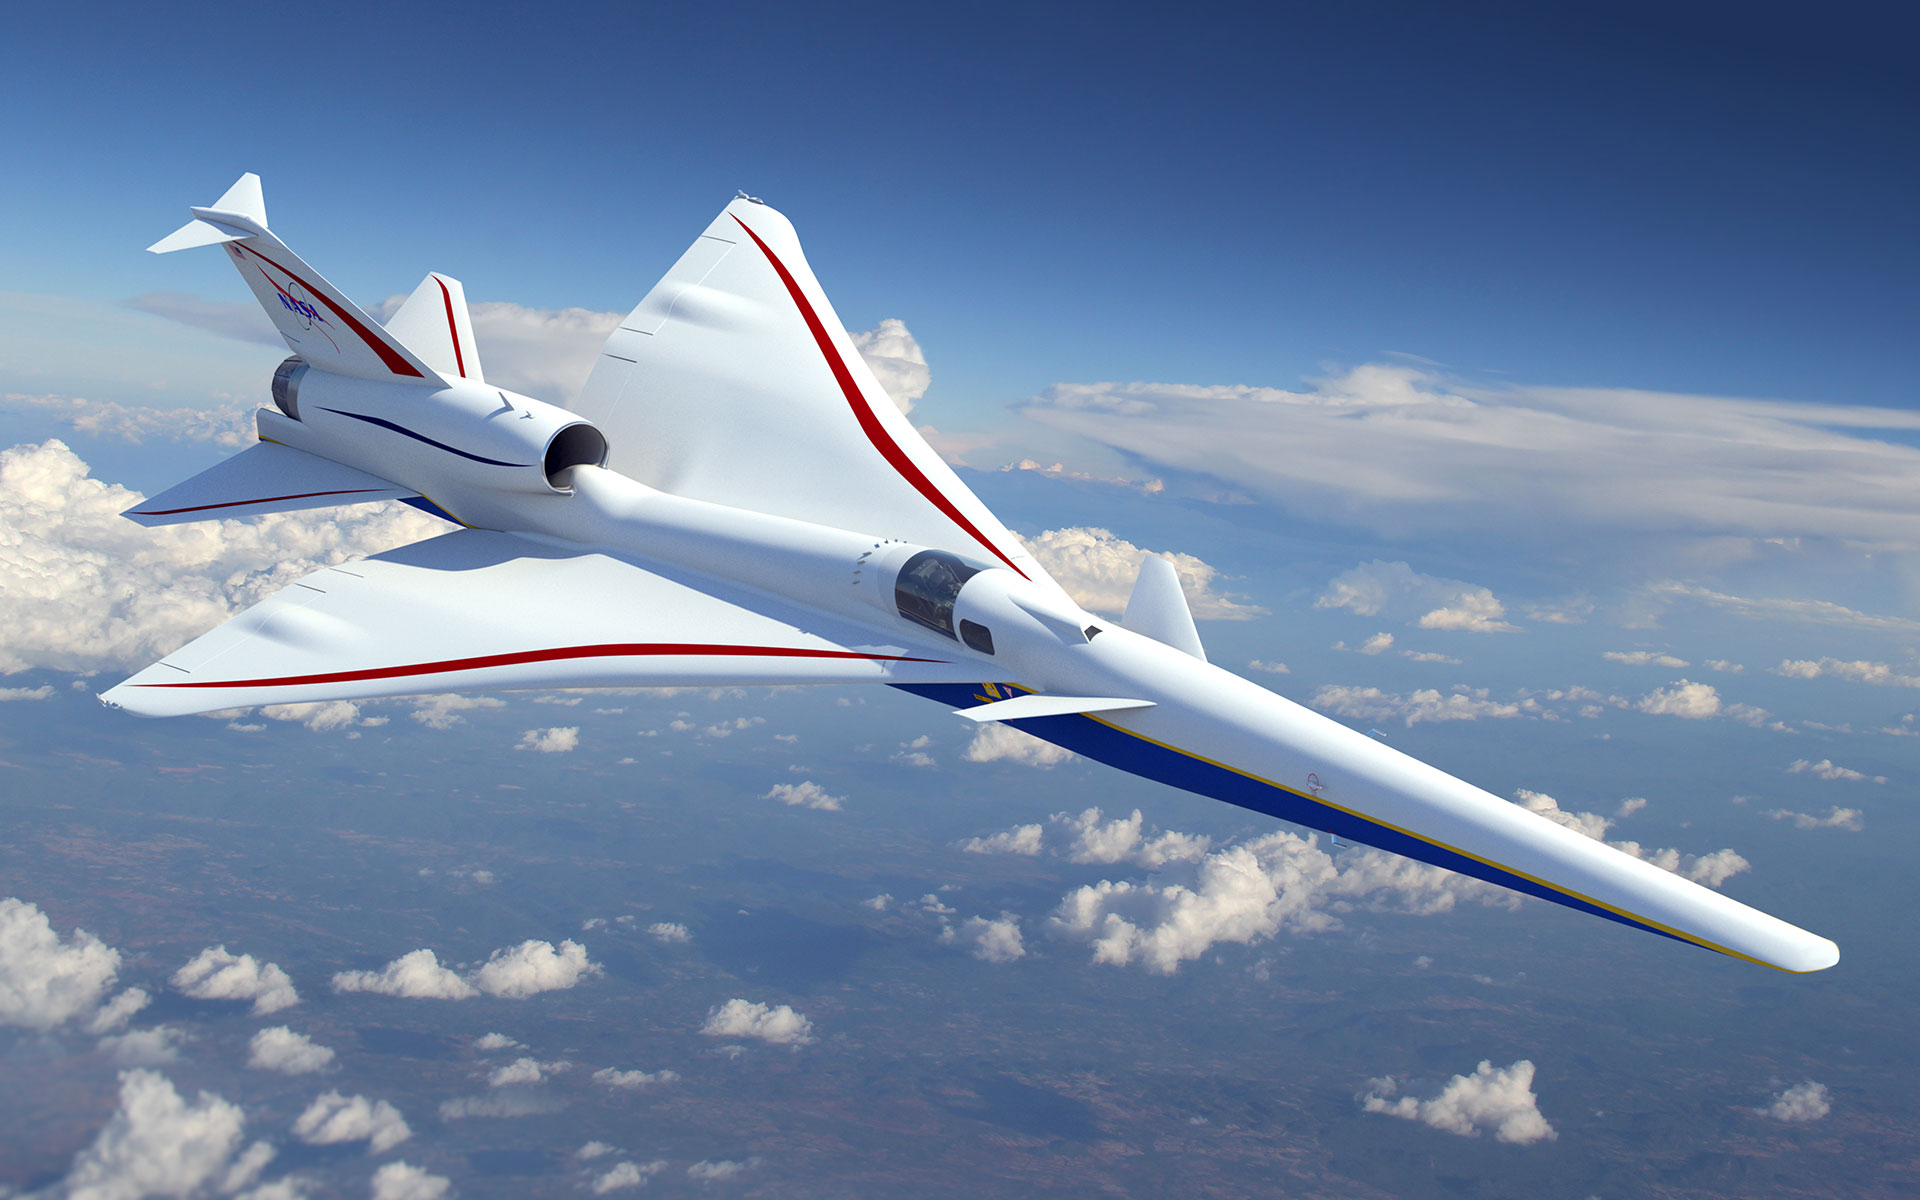
\includegraphics[height=3cm]{../figs/motivation/x59.jpg}};
  \node[anchor=north east, xshift=-2.3cm, yshift=-4.5cm]
    at (current page.north east) {\tiny\color{gray} Source: lockheedmartin.com};
  % https://www.lockheedmartin.com/en-us/products/x-59-quiet-supersonic.html
\end{tikzpicture}

\end{frame}

%---------------------------------------------------------------%

\stepcounter{sectionframecount}
\begin{frame}[t]{Propagation: Pressure Perturbation Solution}

  \begin{tikzpicture}[remember picture,overlay]
    \node[anchor=north east, xshift=-6.3cm, yshift=-2cm]
      at (current page.north east) {%
        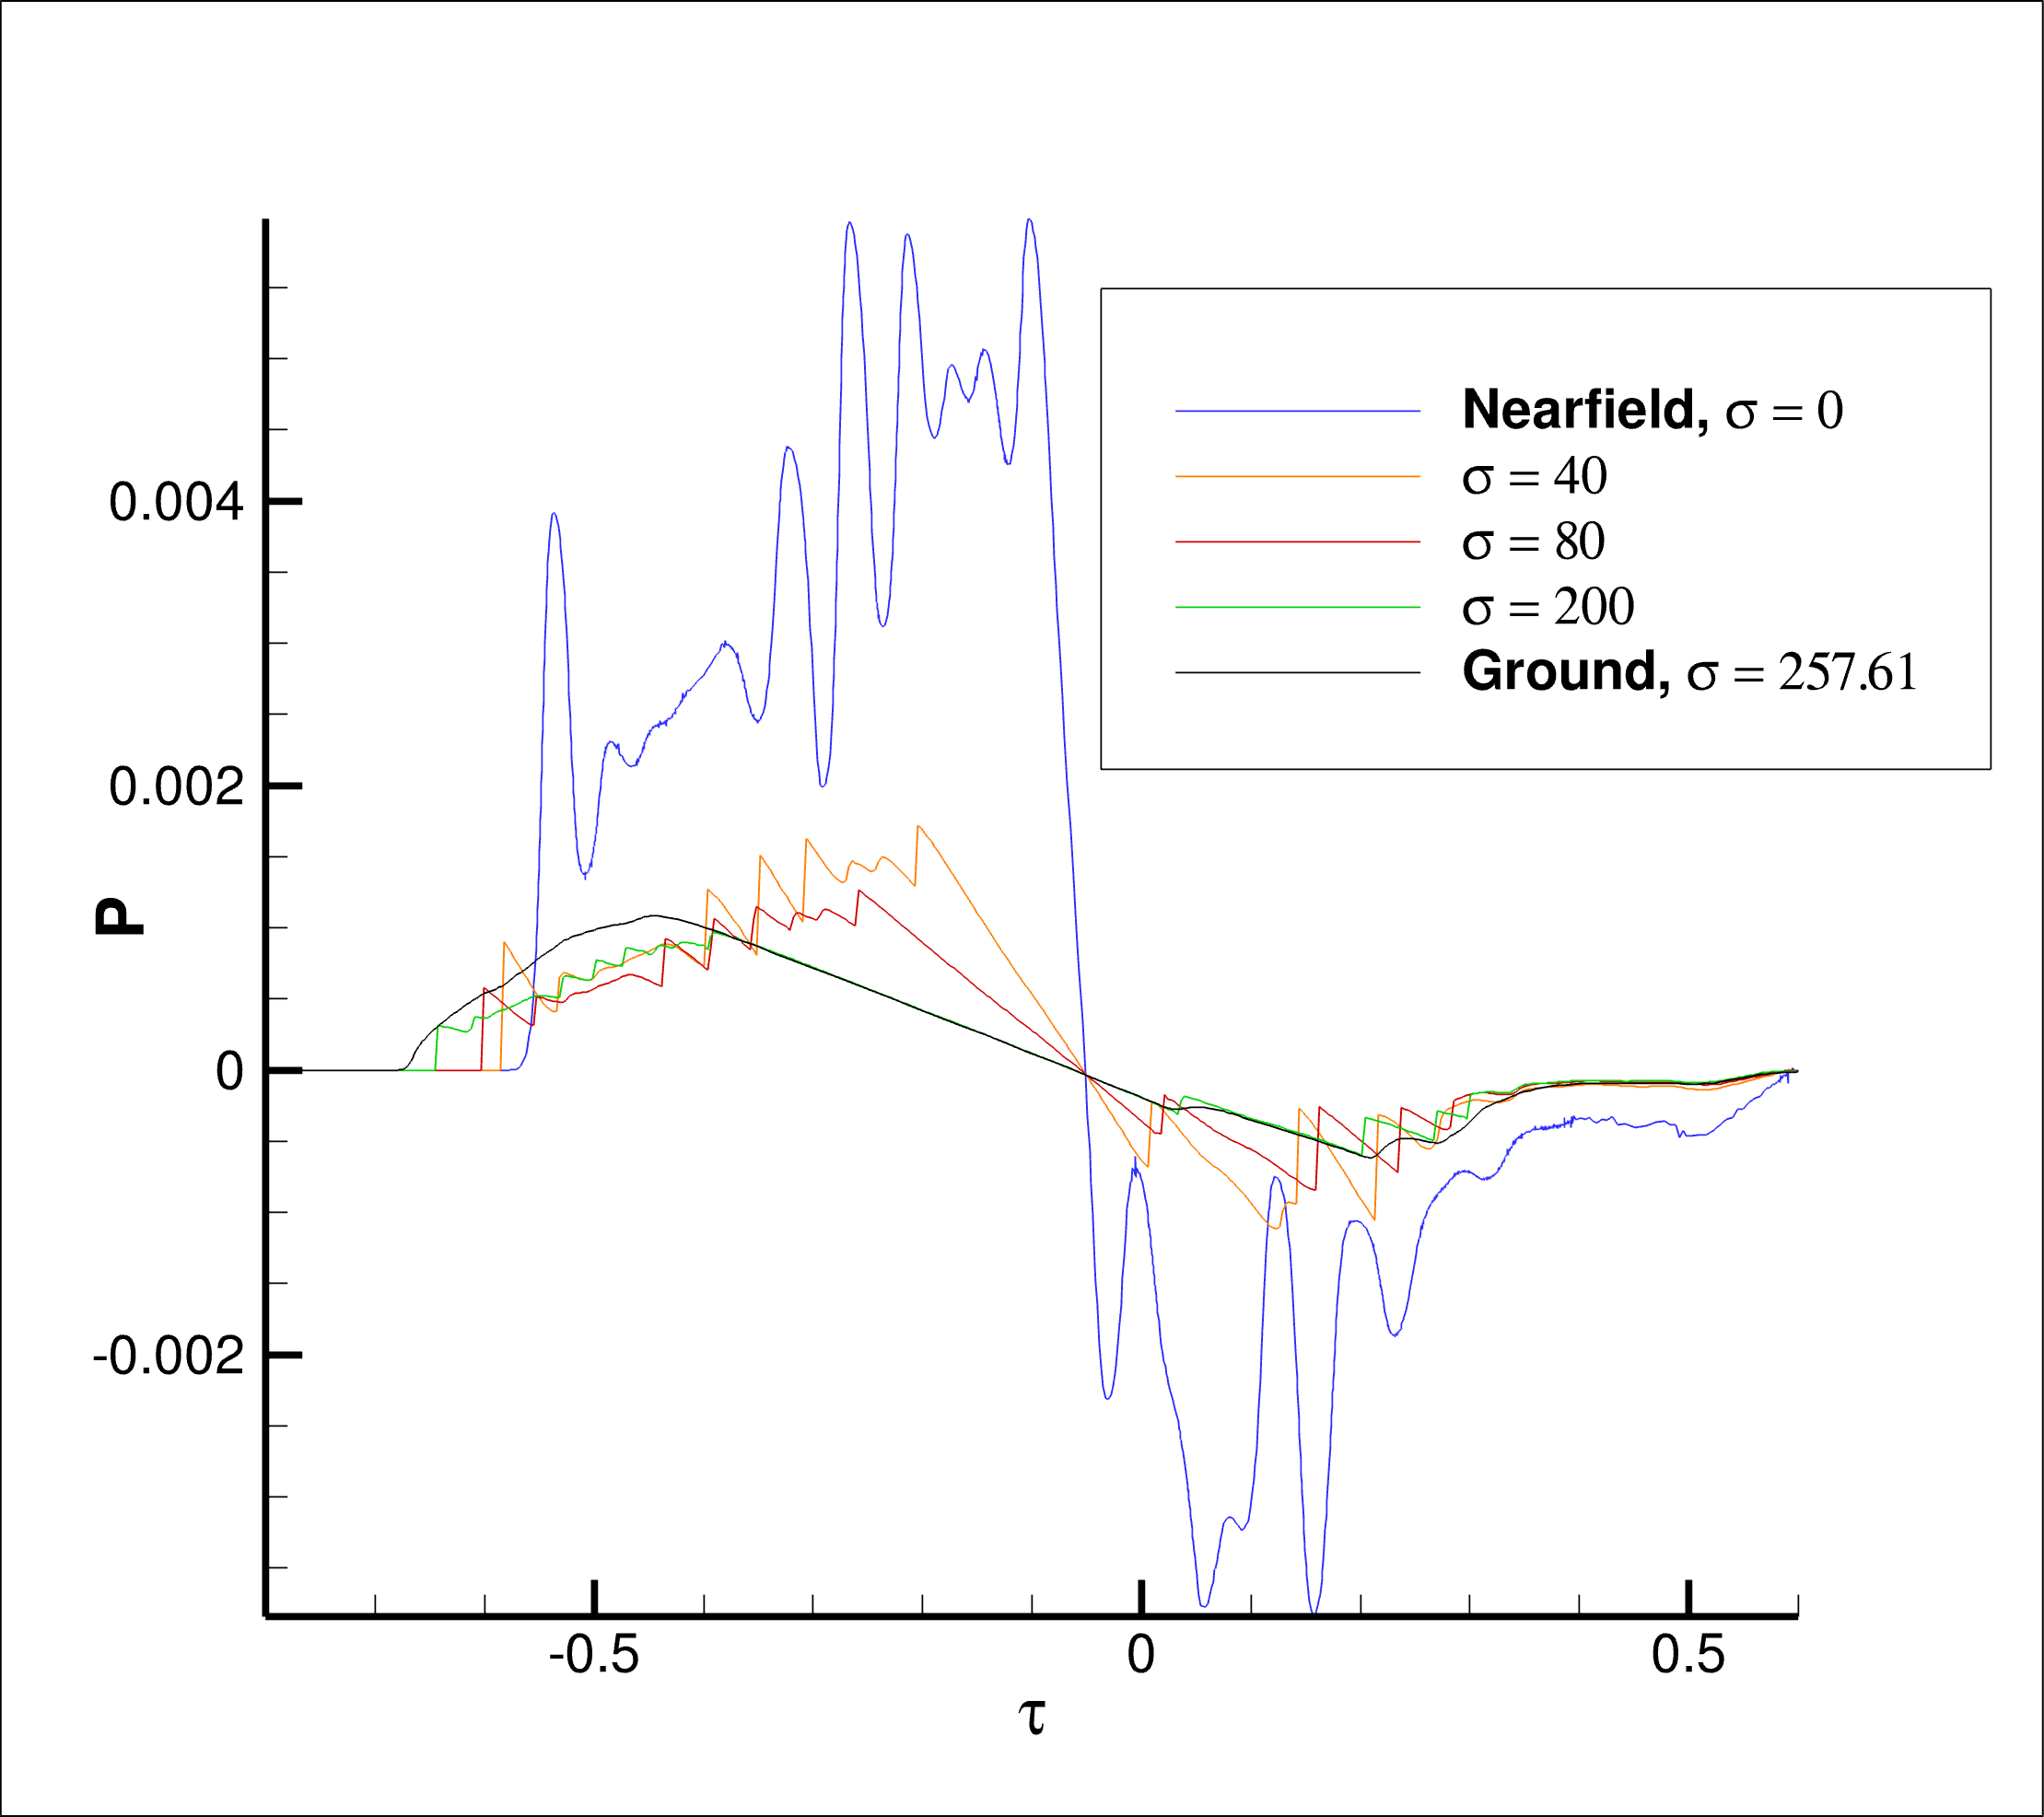
\includegraphics[height=5.8cm, trim=5mm 5mm 5mm 5mm, clip]{../figs/SBW3results/sbw3_P1_128K_P_lines.png}};
  \end{tikzpicture}

  \begin{tikzpicture}[remember picture,overlay]
    \node[anchor=north east, xshift=0.2cm, yshift=-2cm]
      at (current page.north east) {%
        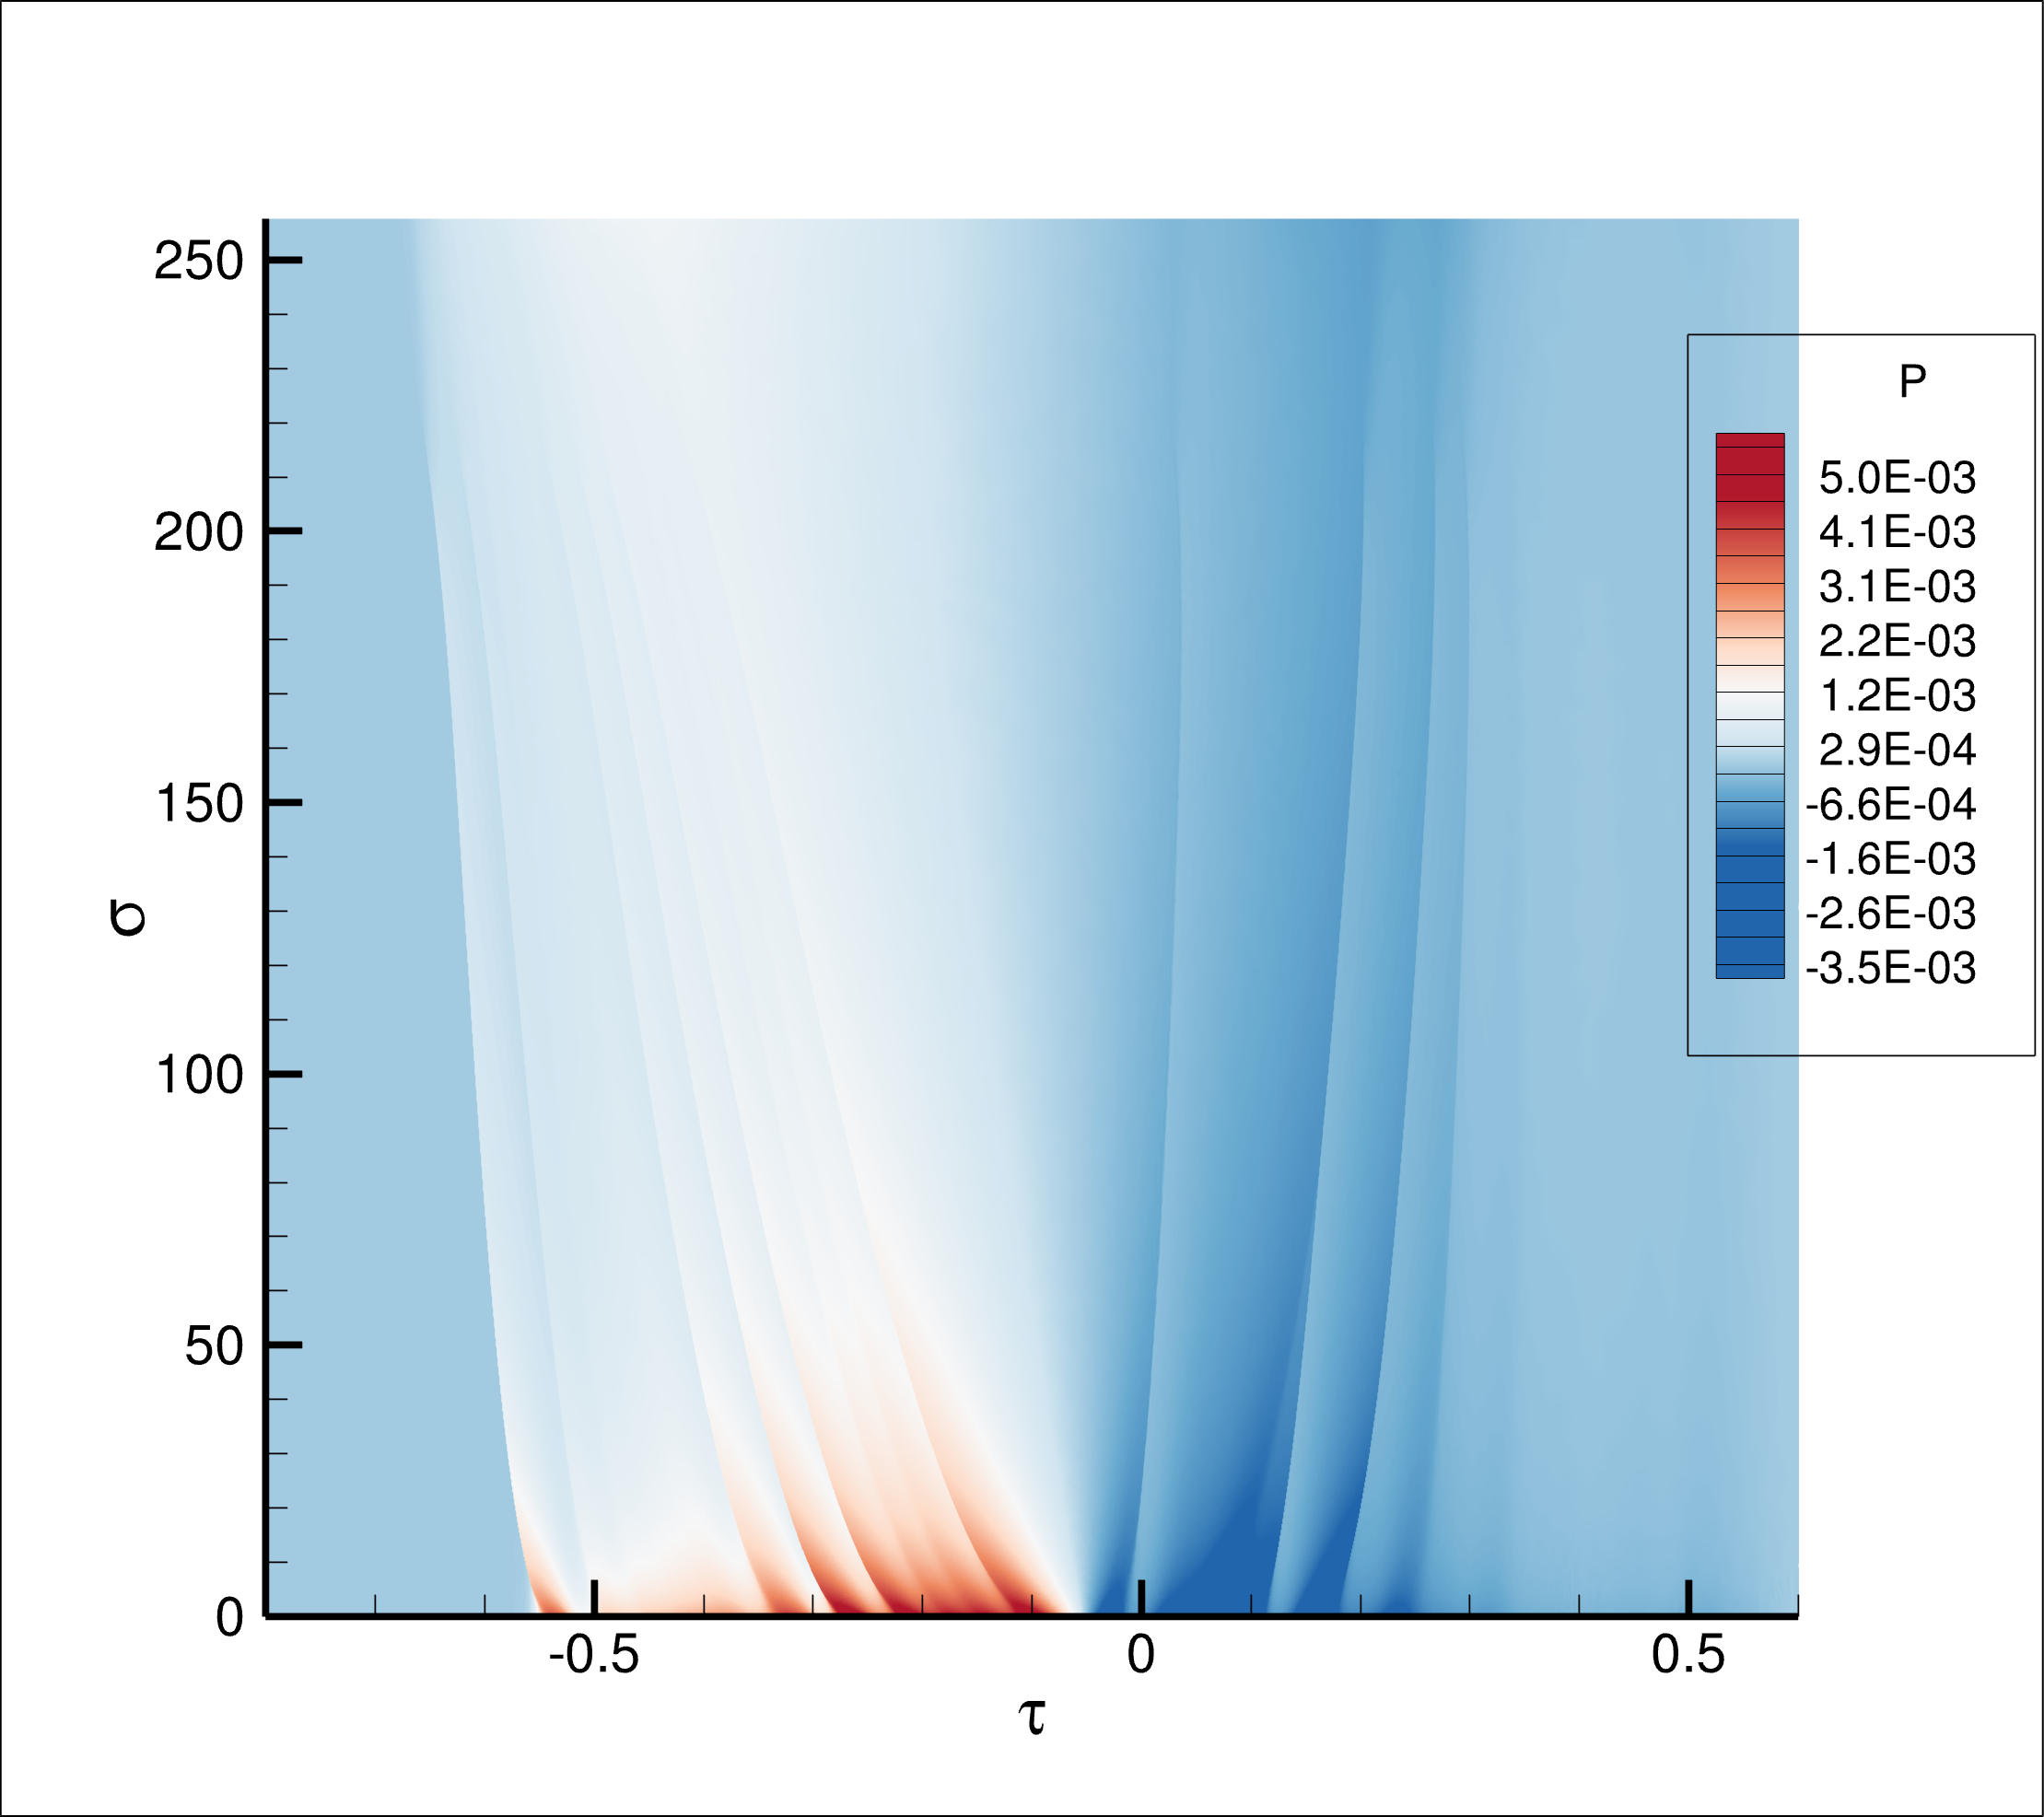
\includegraphics[height=5.8cm, trim=5mm 5mm 5mm 5mm, clip]{../figs/SBW3results/sbw3_P1_128K_P_field.png}};

    % (If you have a defined node 'img' for positioning "Ground" and "Nearfield", make sure it is defined.
    % Otherwise, adjust these nodes accordingly.)
    \node[anchor=south west, font=\scriptsize, black, xshift=83mm, yshift=8mm]
      at (img.north west) {Ground};

    \node[anchor=south west, font=\scriptsize, black, xshift=83mm, yshift=-47.5mm]
      at (img.north west) {Nearfield};
  \end{tikzpicture}

\end{frame}

%---------------------------------------------------------------%

\stepcounter{sectionframecount}
\begin{frame}[t]{Propagation: Evolution Over Adaptive Cycle, 8K Target DOF}

  \centering
  % Clicking on the thumbnail will launch the external video file.
  \href{run:burgers_mesh_and_primal_combined_8K.mp4}{
\includegraphics[width=0.6\linewidth]{../figs/SBW3results/playVideoSymbol.jpg}}

\end{frame}

%---------------------------------------------------------------%

\stepcounter{sectionframecount}
\begin{frame}[t]{Propagation: Final Adapted Mesh for 8K Target DOF}

\begin{tikzpicture}[remember picture,overlay]

  \node[anchor=north east, xshift=-3.5cm, yshift=-1.8cm] at (current page.north east) {%
    \begin{minipage}{0.5\textwidth}
    $p=1$

    \end{minipage}
  };
\end{tikzpicture}

\begin{tikzpicture}[remember picture,overlay]

  \node[anchor=north east, xshift=2.5cm, yshift=-1.8cm] at (current page.north east) {%
    \begin{minipage}{0.5\textwidth}
    $p=2$

    \end{minipage}
  };
\end{tikzpicture}

\begin{tikzpicture}[remember picture,overlay]
  \node[anchor=north east, xshift=-4.5cm, yshift=-2cm]
  at (current page.north east) {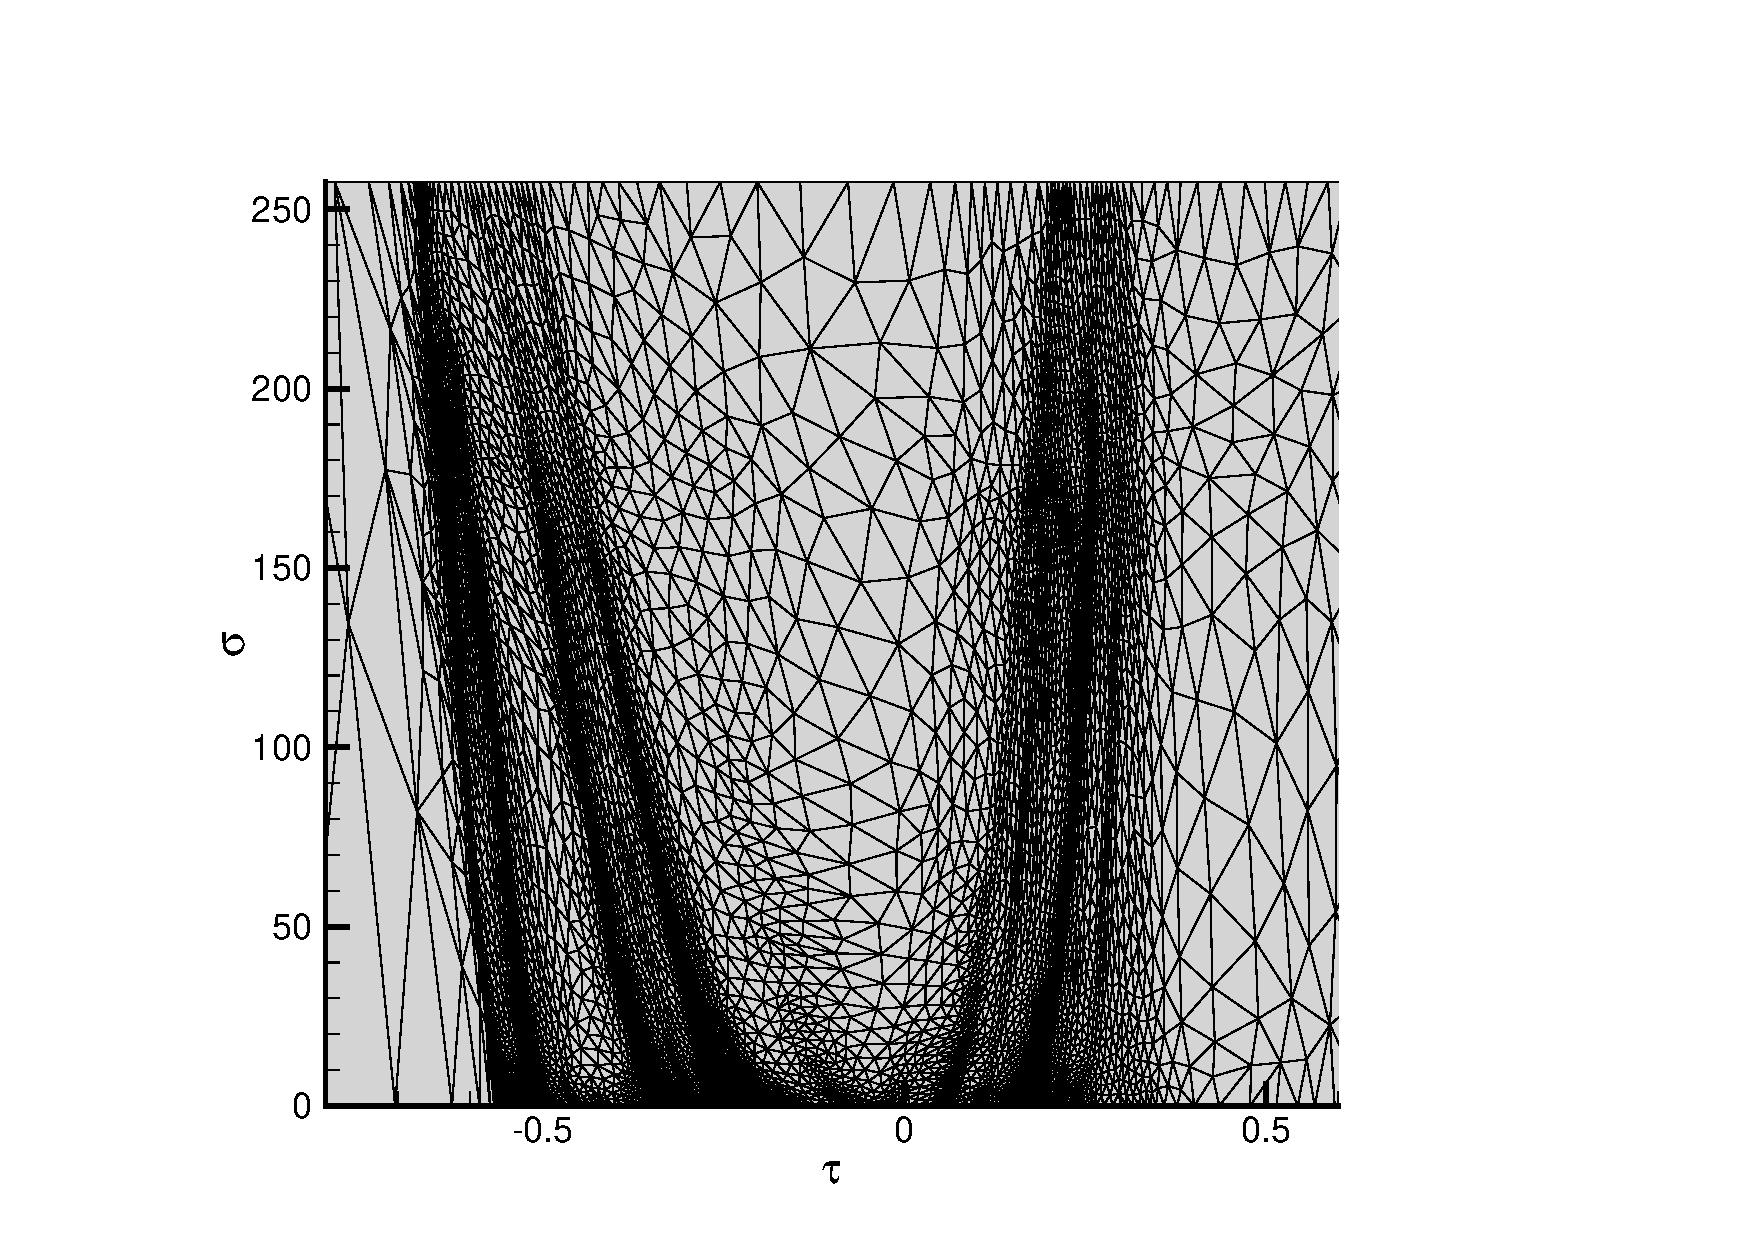
\includegraphics[height=6cm]{../figs/SBW3results/SBW3_P1_8K_mesh_a40_zoomed.pdf}};
\end{tikzpicture}

\begin{tikzpicture}[remember picture,overlay]
  \node[anchor=north east, xshift=1.5cm, yshift=-2cm]
  at (current page.north east) {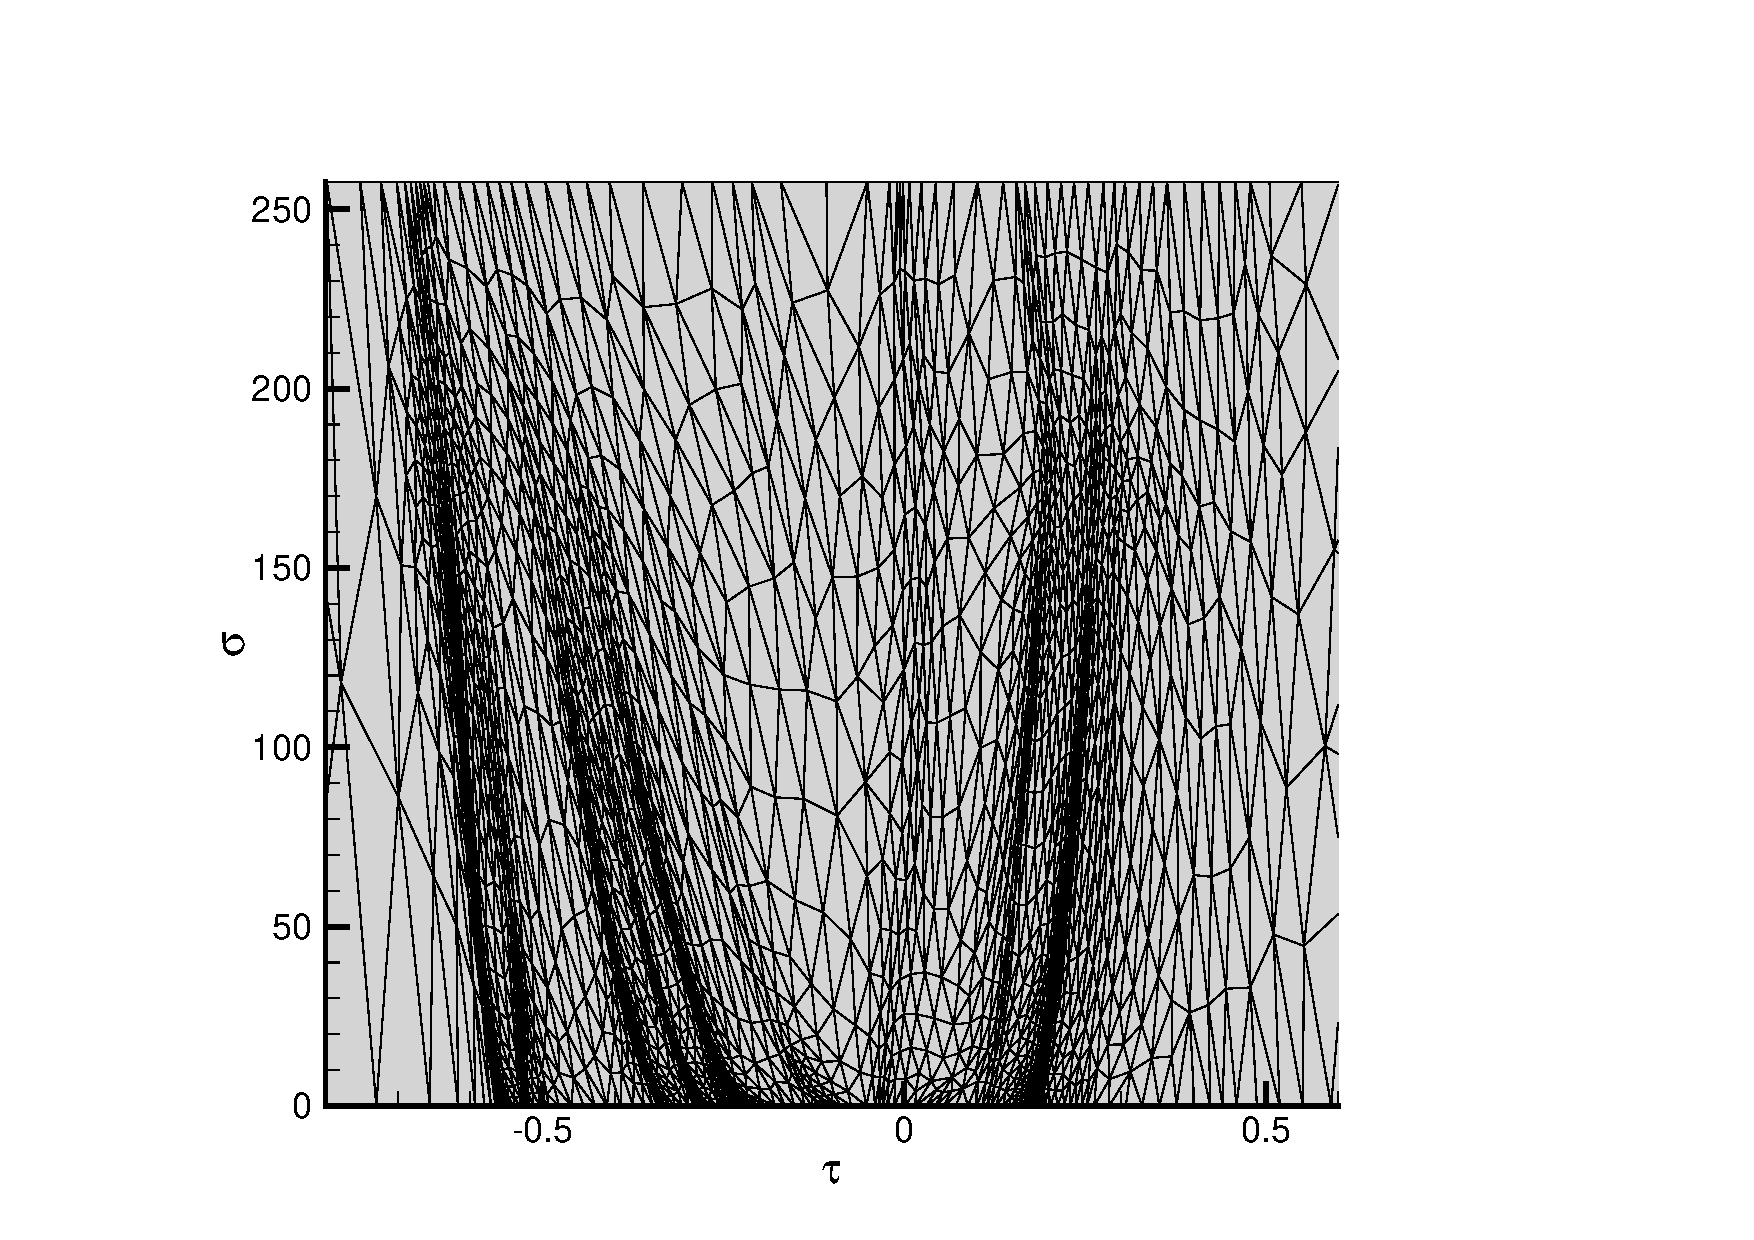
\includegraphics[height=6cm]{../figs/SBW3results/SBW3_P2_8K_mesh_a40_zoomed.pdf}};
\end{tikzpicture}
%
\end{frame}

%---------------------------------------------------------------%

\stepcounter{sectionframecount}
\begin{frame}[t]{Different Adaptation Outputs and Their Adjoints}

  \begin{tikzpicture}[remember picture,overlay]

    \node[anchor=north east, xshift=-6.1cm, yshift=-3cm] at (current page.north east) {%
      \begin{minipage}{0.5\textwidth}
      $\mathcal{J}_{\text{BSEL}}$

      \end{minipage}
    };
  \end{tikzpicture}

  \uncover<2->
  {
  \begin{tikzpicture}[remember picture,overlay]

    \node[anchor=north east, xshift=-6.1cm, yshift=-7cm] at (current page.north east) {%
      \begin{minipage}{0.5\textwidth}
      $\mathcal{J}_p$

      \end{minipage}
    };
  \end{tikzpicture}
  }

  \begin{tikzpicture}[remember picture,overlay]
    \node[anchor=north east, xshift=-6.5cm, yshift=-1.3cm]
    at (current page.north east) {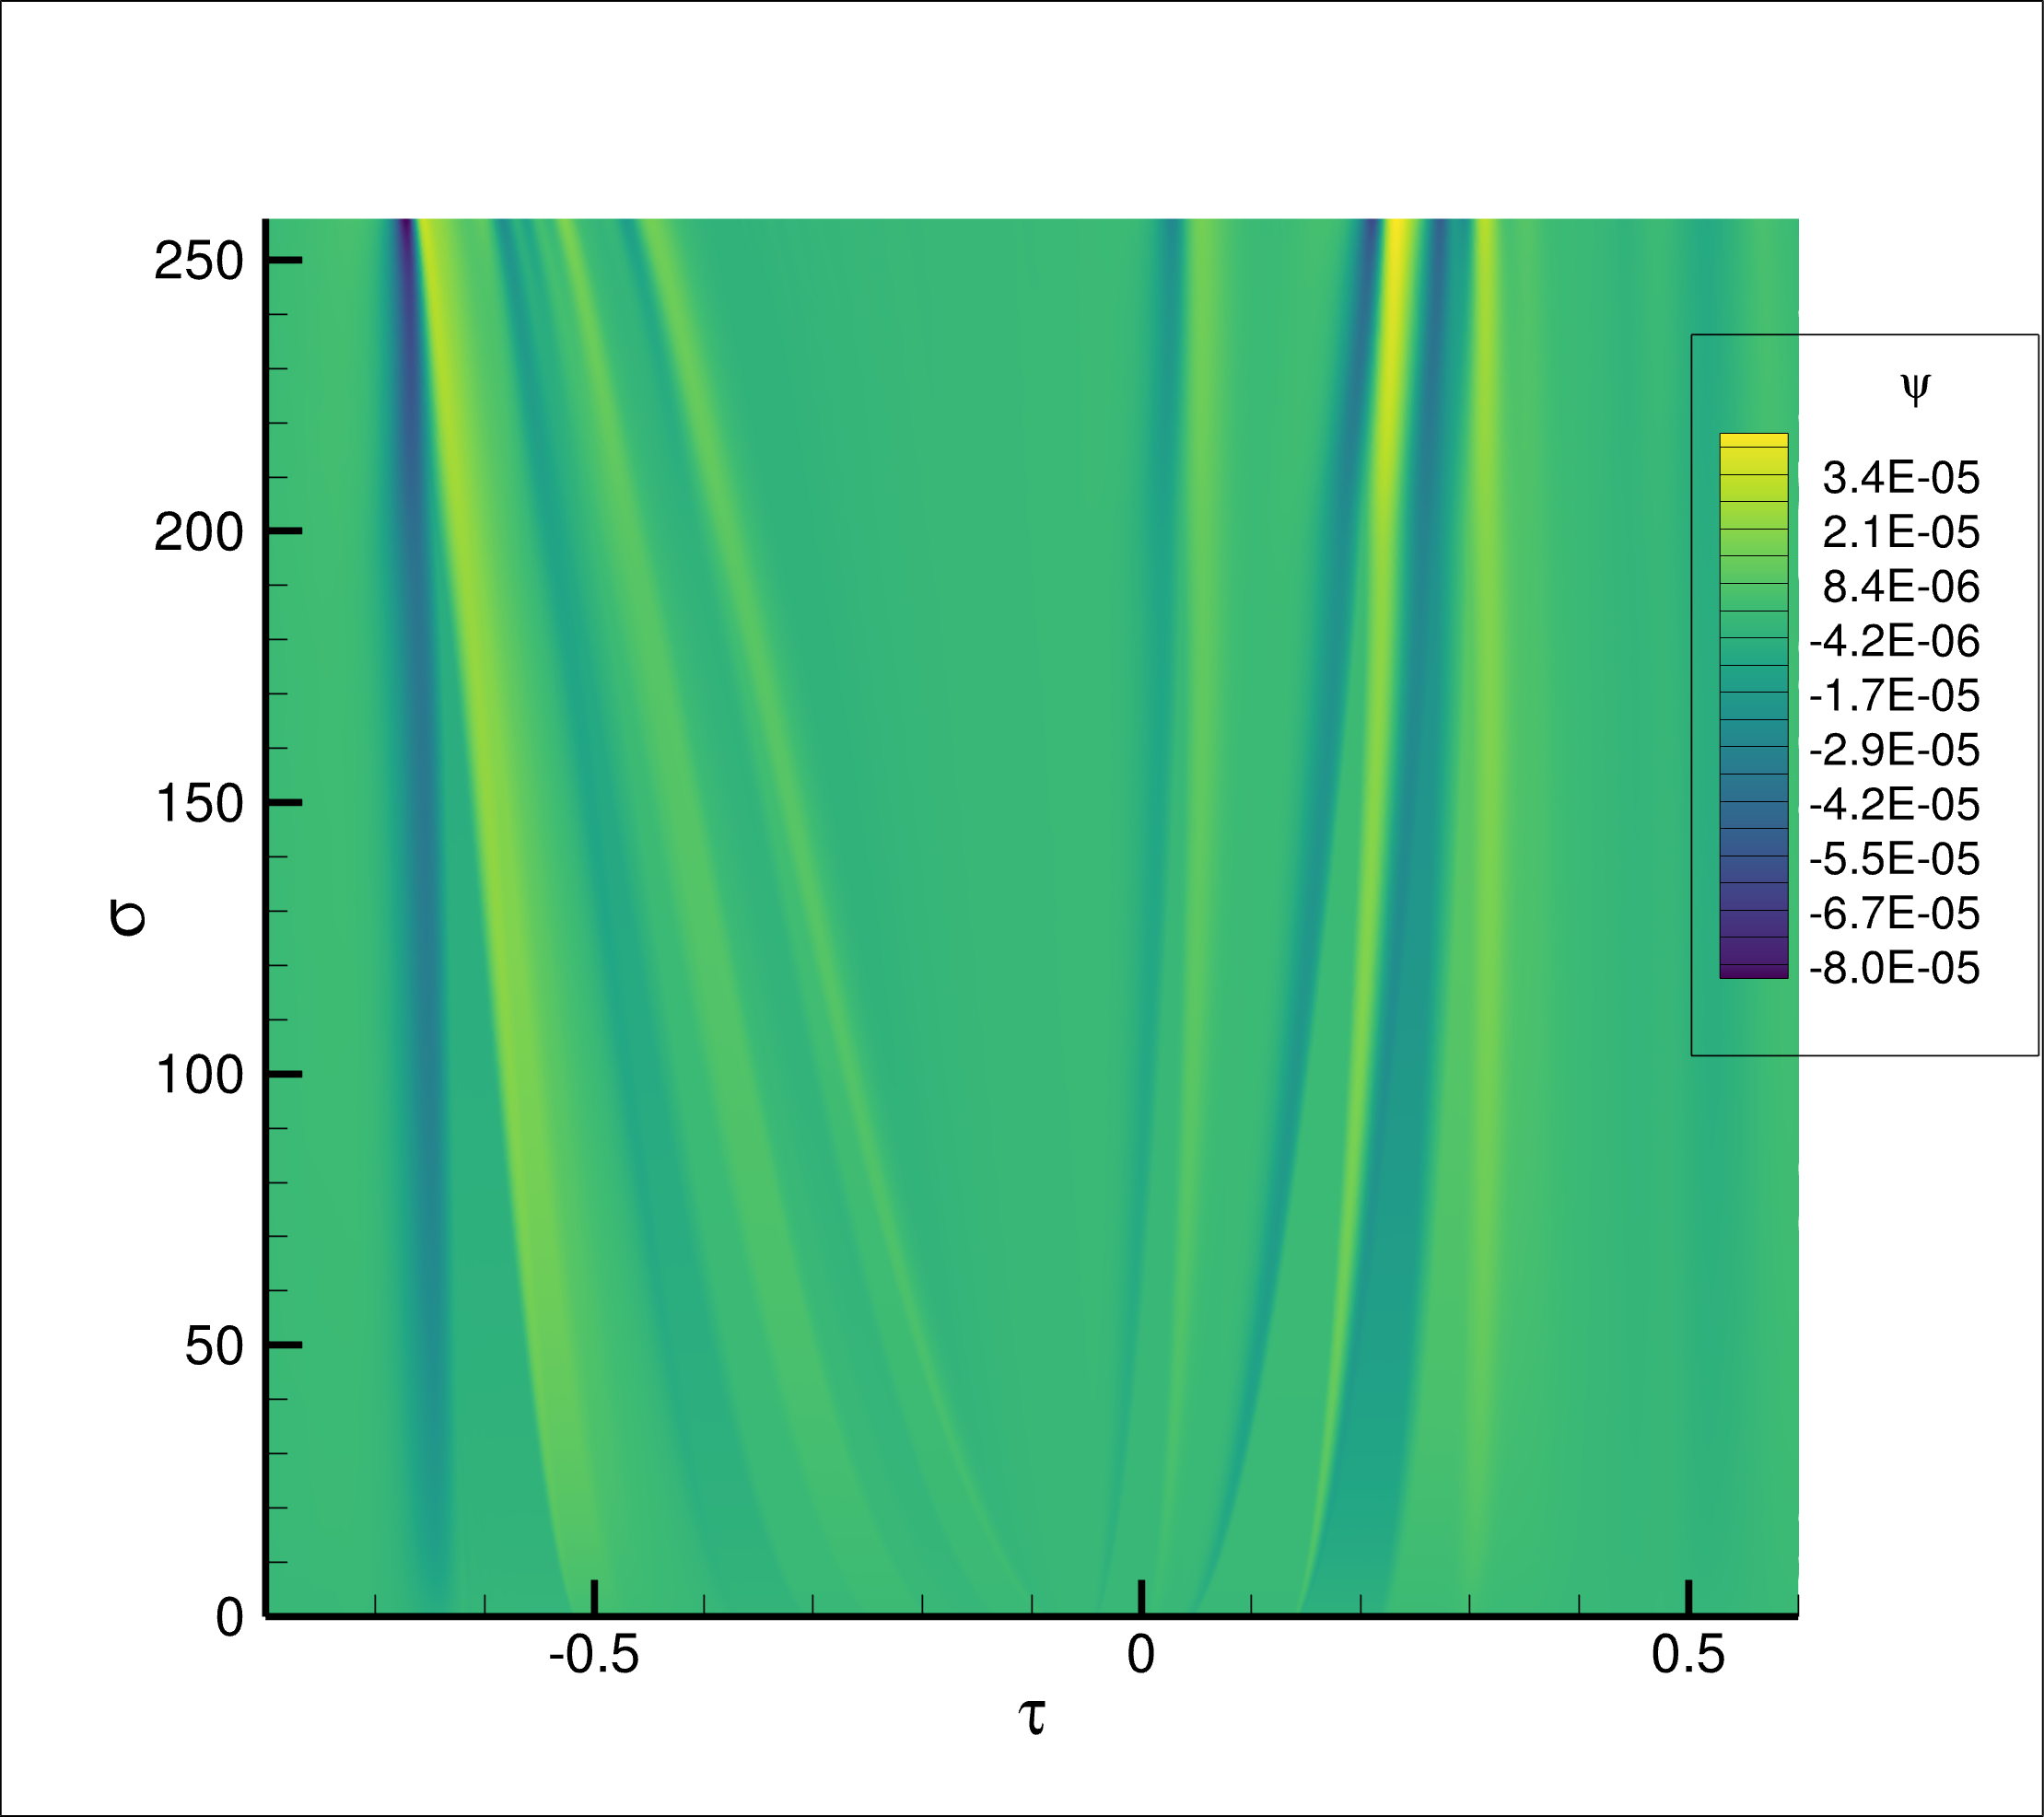
\includegraphics[height=3.9cm, trim=5mm 5mm 2mm 5mm, clip]{../figs/SBW3results/adjointAdaptToBSEL_P2_128K.png}};
  \end{tikzpicture}

  \begin{tikzpicture}[remember picture,overlay]
    \node[anchor=north east, xshift=-0.5cm, yshift=-1.3cm]
    at (current page.north east) {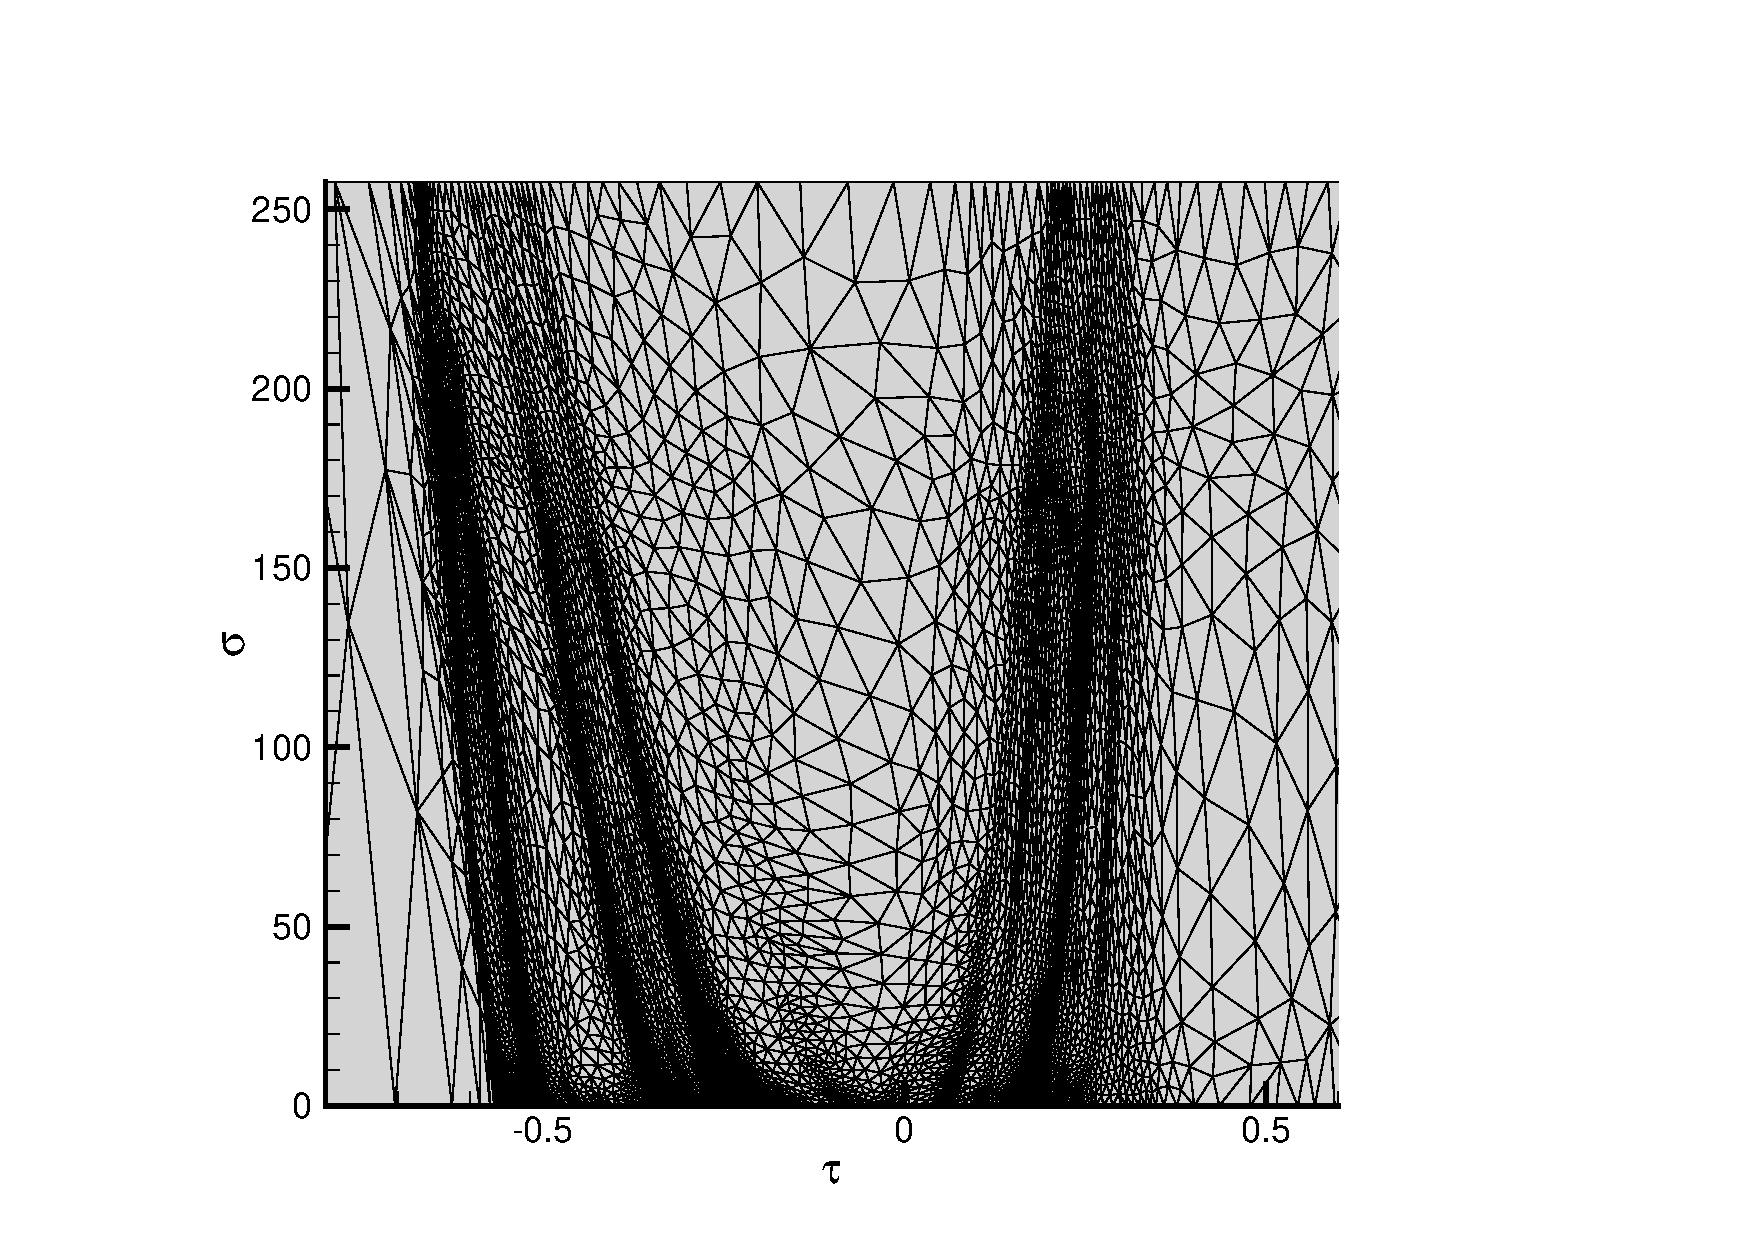
\includegraphics[height=3.9cm]{../figs/SBW3results/SBW3_P1_8K_mesh_a40_zoomed.pdf}};
  \end{tikzpicture}

  \uncover<2->
  {
  \begin{tikzpicture}[remember picture,overlay]
    \node[anchor=north east, xshift=-6.5cm, yshift=-5.1cm]
    at (current page.north east) {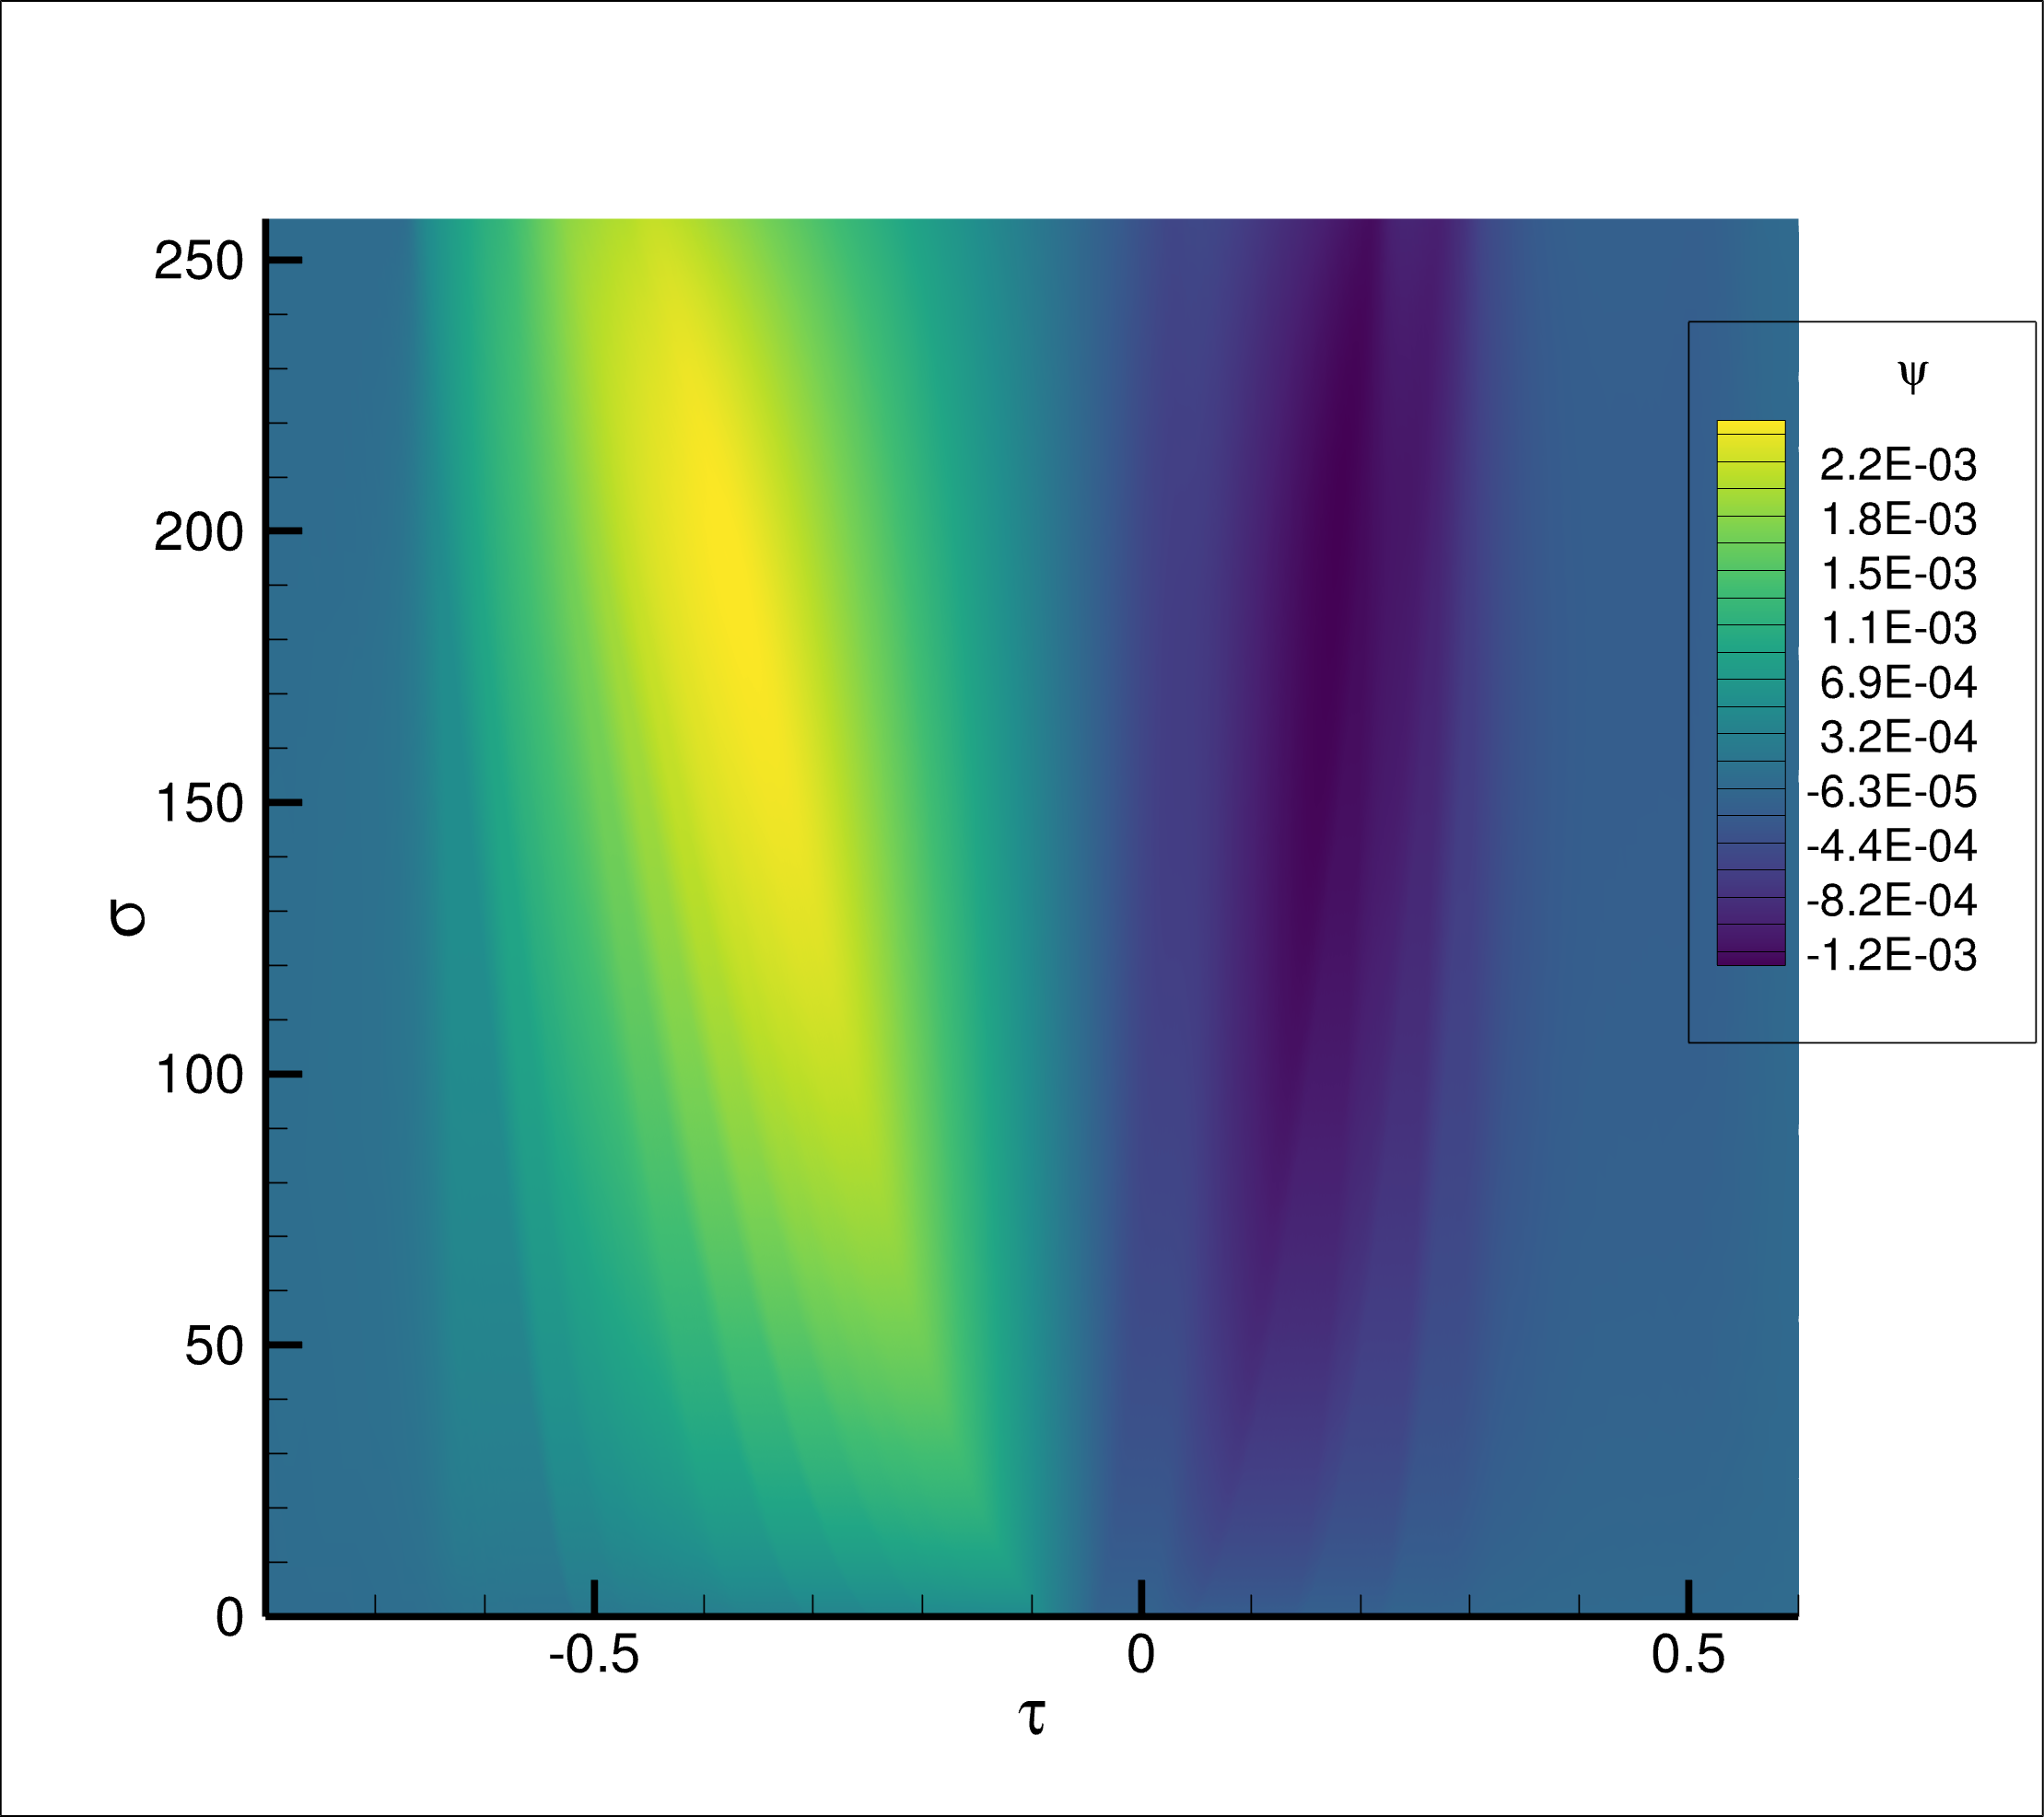
\includegraphics[height=3.9cm, trim=5mm 5mm 2mm 5mm, clip]{../figs/SBW3results/adjointAdaptToP2_P2_128K.png}};
  \end{tikzpicture}

  \begin{tikzpicture}[remember picture,overlay]
    \node[anchor=north east, xshift=-0.5cm, yshift=-5.1cm]
    at (current page.north east) {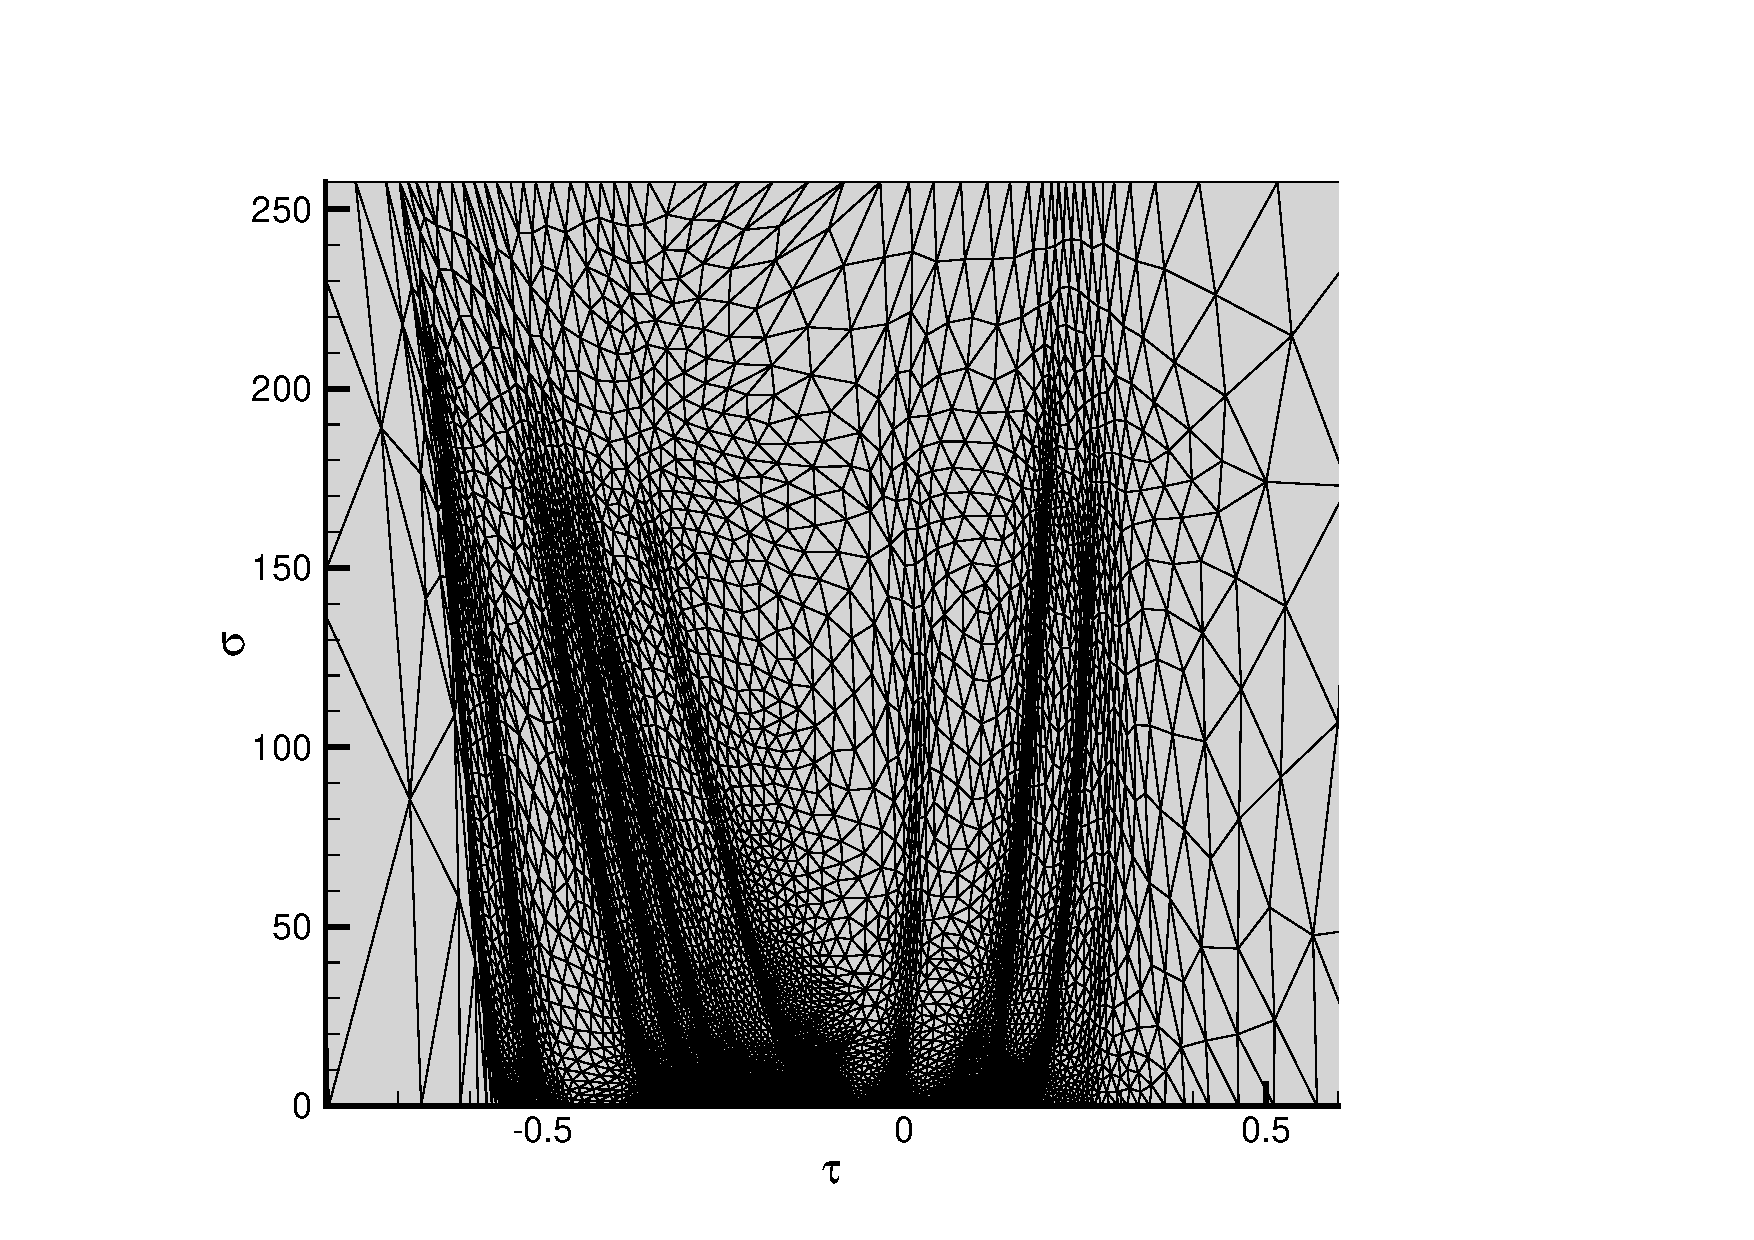
\includegraphics[height=3.9cm]{../figs/SBW3results/SBW3_P1_8K_AdaptToP2_mesh_zoomed.pdf}};
  \end{tikzpicture}
  }
\end{frame}

%---------------------------------------------------------------%

\stepcounter{sectionframecount}
\begin{frame}[t]{At Ground: Pressure Signal and Its Filtering}
\begin{tikzpicture}[remember picture,overlay]

  \node[anchor=north east, xshift=-4.5cm, yshift=-1.4cm] at (current page.north east) {%
    \begin{minipage}{0.5\textwidth}
    Pressure Signal

    \end{minipage}
  };
\end{tikzpicture}

\begin{tikzpicture}[remember picture,overlay]

  \node[anchor=north east, xshift=1.5cm, yshift=-1.4cm] at (current page.north east) {%
    \begin{minipage}{0.5\textwidth}
    B-SEL Filter Output

    \end{minipage}
  };
\end{tikzpicture}

\begin{tikzpicture}[remember picture,overlay]
  \node[anchor=north east, xshift=-6.3cm, yshift=-1.8cm]
  at (current page.north east) {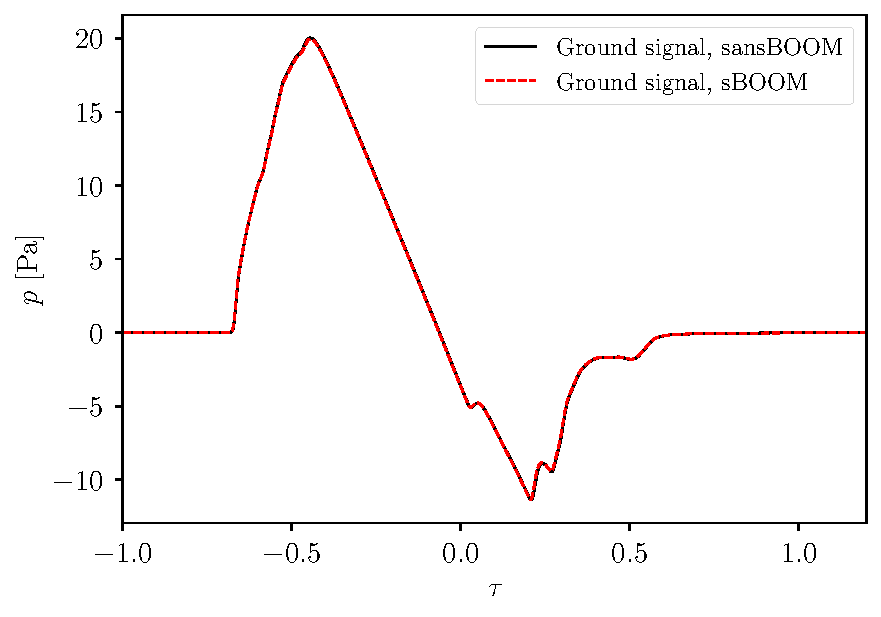
\includegraphics[height=4.3cm]{../figs/SBW3results/ComparisonGround.pdf}};
\end{tikzpicture}

\begin{tikzpicture}[remember picture,overlay]
  \node[anchor=north east, xshift=0.1cm, yshift=-1.8cm]
  at (current page.north east) {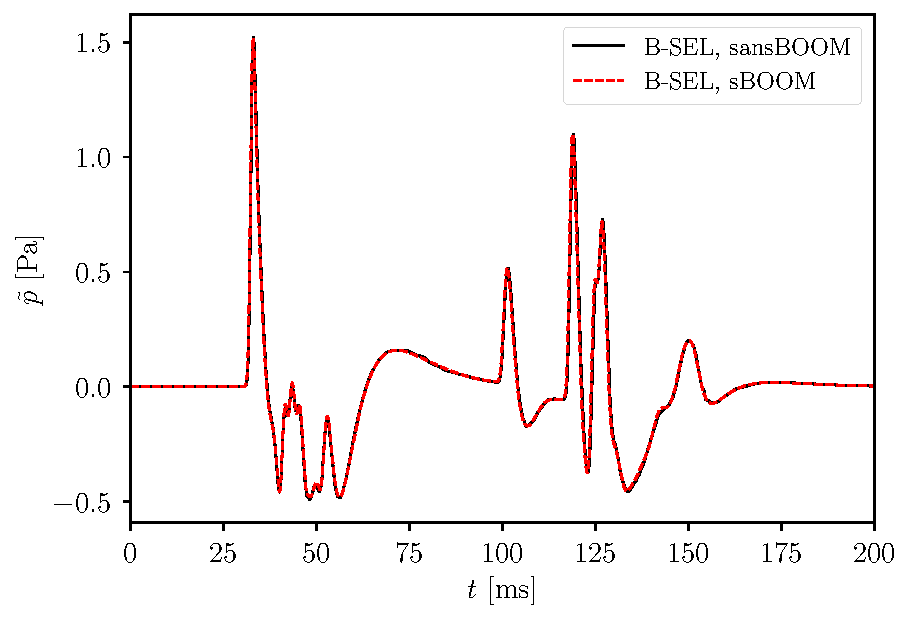
\includegraphics[height=4.3cm]{../figs/SBW3results/comparisonBSEL.pdf}};
\end{tikzpicture}

\uncover<2->
{
\vspace{2.6cm}
\scriptsize Comparison with NASA \textit{sBOOM} code\footnotemark:

}

\uncover<2->
{
\begin{tikzpicture}[remember picture,overlay]
  \node[anchor=north east, xshift=-6.8cm, yshift=-6.7cm] at (current page.north east) {%
    \begin{minipage}{0.45\textwidth}
      \textbf{sansBOOM:}
      \begin{itemize}
        \item Target of 128K DOF in total (space-time).
        \item Total DOF across the $40$ adaptive iterations $\approx 3.2$M DOF.
      \end{itemize}
    \end{minipage}
  };
\end{tikzpicture}

\begin{tikzpicture}[remember picture,overlay]
  \node[anchor=north east, xshift=-1.3cm, yshift=-6.7cm] at (current page.north east) {%
    \begin{minipage}{0.45\textwidth}
      \textbf{sBOOM (NASA, time-marching):}
      \begin{itemize}
        \item \scriptsize 32K DOF in $\tau$ direction.
        \item 39K steps (marching) in $\sigma$ direction.
        \item 1.2B DOF in total (space-time).
      \end{itemize}
    \end{minipage}
  };
\end{tikzpicture}
}

\footnotetext{S. K. Rallabhandi et. al. 2023}
\end{frame}

%---------------------------------------------------------------%

\stepcounter{sectionframecount}
\begin{frame}[t]{At Ground: Loudness Convergence with Mesh Refinement}

\begin{tikzpicture}[remember picture,overlay]

  \node[anchor=north east, xshift=-1.4cm, yshift=-1.8cm] at (current page.north east) {%
    \begin{minipage}{0.5\textwidth}
    B-SEL loudness

    \end{minipage}
  };
\end{tikzpicture}

\begin{tikzpicture}[remember picture,overlay]
  \node[anchor=north east, xshift=-1.8cm, yshift=-2.3cm]
  at (current page.north east) {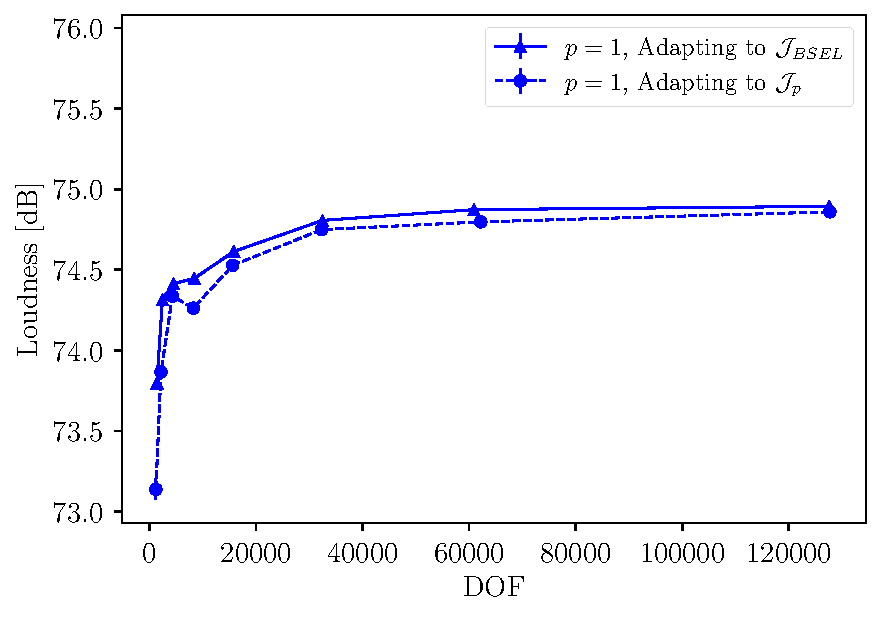
\includegraphics[height=6.5cm]{../figs/SBW3results/loudnessConvergenceForSeminarOnlyP1.pdf}};
\end{tikzpicture}

\uncover<2->
{
\begin{tikzpicture}[remember picture,overlay]
  \node[anchor=north east, xshift=-1.8cm, yshift=-2.3cm]
  at (current page.north east) {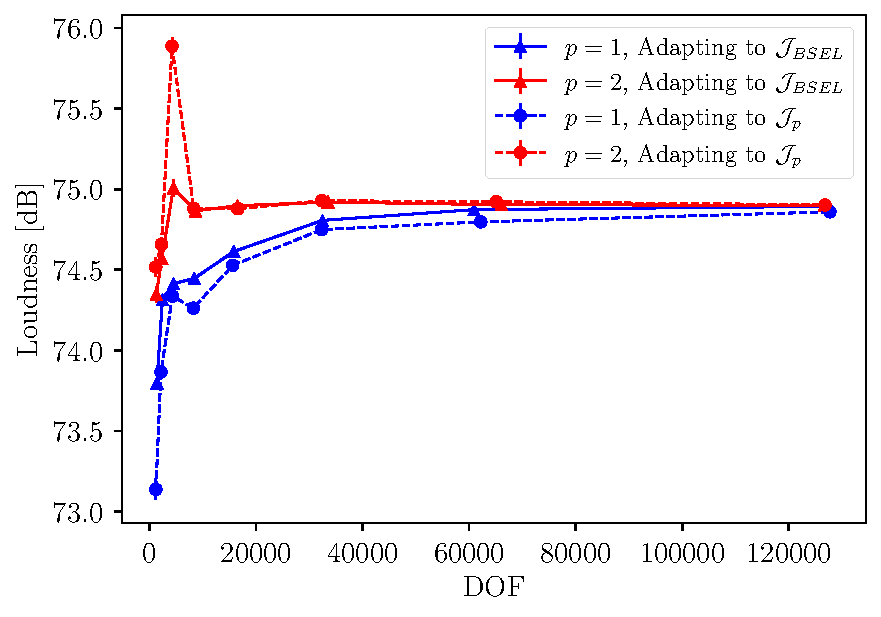
\includegraphics[height=6.5cm]{../figs/SBW3results/loudnessConvergenceForSeminar.pdf}};
\end{tikzpicture}
}

\end{frame}



%=============================================================================%
%=============================================================================%
%=============================================================================%
% Conclusion

% remove the headline
{
\setbeamertemplate{headline}{} % disable headline for this frame only
%---------------------------------------------------------------%

\begin{frame}[t]{Concluding Remarks}
  \textbf{Work completed:}
  \begin{itemize}
    \item Higher-order FEM to solve sonic boom propagation problem.
    \item Unstructured space-time mesh adaptation.
    \item Loudness error estimate driving mesh adaptation.
  \end{itemize}

  \uncover<2->
  {
  \textbf{Outcome:}
  \begin{itemize}
      \item Significant reduction in space-time DOF count, at the expense of solving 2D problem and optimization for the mesh.
      \item The above is highlighted when using higher-order solutions, as quadratic solutions converge the output faster than linear solutions.
    \end{itemize}
  }

  \uncover<3->
  {
    \vspace{15pt}
    \textbf{Ongoing effort:}
    \begin{itemize}
      \item Study convergence of loudness sensitivity to nearfield signal.
    \end{itemize}
  }
\end{frame}

%---------------------------------------------------------------%

\begin{frame}[t]{Acknowledgments}

  \begin{itemize}
    \item This work was supported by funding from NASA (\#80NSSC22K0193) with technical monitor Dr. Sriram Rallabhandi.
    \item The authors gratefully acknowledge technical assistance of NASA specifically from Sriram Rallabhandi, Michael Aftosmis, Marian Nemec, and David Rodriguez.
  \end{itemize}

\end{frame}

}

%---------------------------------------------------------------%

%=============================================================================%
%=============================================================================%
%=============================================================================%
% Thank you slide

\begin{frame}[plain]
  \vfill
  \centering
  {\usebeamerfont{title}\usebeamercolor[fg]{title}Thanks for the attention! \\ \small Questions?}
  \vfill
\end{frame}

%=============================================================================%
%=============================================================================%
%=============================================================================%
% Backup Slides
%=============================================================================%
%=============================================================================%
%=============================================================================%

\appendix

\section{Backup}

\setsectionframes{11}

%---------------------------------------------------------------%

\stepcounter{sectionframecount}
\begin{frame}[t]{Boom Carpet: Front View Schematic}

  \begin{tikzpicture}[remember picture,overlay]
    \node[anchor=north east, xshift=0cm, yshift=-2.8cm]
    at (current page.north east) {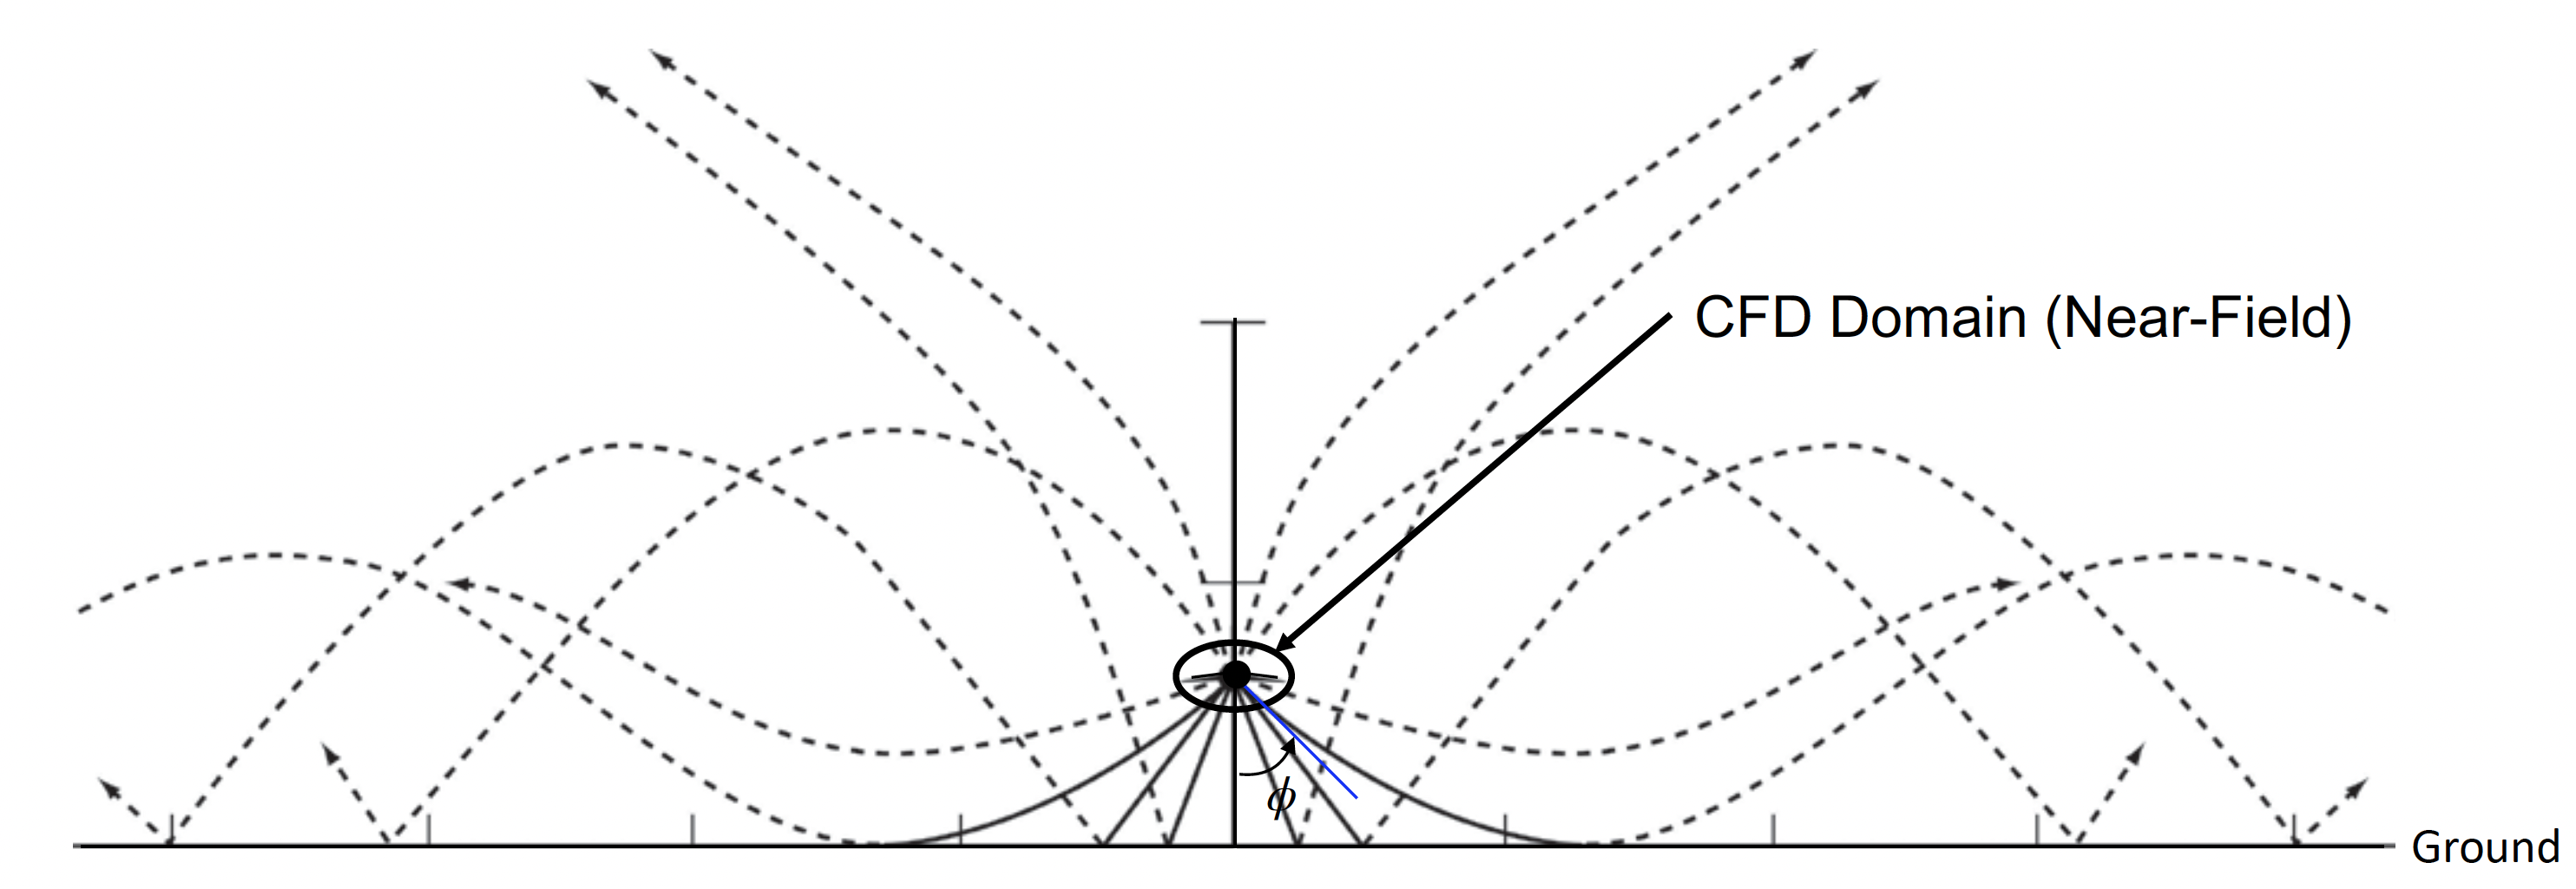
\includegraphics[height=4.3cm]{../figs/backup/boomCarpet.png}};
  \end{tikzpicture}

\end{frame}

%---------------------------------------------------------------%

\stepcounter{sectionframecount}
\begin{frame}[t]{Boom Carpet: Nearfield Conditions and Loudness Values\footnote{S. K. Rallabhandi et. al. 2023}}

  \begin{tikzpicture}[remember picture,overlay]
    \node[anchor=north east, xshift=-6.7cm, yshift=-2.8cm]
    at (current page.north east) {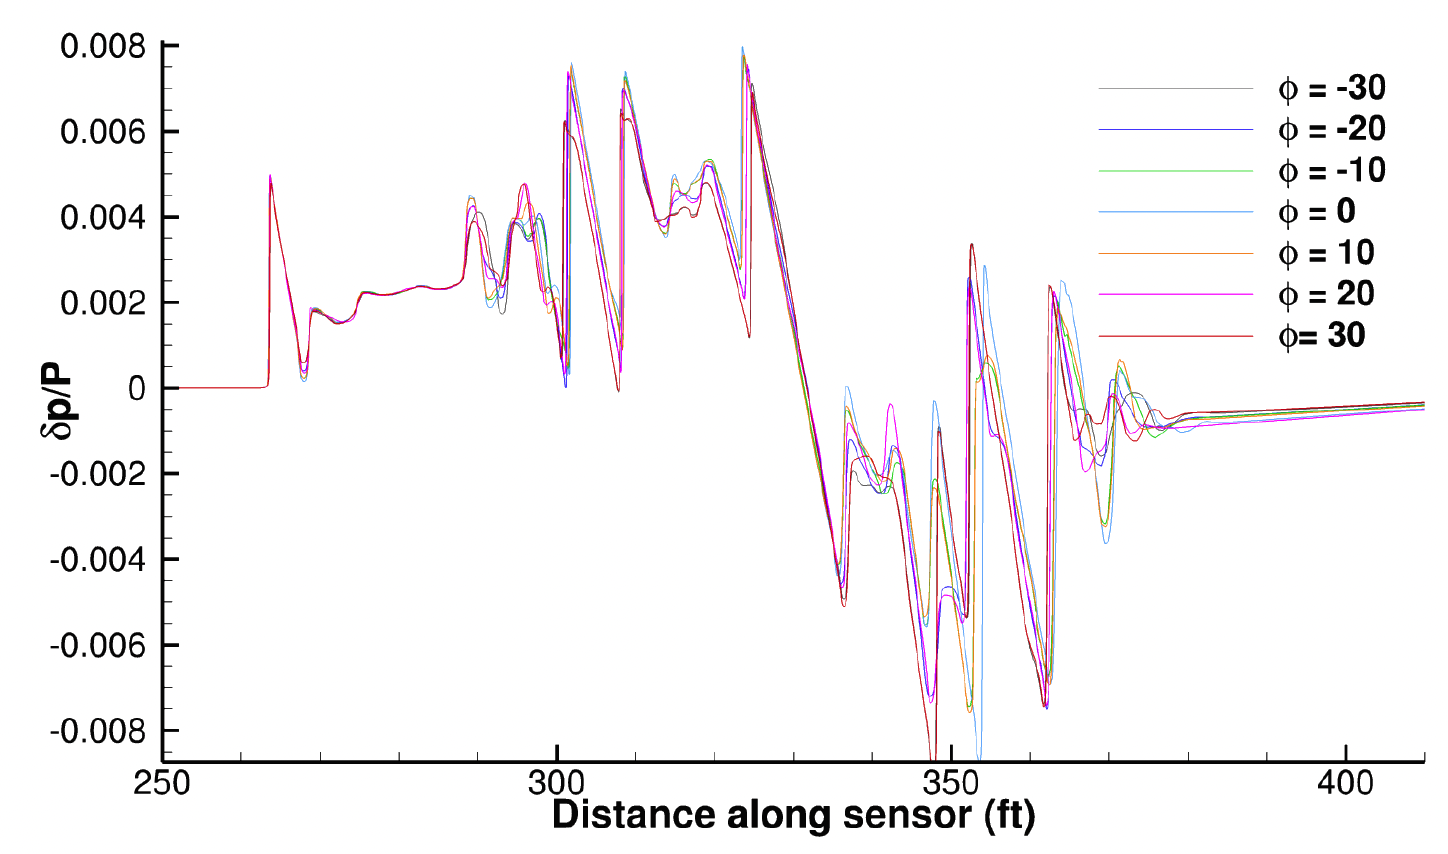
\includegraphics[height=3.5cm]{../figs/backup/nearfieldSeveralPhi.png}};
  \end{tikzpicture}

  \begin{tikzpicture}[remember picture,overlay]
    \node[anchor=north east, xshift=0cm, yshift=-2.8cm]
    at (current page.north east) {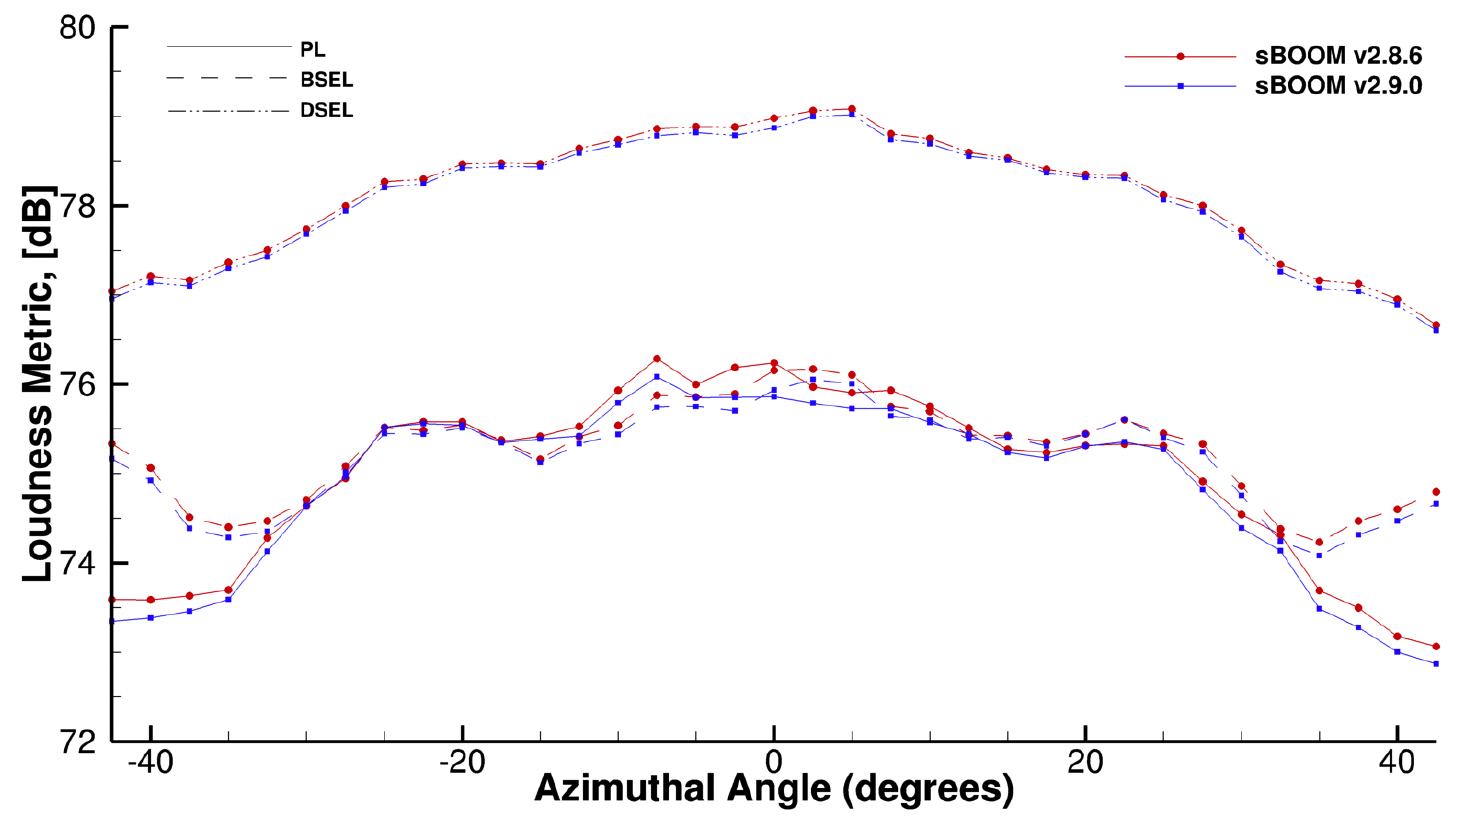
\includegraphics[height=3.5cm]{../figs/backup/loudnessCarpet.png}};
  \end{tikzpicture}

\end{frame}

%---------------------------------------------------------------%

\stepcounter{sectionframecount}
\begin{frame}[t]{Atmosphere Model: Standard}

Atmosphere model refers to how the atmospheric properties depend on altitude.

\textbf{Standard model:} First two layers:

\begin{tikzpicture}[remember picture,overlay]
  \node[anchor=north east, xshift=-5.5cm, yshift=-3.5cm]
  at (current page.north east) {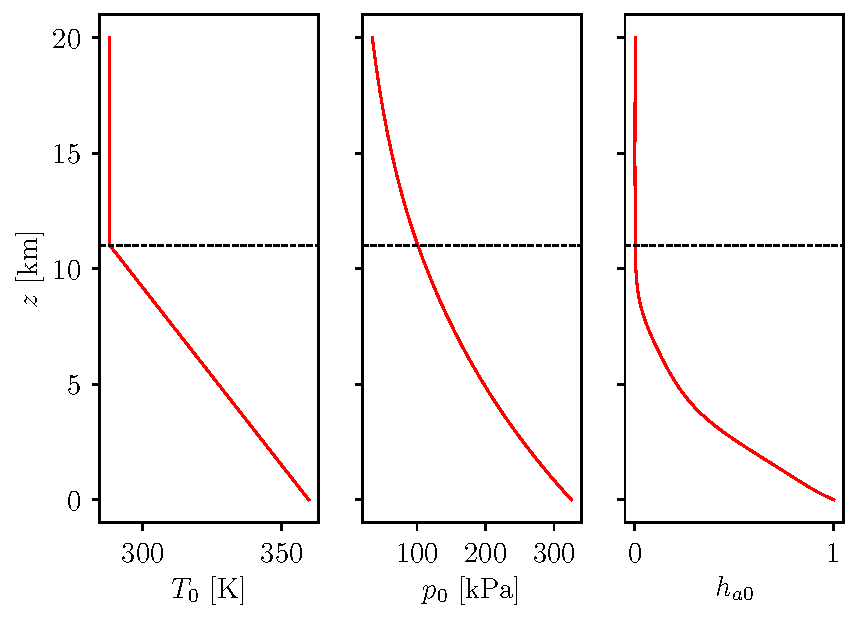
\includegraphics[height=5.0cm]{../figs/boom_modeling/atmosphereStandard.pdf}};
\end{tikzpicture}


\begin{tikzpicture}[remember picture,overlay]
  \node[anchor=north east, xshift=-0.2cm, yshift=-2.8cm] at (current page.north east) {%
    \begin{minipage}{0.4\textwidth}
      \textbf{Additionally, models for:}
      \par\medskip
      \begin{itemize}
        \item Density and speed of sound: $\rho_0$, $c_0$,
        \item Gol'berg number: $\Gamma$,
        \item Relaxation coefficients: $C_\nu, \theta_\nu$,
        \item Ray tube area: $A_{n0}$,
      \end{itemize}

      as functions of atmospheric properties.
    \end{minipage}
  };
\end{tikzpicture}

\end{frame}
%---------------------------------------------------------------%

\stepcounter{sectionframecount}
\begin{frame}[t]{Variational Multiscale with Discontinuous Subscales (VMSD) Method}
  % \vspace{pt}
  \textbf{Discretization of $\Omega$:}

  \vspace{5pt}
  $\mathcal{T}_h := \{\kappa\}_{\kappa = 1}^K$ is a triangulation of the domain $\Omega$ into $K$ elements.


  \vspace{10pt}
  \textbf{Propose solution:}

  $\boldsymbol{u}_h := \bar{\boldsymbol{u}}_{h,p} + \boldsymbol{u}_{h,p^\prime}^\prime$, ~~~~$\bar{\boldsymbol{u}}_{h,p} \in \overline{\mathcal{V}}_{h,p}$,~~ $\boldsymbol{u}^\prime_{h,p^\prime} \in \mathcal{V}^\prime_{h,p^\prime}$.

  \vspace{10pt}
  \textbf{VMSD solution spaces:}

  \vspace{-15pt}
  \begin{equation}
    \text{(\textit{Coarse} scale) } \overline{\mathcal{V}}_{h,p} := \{\boldsymbol{v}\in [C^0(\Omega)]^m : \boldsymbol{v}|_\kappa \in [\mathcal{P}^p(\kappa)]^m, \forall \kappa \in \mathcal{T}_h\},
  \end{equation}

  \vspace{-15pt}
  \begin{equation}
    \text{(\textit{Fine} scale) } \mathcal{V}^\prime_{h,p^\prime} := \{\boldsymbol{v}\in [L^2(\Omega)]^m : \boldsymbol{v}|_\kappa \in [\mathcal{P}^{p^\prime}(\kappa)]^m, \forall \kappa \in \mathcal{T}_h\}.
  \end{equation}

\end{frame}

%---------------------------------------------------------------%

\stepcounter{sectionframecount}
\begin{frame}[t]{Variational Multiscale with Discontinuous Subscales (VMSD) Method}
  \textbf{Weak statement:}

  \vspace{10pt}
  \textbf{Find $(\bar{\boldsymbol{u}}_{h,p}$, $\boldsymbol{u}^\prime_{h,p^\prime}) \in \overline{\mathcal{V}}_{h,p} \times \mathcal{V}^\prime_{h,p^\prime}$ such that:}
  \begin{equation}
    \mathcal{R}(\bar{\boldsymbol{v}}_{h,p},\boldsymbol{v}^\prime_{h,p^\prime};\bar{\boldsymbol{u}}_{h,p},\boldsymbol{u}^\prime_{h,p^\prime}) = 0,~~\forall (\bar{\boldsymbol{v}}_{h,p},\boldsymbol{v}^\prime_{h,p^\prime}) \in \overline{\mathcal{V}}_{h,p} \times \mathcal{V}^\prime_{h,p^\prime}.
    \label{e:multiscale_weak_statement}
  \end{equation}

  \vspace{10pt}
  \textbf{Remarks:}
  \begin{itemize}
    \item $\boldsymbol{u}^\prime_{h,p^\prime}$ DOFs are element-wise decoupled. Thus, they can be static condensed and the total cost becomes the same as a CG method.
    \item For same accuracy requirement, more efficient (less DOFs) than CG and DG.
    \item Adjoint consistent.
  \end{itemize}
\end{frame}

%---------------------------------------------------------------%

\stepcounter{sectionframecount}
\begin{frame}[t]{Shock Indicator $s_{\text{grad}}$}

  Starting point:
  \begin{equation}
    \xi := \dfrac{H_{\tau\tau}}{p} \left|\dfrac{\partial P}{\partial \tau}\right|,~~~\hat{\xi} = \dfrac{\xi}{\xi_1},
  \end{equation}
  then:
  \begin{equation}
    s_\text{grad} := s_\text{grad}(\hat{\xi}) = \dfrac{\hat{\xi} [\tanh(p^2\hat{\xi})]^{p-1}}{1+\exp\left[-k \left(\hat{\xi} - \alpha(p)\right)\right]},
    \label{e:s_grad}
  \end{equation}
  where $k,\alpha(p) \in \mathbb{R}$.
\end{frame}

%---------------------------------------------------------------%

\stepcounter{sectionframecount}
\begin{frame}[t]{Shock Indicator $s_{\text{grad}}$}
  \vspace{-10pt}
  \begin{equation}
    \small
    s_\text{grad} := s_\text{grad}(\hat{\xi}) = \dfrac{\hat{\xi} [\tanh(p^2\hat{\xi})]^{p-1}}{1+\exp\left[-k \left(\hat{\xi} - \alpha(p)\right)\right]},
    \label{e:s_grad}
  \end{equation}

  \begin{tikzpicture}[remember picture,overlay]
    \node[anchor=north east, xshift=-2.5cm, yshift=-3.2cm]
    at (current page.north east) {\includegraphics[height=5.7cm]{../figs/shock_capturing/s_grad.pdf}};
  \end{tikzpicture}
  \end{frame}


%---------------------------------------------------------------%

\stepcounter{sectionframecount}
\begin{frame}[t]{Test With Smooth Problem}
\vspace{-10pt}
Smooth problem with available exact solution:

\begin{itemize}
  \item Solve without artificial viscosity.
  \item Solve with artificial viscosity and see how it affects convergence.
\end{itemize}

\begin{tikzpicture}[remember picture,overlay]
  \node[anchor=north east, xshift=-1.5cm, yshift=-3.5cm] at (current page.north east) {%
    \begin{minipage}{0.5\textwidth}
    \small Solution L2 error

    \end{minipage}
  };
\end{tikzpicture}

\begin{tikzpicture}[remember picture,overlay]
  \node[anchor=north east, xshift=-3cm, yshift=-3.8cm]
  at (current page.north east) {\includegraphics[height=5cm]{../figs/shock_capturing/primal_traveling_wave_withAV_L2_UniRef.pdf}};
\end{tikzpicture}

\end{frame}

%---------------------------------------------------------------%

\stepcounter{sectionframecount}
\begin{frame}[t]{Run Summary}
  \vspace{-10pt}
  \begin{enumerate}
  \item \textbf{Set:}
    \begin{itemize}
      \item Case parameters and nearfield condition.
      \item Initial 2D mesh.
      \item Target DOF.
      \item Number of adaptive iterations ($N$).
    \end{itemize}

  \item \textbf{Loop, $i \in \{1,...,N\}$:}
  \begin{itemize}
    % \item Extract \textit{ground} boundary and form 1D mesh for filter ODE.
    \item Solve primal problem:
    \begin{itemize}
      \item $[$Burgers system + shock sensor$]$ in 2D mesh.
      \item Filter ODE in ground boundary.
    \end{itemize}
    \item Solve adjoint problem:
    \begin{itemize}
      \item Adjoint ODE in ground boundary.
      \item $[$Burgers system + shock sensor$]$ adjoint in 2D mesh.
    \end{itemize}
    \item Nodal error sampling and synthesis.
    \item Adapt mesh.
  \end{itemize}

  \item \textbf{Average results:}
  \begin{itemize}
    \item Average any quantity of interest (e.g. output value) over last $n$ adaptive iterations.
  \end{itemize}
\end{enumerate}

\end{frame}

%---------------------------------------------------------------%

\stepcounter{sectionframecount}
\begin{frame}[t]{At Ground: Loudness Error Estimate}

\begin{tikzpicture}[remember picture,overlay]

  \node[anchor=north east, xshift=-2.4cm, yshift=-1.8cm] at (current page.north east) {%
    \begin{minipage}{0.5\textwidth}
    B-SEL loudness error estimate

    \end{minipage}
  };
\end{tikzpicture}

\begin{tikzpicture}[remember picture,overlay]
  \node[anchor=north east, xshift=-1.8cm, yshift=-2.3cm]
  at (current page.north east) {\includegraphics[height=6.5cm]{../figs/backup/ErrorEstimate_AdaptToLoudness.pdf}};
\end{tikzpicture}

\end{frame}

%---------------------------------------------------------------%
\stepcounter{sectionframecount}
\begin{frame}[t]{Ongoing Effort: Loudness Sensitivity to Nearfield Signal}

  \begin{tikzpicture}[remember picture,overlay]

    \node[anchor=north east, xshift=0cm, yshift=-1.8cm] at (current page.north east) {%
      \begin{minipage}{0.8\textwidth}
      B-SEL loudness sensitivity to nearfield signal

      \end{minipage}
    };
  \end{tikzpicture}

  \begin{tikzpicture}[remember picture,overlay]
    \node[anchor=north east, xshift=-1.6cm, yshift=-2.3cm]
    at (current page.north east) {\includegraphics[height=6.5cm]{../figs/SBW3results/loudnessSensistivity.pdf}};
  \end{tikzpicture}

\end{frame}

\end{document}
